\documentclass[12pt]{book}
%\usepackage[ansinew]{inputenc}
%\usepackage{A4}
\usepackage{graphicx}
\usepackage{sidecap}
%\usepackage{fancyhea,amstex}
%\usestylefile{fancyhea}
%\pagestyle{fancyplain}
%\addtolength{\headwidth}{\marginparsep}
%\addtolength{\headwidth}{\marginparwidth}
%\renewcommand{\chaptermark}[1]%
%             {\markboth{#1}{#1}}
%\renewcommand{\sectionmark}[1]%
%             {\markright{\thesection\ #1}}
%\lhead[\fancyplain{}{\bfseries\thepage}]%
%                    {\fancyplain{}{\bfseries\rightmark}}
%\rhead[\fancyplain{}{\bfseries\leftmark}]%
%                    {\fancyplain{}{\bfseries\thepage}}
%\cfoot{}





\title{Surface Physics/Chemistry}
\author{Ib Chorkendorff\\ Interdisciplinary Research Center for Catalysis (ICAT)\\ and\\ Center for Atomic-scale Materials Physics (CAMP)\\  at\\ Department of Physics, Building 307\\
Technical University of Denmark\ DK-2800 Lyngby\\ Denmark}
\pagenumbering{roman}
\date{ }

%\includeonly{chap12}
\begin{document}
\maketitle


\addcontentsline{toc}{section}{Contents}
             \tableofcontents

%\section*{Preface}
%This set of notes was made for the course``Surface Physics/Chemistry 10229''. Part I containing Chapter 1-11 covers the fundamental aspects and methods of Surface Science. They are intended to introduce the reader to the most used methods of the field and are considered a prerequsite for understanding the literature.  In the second part the notes are focussed on the fundamental step of gas surface interaction. Here phenomena like gas adsorption, desorption and surface reaction and dynamics are described in detail and it is demonstrated how the priviously described methods can  be used to investigate various surface processes. In the third part are example given how the earlier chapters can be used in relation to heterogeneous catalysis. 
  
\newpage
\pagenumbering{arabic}

%\newpage
\part{The Surface Sensitive Methods}

\chapter{Introduction}


         Material science applies  a broad spectrum of analytical
          methods for characterisation. For materials where the surface
          is particularly important, the methods used are the surface
          sensitive methods. This  in itself is  a very broad area and
          includes a large number of complementary methods for
          investigations of surface composition, structure,
          reactivity, etc.. Here we shall restrict ourselves to the                                         most generally applied methods, such as: The  X-ray induced  Photoemission Spectroscopy (XPS) also called Electron
          Spectroscopy for Chemical Analysis (ESCA) and  Auger Electron
          Spectroscopy (AES). These methods  can give information
          on the surface composition and chemistry, and combined with
          other methods also give information on the lateral and
          depth  composition. Actually any laboratory that is
          seriously investigating surfaces on the atomic level will
          have either of these two spectroscopies available. Besides
          these two rather fundamental methods there are a great
          number of more special methods which are used in various
          combinations in order to investigate  more  complex  systems
          such as  the physics of adsorbates and  reactions  on
          surfaces. Here we shall go through the most often encountered methods  (without making a complete list) which  will include Ultraviolet Photoelecton Spectroscopy (UPS), Low Energy  Electron Diffraction (LEED), High Resolution Electron Energy Loss Spectroscopy (HREELS), Scanning Tunneling Microscopy, and etc..  

             \section{Area of Application}
          Surface scientific methods are used  widely both in
          fundamental and in industrial research laboratories since
          many technologies require a good understanding of the
          behaviour of the surfaces. A number of fields can
          be mentioned such as
\begin{itemize}
\item Catalysis
\item Adhesion
\item Corrosion
\item Tribology
\end{itemize}
          Common to all these phenomena is the importance of surface
          reactivity. Especially in the area of catalysis,  surface
          science has a strong impact for the understanding of what is
          going on at the atomic level. Surface science is also widely
          used in other areas like: \begin{itemize}  \item  Metallurgy
          \item Bio-physics \item  General  material  synthesis  \item
          Microelectronics \end{itemize}

             The latter field is probably where most of the analytical
          methods like Scanning Auger Microscopy SAM, Auger Electron
          Spectroscopy AES, and X-ray Photo-electron Spectroscopy is
          being brought into use. In general the field of surface
          science is very cross-disciplinary and is expected to
          develop continuously with the demand for better materials.


             It is the intention here to give a brief introduction to most prominent methods
        and their applications in material science. For
          detailed and complete discussion of the various subjects
          touched upon here we shall refer the reader to references
          \cite{ Zangwill, Somorjai,Hudson,Niemantsverdriet, Ertl,briggs,feldman,woodruff}.








             \chapter{Requirements for Surface Analysis}

             In this chapter we shall deal with the two major demands
          for being able to perform surface analysis.
          The first requirement may seem at a glance rather trivial but it
          makes surface science troublesome and expensive. In order to
          be able to study  a  surface  on  the  atomic  level  it  is
          imperative that  the  cleanliness  of  the  surface  can  be
          controlled to a very high degree. Thus all experiments  must
          be   performed    under    {\bf    Ultra    High    Vacuum}.
          \section{Ultra High Vacuum}

             Since it is not possible to establish absolute vacuum and
          as the expenses increases rapidly with the quality of the
          vacuum it is very important to consider what is really
          required.

             From the kinetic gas theory the velocity distribution is
          given by a Maxwell-Boltzman distribution. If we only
          consider the distribution for molecules with velocity
          components orthogonal to the surface it can be written as:

\begin{equation}
          f(v_x)dv_x = \sqrt{\frac{m}{2\pi kT}}e^{-\frac{mv_x^2}{2kT}}dv_x \end{equation}

             where k is Boltzman's constant, m is the mass of the gas
          molecule, and T is the temperature of the gas. The flux
          dF(v$_{x}$) of particles per v$_{x}$ is proportional to the
          velocity and the probability distribution.

\begin{equation}
          dF(v_x) = v_xf(v_x)dv_x = v_x\sqrt{\frac{m}{2 \pi
          kT}}e^{-\frac{mv_x^2}{2kT}}dv_x
 \end{equation}

             Thus the total flux at the surface is easily
          found by integration over all velocities

             \begin{eqnarray}
          F &=& \int_{0}^{\infty}f(v_x)v_xdv_x \\
          F &=& \int_{0}^{\infty} \sqrt{\frac{m}{2 \pi
          kT}}e^{-\frac{mv_x^2}{2kT}}v_xdv_x \\
          F &=& \sqrt{\frac{kT}{2\pi m}}
 \end{eqnarray}

            If we want to determine the flux of particles
          hitting per surface area per time unit this flux has  to  be
          weighted by the gas density $\rho$.  Assuming  an  ideal  gas
          $\rho$ can be rewritten as  $\frac{P}{kT}$  leading  to  the
          final equation



            \begin{equation}
             F_{tot}(p,T) = \frac{P}{\sqrt{2 \pi mkT}}
            \end{equation}


             Which implication does this have?

          \subsection{Example}

          Assume that we have been able to obtain a base  pressure  of
          1*10$^{-6}$ mbar oxygen in our vacuum chamber. How long time
          will it take before every atom on our surface has  been  hit
          once on average. We  are  studying  a  Cu(100)  surface
          which contains 1.5*10$^{15}$ copper atoms per  cm$^{2}$.  By
          substitution of the relevant numbers into equation 6  it  is
          found that  the  flux  at  this  pressure  is  2.7*10$^{14}$
          O$_{2}$ molecules per cm$^{2}$ per  sec.  Thus  if  all  the
          molecules that hit the surface reacts, it  will  be  covered
          with  oxygen  within  5  sec.  As  many  surface   science
          experiments take hours,  it  is  necessary  to  reduce  the
          pressure by 4 orders of  magnitude  leading  to  Ultra  High
          Vacuum with a base pressure less than 1*10$^{-10}$ mbar. How
          can such low pressure be obtained routinely?


                 \subsection{Vacuum Equipment}

          All experiments must be performed in a container  where  the
          vacuum can be established. There are rather  strong  demands
          on the materials used. They should  have  a  sufficient  low
          vapour  pressure  even  at  temperatures  as  high  as   150
          C$^{\circ}$. This immediately rules out such  materials  as
          brass  ,  tin,  lead,  silver  solders  containing  cadmium,
          plastic etc. The commonly used  materials  are  stainless  steel,
          glass, and ceramics. Usually the vacuum is established  by
          pumping the chamber with a sufficiently  good  pump  and  then
          heat it to at least 150 C$^{\circ}$ for at  least  12  hours.
          This will increase  the  outgassing  from  the  inner  walls
          considerably  so  that  an  adequate  base  pressure  can  be
          obtained when it has cooled down to room temperature.



          \subsection{Vacuum Pumps}

          The pumps used for this sort of experiments can naturally be
          divided into two groups: The open types  where  the  gas  is
          removed from the apparatus and the closed  types  where  the
          gas is captured  by  implantation,  reaction  or  simply  by
          freezing out in the pump itself.

          Usually  the  apparatus  is  pumped  down  from  atmospheric
          pressure by use of open pumping systems as  we  are  dealing
          with considerable  amounts  of  gas  in  this  situation.  A
          typical combination will consist of a serially connected rough
          pump (P$_{base} \leq 1*10^{-3}$) and a turbopump (see Figure
          2.1) or an oil diffusion pump (see Figure 2.2).  Both  types
          of pumps have base pressures around the desired  1*10$^{-10}$
          mbar.



             In the pressure regime below 1*10$^{-6}$ the  pumping  is
          enforced or done solely by the closed types, like the ion  pump
          (see  Figure 2.3)  which  removes  the  gas  molecules  by  a
          combination  of  implantation  into  titanium   plates   and
          reaction with freshly  exposed  titanium.


             Another type of a closed  pump  is  the  cryo-pump  which
          simply freezes out the gasses by having a very  cold  region
          with a large surface area. Both these pumps are  very  clean
          and useful. Which pump is used is very much dictated by what
          sort of experiments that has to be performed as each has its
          advantages or drawbacks  such  as  :  \begin{itemize}  \item
          Ion-pumps \dotfill generates strong  magnetic  fields  \item
          Turbo-pumps \dotfill generates vibrations  \item  Cryo-pumps
          \dotfill  generates  vibrations  \item  Oil  diffusion-pumps
          \dotfill  requires  a  constant  use   of   liq.   nitrogen.
          \end{itemize}.

          The vacuum chamber must be pumped continuously  in  order  to
          compensate for outgassing of the walls  and  any  analytical
          methods  installed  in  the  apparatus.  If   there   is   a
          malfunction on the apparatus so it must be vented, the whole
          procedure of pumping down and baking out must  be  repeated
          and a loss of at least one or  generally  two  working  days
          must be faced to re-establish the vacuum.

          \newpage
          \noindent {\bf Figure 2.1a} Schematic\\ of a turbo pump.\\


          \vspace{11cm}

          \noindent {\bf Figure 2.1b} Pumping\\ speed as a function  of\\  pressure.
         \newpage
          \noindent {\bf Figure 2.2} Schematics of an  oil-diffusion
         pump.

             \newpage \noindent {\bf Figure  2.3a,b}  Schematics  of
          ion-pumps. \newpage

          \subsection{Pressure Measurement}

             The very low pressure makes the  task  of  measuring  the
          pressures a bit more difficult  as  all  gauges  relying  on
          mechanical principles can be ruled out. Usually the pressure
          is monitored by use of a Bayard-Alpert Ionisation  Gauge  as
          shown in figure 2.4.

          \vspace*{12cm}

        \noindent   {\bf Figure  2.4}  Schematics  of  an  ionisation-gauge.

           The principle  is  that  electrons  are
          accelerated from a hot filament towards an  open  structured
          cage made of a grid. Some electrons will penetrate the  cage
          and be able to ionise gas molecules. In the  middle  of  the
          cage a thin wire called the collector is  mounted  which  is
          negatively  biased  compared  to  the  cage.  Positive  ions
          produced by the electron bombardment will  be  collected  by
          the wire and the current measured will  be  proportional  to
          the gas density in the  cage  and  thus  in  the  apparatus.
          Usually such gauges work in the range  1*10$^{-4}$  down  to
          4*10$^{-11}$. Unfortunately the pressure reading will depend
          on the gas composition and must therefore be calibrated  for
          the relevant gas.


          For more details on Ultra High Vacuum  and  design  of  such
          equipment we shall simply refer to \cite{roth}


             \section{Surface Sensitivity}



             The second requirement for doing surface analysis is
          naturally to have methods that are sensitive to the surface.
          This in general rules out  otherwise  usefull  methods  like
          electron microscopy , X-ray diffraction,  and  M\"{o}ssbauer
          spectroscopy. The methods inherently applicable for  surface
          investigations  are  the  electron   spectroscopies.   These
          methods are relying on the fact  that  electrons  which  are
          passing through a medium  will  undergo  energy  losses  and
          thereby have  a  limited  penetration  depth.  The  electron
          spectroscopies are all performed by excitation of the  solid
          which then will emit electrons with a characteristic  energy
          distribution N(E) that  allows  for  identification  of  the
          composition  of  the  solid.  The  excitation   source   for
          generation of these electron energy distributions  does  not
          need to be  surface  sensitive  and  therefore  high  energy
          electrons (AES), X-rays (XPS), or even ions can be used. The
          important point is  that  the  electrons  emitted  undergo
          energy losses on their way out of the  solid  and  therefore
          electrons coming from in depth will be exponentially damped.
          We  shall   in   later   chapters   treat   the   detection,
          measurements, and interpretation of  the  emitted  electrons
          and now concentrate on the mechanisms ensuring  the  surface
          sensitivity.

             \subsection{The Inelastic Mean Free Path}

             A useful term for describing the energy loss process is
          the inelastic mean free path $\lambda$ (E).


             If we consider a hard sphere model, see Figure  2.5,  the
          mean free path  can  easily  be  derived  in  terms  of  the
          cross-section     \begin{equation}     \sigma     =      \pi
          (r_{1}+r_{2})^{2} \end{equation} and the density $\rho$. The
          volume $\lambda*\sigma$ equals the volume  of  one  molecule
          which is $\rho^{-1}$ leading to \begin{equation}  \lambda  =
          (\sigma*\rho)^{-1} \end{equation}



         For a frozen ideal gas
          this would give \begin{equation} \lambda = \frac{kT}{\sigma
          P} \end{equation} Taking into account the relative motion of
          the molecules the result is \begin{equation} \lambda =
          \frac{kT}{\sqrt{2} \sigma P} \end{equation}

             Similar considerations can be made for electrons moving in
          a solid matter except that the cross-section is much more
          complex and dependent of the underlying mechanism. Below we
          shall describe the different mechanisms and their importance.

                  \vspace*{6cm}

         \noindent {\bf Figure 2.5}\\


          The important result of these mechanisms are summarised in
          Figure 2.6 where the inelastic mean free path for electrons is
          plotted against the electron energy in a number of different
          materials.\\

 \vspace{8cm}

         \noindent  {\bf Figure 2.6} The inelastic mean free path versus kinetic
          energy for a number of elements.\\


          Notice that the mean free path is only a few atomic
          layers if we design our experiments so  that  the  electrons
          have energies in the interval 50 eV to 1000 eV.



             \subsection{The Energy Loss Mechanisms in Solids}

             There are a number of different energy loss mechanisms
          that are responsible for the behaviour of the inelastic mean
          free path observed in Figure 2.6.

We shall here consider the
          various mechanisms in the order of decreasing importance.
          Excitations of collective charge density waves also called
          plasmons is one of the most important mechanisms for energy
          loss of electrons in a solid medium with valence electrons.
          Consider a free electron metal  like  aluminium.  The  three
          valence electrons are highly delocalised and the system  can
          be described relatively well by a jellium  model  where  the
          electrons are  smeared  out  on  a  background  of  positive
          charge. If we introduce a small perturbation of  the  charge
          densities of the electrons  with  respect  to  the  positive
          background as shown in Figure  2.7  we  can  estimate  the
          forces introduced on the volume element dV.\\

           \vspace*{6cm}

 \noindent          {\bf Figure 2.7\\}

            The volume element will have  a  charge  of
          electrons which is

\begin{equation}
          dq = n\mu edA
\end{equation}

             where n is the electron density, $\mu$ is the
          displacement, e is the electronic charge, and dA is the area
          element. We can consider the two end plates of the box as a
          capacitor whereby we have the electrical field E

             \begin{equation} E =
          \frac{dq}{dA\varepsilon_{0}}=\frac{ne\mu}{\varepsilon_{0}}
          \end{equation}


             By having the electrical field we can apply Newton's 2. law
                \begin{equation}
                m\frac{d^{2}\mu}{dt^2}= F_{electron}=-eE=-\frac{ne^2\mu}{\varepsilon_0}
\end{equation}

          This is a simple 2nd order differential equation describing a
          harmonic oscillator with the frequency $\omega_{p}$

\begin{equation}
          \omega_p = \sqrt{\frac{ne^2}{\varepsilon_0 m}}
\end{equation}


             For typical free electron metals like Mg and Al the
          models predict plasmon energy losses of 10.9 and 15.8 eV
          which is in good agreement with the observed values of 10.6
          and 15.3 eV, respectively.

             This simple model does not work as well for metals  where
          the valence electrons are more localised as is the case  for
          the d-electrons in the transition metals.

             By simple considerations of the electrical field and its
          boundary conditions at the surface, it can be shown that
          a special type of plasmons can be excited in this region
          namely the surface plasmons. These plasmons will have a
          frequency which is $\omega_{s} =
          \frac{\omega_{p}}{\sqrt{2}}$.

             The effect of the plasmon energy losses is easily
          observed by bombardment of a clean aluminium surface with
          electrons with increasing energy $E_{p}$. By analysing the
          electrons reflected from this surface, as illustrated in
          Figure 2.8, the N(E) distribution shown in Figure 2.9 is
          observed.

\vspace{9cm}
 \noindent {\bf Figure 2.8}
          \newpage \noindent {\bf Figure  2.9}  The  energy  loss  spectra\\  of
          aluminium for\\ various primary\\ energies.\newpage


             The feature at the primary energy $E_{p}$ is due to
          electrons which are elastically reflected. The features
          observed towards lower energies are the electrons which have
          undergone one or more energy losses. The bulk and the
          surface plasmons are easily seen and notice how the number
          of energy losses increases with increasing primary energy.
          Thus electrons emitted from within the aluminium will show
          similar energy loss spectra, although the surface
          contribution will only be half compared to the spectra shown
          in Figure 2.9 as they only have to pass the surface once.


             The next mechanism for energy loss is ionisation of the
          atoms in the solid. In the scattering process the electron
          loses enough energy so that a bound electron can be lifted
          above the Fermi level of the solid and here occupy a
          beforehand empty state. The process is illustrated in Figure
         2.10 where high energy electrons are transmitted through a 500 �
          thin film of NiAl.

\vspace{10cm}
      \noindent    {\bf  Figure2.10}  Discrete  energy   losses   observed   by
          transmission of 80 keV electrons through a NiAl  alloy.\\


          Again we clearly identify the plasmon losses, but if we look
          carefully towards higher energy losses the  energy  loss  by
          excitation of the 2p  electrons  of  aluminium  and  the  3p
          electrons of nickel  can  be  observed.  The  energy  losses
          observed  fit  very  well  with  the  excitation  of  the  p
          electrons to just above the  Fermi  level  as  indicated  in
          Figure 2.10. Larger energy losses  are  also  possible,  but
          will not lead to such distinct structure in the energy  loss
          spectrum. The cross section for this type of excitation can
          be approximated by

\begin{equation}
             \sigma(E) \approx N_x\frac{ln(\frac{E}{I_x})}{E}
          \end{equation} where E is the energy of the electron,
          N$_{x}$ is the number of electrons in subshell x, and
          I$_{x}$ is the energy required for ionisation of this level.
          It is easily shown that this cross section has a maximum for
          electrons with an energy roughly three times the ionisation
          energy. The cross section plotted against $\frac{E}{I}$ is
          shown in Figure 2.11.  The same type of cross
          section behaviour also applies for excitations of plasmons.\\

                                \vspace{8cm}

                                \noindent
          {\bf Figure 2.11} The cross-section\\  for  discrete  energy
          loss\\ as a function of energy.\\


          Although the primary energy used in figure 2.10 is  atypical
          for the surface science experiments the relative  importance
          of the two  mechanisms  is  clearly  seen.  In  general  the
          ionisation process will always be present and  as  we  shall
          see in a later chapter this  mechanism  actually  forms  the
          basis for the Auger Electron Spectroscopy which  is  nothing
          else but the relaxation process  following  such  excitation
          processes.





             The next process is weak and involves contrary to the two
          previous energy loss mechanisms only losses of small energy
          quanta. Excitations of exitons or electron-hole pairs are
          usually very small 0-2 eV and involve excitations of the
          valence electrons into the empty conduction band. Thus for a
          metal this will lead to a rather smooth energy loss feature
          proportional to the joint density of states between the
          valence band and the conduction band see Figure 2.12.


 The
          phenomenon may also lead to distinct structures in for example
          semi-conductors where there are distinct bands and a band gap.
          The same mechanism leads to the so-called Doniach-Sunjic
          line shapes in the core level spectra observed with XPS as we
          shall see in  chapter 4.\\

\vspace*{8cm}

             \noindent  {\bf   Figure   2.12}   Schematics   showing\\
          excitations of exitons\\ (electron-hole pairs).\\

          Another very weak energy loss process is the  excitation  of
          phonons or lattice vibrations. The  energy  quanta  involved
          here are continuos as the  phonons  form  dispersion  bands
          usually below 50 meV. Higher and discrete energy losses  can
          be observed for adsorbed molecules  on  surfaces  where  for
          example the energy loss to an adsorbed CO  molecule  will  be
          roughly 260 meV, depending on the adsorption  site  and  the
          metal. This energy loss  mechanism  is  very  important  for
          investigations of  adsorbed  molecules  and  the  method  is
          called High Resolution  Electron  Energy  Loss  Spectroscopy
          (HREELS). An example is shown in Figure 2.13 where a  HREELS
          spectra was measured of formate adsorbed on Cu(100).

             The electron energy was only 4.2 eV and the various
          energy losses are easily identified and an isotope effect
          can be observed on the C-H stretch vibration when hydrogen
          is replaced by deuterium. This phonon loss mechanism is not
          very important in AES and XPS, but it is the mechanism
          responsible for the well known phenomena resistivity.

             For completeness we shall also mention that electrons
          which are accelerated or de-accelerated will emit radiation
          \cite{Feynman} and thereby also undergo continuos energy
          losses when scattered in the solid. It is not identified in
          the energy loss spectra as it is such a weak effect, but if
          we consider the radiation from a solid bombarded with high
          energy electrons it can be observed as indicated in Figure
          4.5.


\vspace*{15cm}
         \noindent  {\bf Figure 2.13} Energy loss spectrum of  formate  adsorbed
          on Cu(100). The primary energy  of  the  electrons  was  4.2
          eV and the resolution was 8 meV.
          \newpage


\section{Problems}
        \begin{enumerate}

          \item Another type of pump, called  a  titanium  sublimation
          pump, can be constructed.  This  pump  relies  on  the  high
          reactivity of titanium. By heating a filament made of a TiMo
          alloy, Ti will be sublimated out  on  the  surrounding  walls
          (which may or may not be cooled).  Assume  that  a  cylinder
          with a radius of 0.1 m and height of 0.1 m is  covered  with
          freshly  evaporated  titanium.  The  base  pressure  in  the
          chamber is 1*10$^{-9}$ mbar.\\

             Estimate the pumping speed of this surface.\\

          Are there gasses which can not be pumped by this pump?\\

             In the following  we  shall  assume  that  the  rest  gas
          consist  of  nitrogen  and  that  the  pressure   is   kept
          constant.\\

          How long time will it take before the pumping speed  of  the
          evaporated titanium is reduced  to  10  \%  of  its  initial
          speed.\\

          \item
          Determine the mean free path of a  nitrogen  molecule  at  1
          mbar and at 1*10$^{-6}$ mbar. At what  pressure  is  the  mean
          free path smaller than the dimension of an apparatus?

          \item Determine the density of valence electrons in Mg and Al.  What
          is the energy of a surface plasmon on metallic Ca?





        \end{enumerate}






          \chapter{Energy Analysis}

             In the following we shall be able to measure the energy
          distribution of electrons emitted from a surface in the
          energy range from 10 to 2000 eV with a reasonable
          resolution. The energy analysis is done by electrostatic
          energy analysers where electrons are selected by a
          combination of geometry and potentials. Here we shall only
          consider the two most popular energy analysers, the
          Concentric Mirror Analyser (CMA) and the Hemi-Sperical
          Energy Analyser (HSA).

\section{The Concentric Mirror Analyser}

             The CMA is used mainly for AES where less resolution is
          necessary, typically 1-10 eV. The analyser consists of two
          concentric cylinders as  shown  in  Figure  3.1.  The  inner
          cylinder is held at  earth  whilst  the  outer  cylinder  is
          ramped at a negative potential. An electron gun  is  mounted
          inside the inner cylinder. In the front there is a  defining
          aperture and the electrons  having  the  appropriate  energy
          defined by the outer cylinder will pass the exit slit and be
          detected by an electron multiplier. Electrons which  do  not
          have the energy defined by the potential difference  between
          the inner and outer cylinder will not be able  to  pass  and
          are therefore not detected. It can be shown that this set-up
          is imaging the sample onto the exit slit  in  front  of  the
          channeltron if the  geometry  is  designed  correctly.  That
          geometry is obtained  if  the  take-off  angle  through  the
          entrance slit is 42.18 $^{\circ}$. Since the analyser has  a
          transmission efficiency of roughly 10\% it is  a  relatively
          efficient analyser. The only major drawbacks on this type is
          that the sample has to be located close to the analyser  and
          the limited resolution. If for instance  1000  eV  electrons
          are  to  be  measured  with  at  typical  CMA  which  has  a
          resolution of 0.6\% the feature measured at this energy will
          be 6 eV broad. This is satisfactory for  analysis  of  Auger
          electrons  but  certainly  not  for  XPS   studies.   Higher
          resolution can be obtained by having two  CMA's  in  series.
          This is called a Double Pass CMA, but better  solutions  has
          been developed.

             \vspace*{12cm}

         \noindent    {\bf Figure 3.1}  Schematics of a CMA.\\

          \section{The Hemi-Spherical Analyser}

             For XPS there is a demand for an energy resolution better
          than 1.0 eV or preferably 0.5 eV over a broad energy range
          0-1500 eV. This is obtainable by applying a different set-up,
          the so called HSA as shown  in  Figure  3.2.  This  analyser
          consist of two concentric hemi-spheres with an entrance slit
          and a  detector.  Usually  a  lens  system  will  guide  the
          electrons from the sample to the entrance  slit  by  imaging
          the sample onto the entrance  slit.  At  the  entrance  slit
          there  is  mounted  a  retarding  grid  which  only   allows
          electrons with a certain energy to pass. The same grid  also
          determines the potential of the central path between the two
          hemi-spheres.  The  potential  difference  between  the  two
          spheres determines a pass energy at which electrons will  be
          able to travel through the analyser and be detected  at  the
          exit slit where an electron channeltron is mounted. Thus the
          geometry images the entrance slit on the  exit  slit.

                  \newpage
           \vspace*{11cm}
 \noindent          {\bf Figure 3.2} Schematics of a HSA.

          Again the resolution is a constant percentage  of  the  pass
          energy (roughly 1 \%) and it is therefore desirable  to  use
          only low pass energies typical 5-100 eV. On the  other  hand
          everything has its price. A high resolution means low signal
          and thus poor signal to noise ratio. It is therefore  always
          important to realise what level of resolution is necessary.

             The electrons that have an energy that allows them to
          pass through the exit slit are detected by an electron
          multiplier. This is a ceramic tube covered inside with a
          material from which electrons are easily knocked out, see
          Figure 3.3.\\



          The front of the multiplier is typically at +100-200 V while
          the end is at +2-3 kV. Thus electrons are  accelerated  into
          the channeltron where they eventually will hit the wall  and
          knock out other electrons which again  are  accelerated.  In
          this manner a cascade is formed and one electron may  become
          10$^{6}$-10$^{7}$ in the other end. This  is  a  fairly  big
          pulse which can easily be detected by some preamplifier  and
          converted into a signal that the computer can handle.




             For both types of analysers does the transmission efficiency
          depend on the energy of the electrons. Thus when
          quantitative or comparative studies are undertaken it is
          important to take into account the transmission function.
          \newpage We
          shall come back to this under the discussion of quantitative
          studies of surface composition.

          \vspace*{10cm}

                           \noindent {\bf Figure 3.3} Schematics showing an electron
       multiplier.\\

\subsection{Example}

             Determine what the potential should be on the retarding
          grid and the two hemi-spheres if we want to detect 1000 eV
          electrons and the resolution should be 0.2 eV with a HSA
          which has R$_{1}$=0.10 m and R$_{2}$=0.15 m.

             A resolution of 0.2 eV means that the pass energy should
          be   20 eV and the retard potential must then be
          -1000+20 = -980 V. This is also the potential right in the
          middle of the two hemi-spheres V$_{0}$. The electrical field
          between the two hemi-spheres can be found by use of Gauss law
\begin{equation}
          \int \vec{E(r)}*d\vec{s}=\frac{q}{\epsilon_{0}}
\end{equation}
          By using that

\begin{equation}
          \vec{E(r)}=-\overline{\bigtriangledown}V(r)
          \end{equation} we can by integration using the appropriate
          boundry conditions get \begin{equation} V(r)=V_{0}+
          \frac{q}{2\pi \epsilon_{0}}(\frac{1}{r}-\frac{1}{R_{0}})
          \end{equation} where $R_{0}=\frac{R_{1}+R_{2}}{2}$ The force
          necessary for the orbit motion is supplied by the electrical
          field \begin{equation} \vec{F_{c}}=\vec{F_{E}}
          \end{equation} leading to \begin{equation}
          \vec{E(R_{0})}=\frac{mv^{2}}{R_{0}e}=\frac{2E'_{kin}}{R_{0}e}
          \end{equation} where

\begin{equation}
E'_{kin}=E_{kin}-V(R_{0})e
\end{equation}
          is the kinetic energy of the electron after it has passed
          the retarding grid. By elimination of q it is easily found
          that the potential between the spheres can be described by
          \begin{equation}
          V(r)=\frac{2E'_{kin}}{e}(\frac{R_{0}}{r}-1)+V_{0}
          \end{equation}

          In this manner the potential of the inner and outer
          hemi-spheres is found to be -970 V and -988 V respectively.
          Notice that the resolution in this set-up will be constant
          as we are using constant pass energy.























                 


\newpage
\chapter{The XPS Method}\label{ch:xps}
X-ray induced Photoelectron Spectroscopy (XPS) relies on a well know principle namely the photo-electric effect, which was explained by Einstein in 1905. When a surface is bombarded with photons with sufficient energy an electron may adsorb all the energy of the photon and be able to escape the solid with a kinetic energy reflecting the photon energy as well as the bonding energy of the electron. It was not until in the late sixties that this process was brought into operation by Kai Siegbahn who later received the Nobel prize for his work. The process is illustrated in Figure 4.1.
          \vspace*{9.5cm}

            \noindent {\bf Figure 4.1} Schematics of the photoemission
        process.\\

X-rays are generated with a suitable  energy so that the electrons, excited from the atoms, have a kinetic energy in  the range where high surface sensitivity can be obtained. The kinetic energy of the emitted electron relative to the vacuum level will be given by

\begin{equation}
E_{kin}=h\nu-E_B-\Phi
\end{equation}

where h$\nu$ is the photon energy of the X-ray, $E_B$ is the binding energy of the electron in the solid referred to the Fermi level, and $\Phi$ is the work  function for the solid. It is obvious that if we can generate a monochromatic source of X-rays it is possible to map out the electron density as a function of binding energy by measuring the kinetic energy of the emitted electrons. Since the electron density as a function of binding energy is characteristic for each element this is a useful method to determine not only which elements are present in the surface but also how much there is  of each. Furthermore, small shifts in the measured binding energy  reflect changes of the chemical state of the elements. The XPS method has therefore also been called Electron Spectroscopy for Chemical Analysis (ESCA).

\section{X-ray Sources}
When a material is bombarded with electrons there will, as we saw in Chapter \ref{ch:reqs}, be possibilities for ionisation of the atoms in the material. The excited atom will after a very short time relax by a process where a weakly bound electron is dropping down into the created vacancy. The energy released by this process can now be used to either excite another bound electron out of the atom (an Auger process) or in this case more interesting to emit a photon. In Figure 4.2 is shown a dual anode which is bombarded with \SI{15}{k\electronvolt} electrons.

\vspace{8cm}

             \noindent {\bf Figure 4.2} Schematics of a commercial dual
          X-ray anode.\\



A thin aluminium foil is mounted just in front of the anode in order to prevent stray electrons and outgassing to the rest of the chamber.

The process is shown for an aluminium atom in Figure 4.3. Initially a hole is formed in the 1s level. The atom may now relax by either letting an electron  from the 2p$_{\frac{3}{2}}$ or 2p$_{\frac{1}{2}}$ fall down and emit a photon. The energy splitting between the two p levels  is due to spin-orbit coupling and is very small (\SIrange{0.4}{0.5}{\electronvolt}).\\



\vspace{14cm}

       \noindent     {\bf Figure 4.3} Schematics of the transitions in
          aluminium leading to the Al$_{K\alpha}$ radiation.\\

Unfortunately, the short lifetime of the excited states involved will also influence the widths of the emitted X-rays. The relations are given through the Heisenberg uncertainty relation for energy and time

\begin{equation}
\Delta E \Delta t \geq \frac{h}{2\pi}
\end{equation}

and leads to, as shown in Figure 4.4, a broadening of \SI{0.7}{\electronvolt} for each of the two lines \cite{siegbahn1}. Thus the X-ray emitted by this transition will effectively be one line which will be roughly \SI{1.0}{\electronvolt} broad at Full Width Half Maximum (FWHM) with an energy of \SI{1486.6}{\electronvolt}.\\

\vspace{1cm}

  \noindent  {\bf  Figure 4.4}  The  line width   of\\   the
  $K_{\alpha 1}$ and $K_{\alpha2}$ resulting\\ in the $K_{\alpha
 12}$ line \cite{siegbahn1}.\\

                                              \vspace{5cm}

Due to an old X-ray notation this transition is called an Al$_{K_{\alpha 12}}$ line indicating that a hole is generated in the $K$ shell (main quantum number one i.e. 1s). A quite similar transition exists in magnesium which is a bit more narrow (\SI{0.7}{\electronvolt}) and has an energy of \SI{1253.6}{\electronvolt}. Many other materials may be used as anodes as shown in Table \ref{tab:transenergies}, but in general Mg and Al are the preferred species to have on a dual anode as shown in Figure 4.2.\\

\begin{table}
\caption{?}\label{tab:transenergies}
\begin{tabular}{||l|l|l||} \hline
X-ray line & Energy [\si{\electronvolt}] & FWHM [\si{\electronvolt}] \\ \hline
Mg$_{K_{\alpha}}$ & 1253.6 & 0.70 \\ \hline
Al$_{K_{\alpha}}$ & 1486.6 & 0.85 \\ \hline
Si$_{K_{\alpha}}$ & 1739.5 & 1.2 \\ \hline
Zr$_{L_{\alpha}}$ & 2042.4 & 0.77 \\ \hline
Ag$_{L_{\alpha}}$ & 2984 & $<$ 3 \\ \hline
Ti$_{L_{\alpha}}$ & 4511 & 1.4 \\ \hline
Cr$_{L_{\alpha}}$ & 5414.7 & 1.8 \\ \hline
Cu$_{L_{\alpha}}$ & 8048 & 2.5 \\ \hline
\end{tabular}
\end{table}

The reason being that a narrow line is desired in combination with sufficient energy in order to be able to reach several core levels in the sample material.

Usually the Al$_{K_{\alpha 12}}$ and Mg$_{K_{\alpha 12}}$ are sufficient for most purposes, but when detailed studies are necessary it is important to consider the quality of the X-ray source as there will be other possibilities for transitions in the anode. Figure 4.5 shows the number of photons emitted from an aluminium anode as a function of photon energy when it is bombarded with $E_p=\SI{15}{k\electronvolt}$ electrons schematically.\\

\vspace{16cm}

         \noindent   {\bf Figure 4.5} Schematics of the X-ray emission
        spectrum for an anode bombarded with high energy (E$_{p}$)
       electrons.\\


There will be a continuously weak background of photons due to the deceleration of the electrons in the anode. Besides this there is a strong and a discrete contribution from the 1s-2p transition as discussed above. However, other transitions can also be observed. This is illustrated in Figure 4.6 where the number of photons from a magnesium anode is plotted against energy measured relative to the Mg$_{K_{\alpha 12}}$ line. The $\alpha_{34}$ lines are due to a double ionisation of the magnesium atom and are located approximately \SI{10}{\electronvolt} above \cite{krause}. The $\beta$ line is due to a transition where  a valence electron falls down to the 1s shell and occupies a hole. Usually the $\beta$ is so weak that it is rarely noticeable.\\

\vspace{12cm}


\noindent     {\bf Figure 4.6} The relative intensity of X-rays emitted
          from a magnesium anode plotted relative to the $K_{\alpha
          12}$ energy. Notice that the intensity is on a logarithmic
          scale \cite{krause}.\\

Shown in Table \ref{tab:satlines} are the X-ray satellite lines of magnesium and aluminium positioned relative to the main lines. Notice that more than \SIrange{10}{15}{\percent} of the X-ray intensity will be in the different satellite structures. All these various problems with different X-ray lines can be avoided if we let the X-ray pass a monochromator. This is easily established by diffraction of the X-rays in a Si single crystal. The only major drawback using this procedure is the extensive loss of sensitivity (actually photon intensity) and naturally the investments. Therefore another approach is used when high resolution is called for.\\                               

\begin{table}
\caption{?}\label{tab:satlines}
\begin{tabular} {||l|l|l||} \hline
          X-ray Line & Shift [\si{\electronvolt}] & Relative Intensity [\si{\percent}]\\ \hline
          Mg$_{K_{\alpha 12}}$ & 0.0 & 100 \\ \hline Mg$_{K_{\alpha
          '}}$ & 4.5 & 1.0 \\ \hline Mg$_{K_{\alpha 3}}$ & 8.4 & 9.2 \\
          \hline Mg$_{K_{\alpha 4}}$ & 10.0 & 5.1 \\ \hline
          Mg$_{K_{\alpha 5}}$ & 17.3 & 0.8 \\ \hline Mg$_{K_{\alpha
          6}}$ & 20.5 & 0.05 \\ \hline Mg$_{K_{\beta}}$ & 48.0 & 2.0
          \\ \hline
          Al$_{K_{\alpha 12}}$ & 0.0 & 100  \\ \hline Al$_{K_{\alpha '}}$ &
          5.6 & 1.0  \\ \hline Al$_{K_{\alpha 3}}$ & 9.6 & 7.8  \\
          \hline Al$_{K_{\alpha 4}}$ & 11.5 & 3.3  \\ \hline
          Al$_{K_{\alpha 5}}$ & 19.8 & 0.4  \\ \hline Al$_{K_{\alpha
          6}}$ & 23.4 & 0.3  \\ \hline Al$_{K_{\beta}}$ & 70.0 & 2.0  \\
          \hline
\end{tabular}
\end{table}

By using synchrotron facilities it is possible to obtain an extremely brilliant source of X-rays in a broad spectrum of energies (\SIrange{10}{1000}{\electronvolt}). The radiation is formed by confining high energy electrons (\SI{5}{G\electronvolt}) into a storage ring, a so-called synchrotron. Accelerated electrons will emit radiation. By establishing suitable  monochromators it is possible to select the desired photon energy. This has many advantages experimentally since the photon energy is tuneable (meaning it is possible to select a photon energy where maximum surface sensitivity is obtained)  and the broadening can be controlled. The  only major drawback on this type of equipment is that it is huge and  expensive facilities, located only a few places in Europe.

\section{Spectral Interpretation}
Now all the equipment has been established for doing the XPS experiment. A typical XPS spectrum of Cu(100) is shown in Figure 4.7 where the source is the Al$_{K_{\alpha 4}}$ radiation from a conventional dual Al/Mg X-ray source. The observed spectrum is a mapping of the energy levels in copper. The features at the highest kinetic energy, i.e. zero binding energy, are from the valence region of copper. This is not very intensive and can hardly be seen.\\

\vspace*{12cm}

\noindent          {\bf Figure 4.7} XPS spectrum of a Cu(100) surface measured
          by use of a HSA analyser.\\

The small feature that is seen here is the 3d level lying just below the Fermi level. Proceeding towards higher binding energies the 3p and 3s levels around \SI{65}{\electronvolt} and \SI{110}{\electronvolt} respectively. The Auger  lines follow naturally from the relaxation of the  holes  that  has  been created by the photoemission process. They are not very interesting in this context and we shall leave the discussion of these to the next chapter. At even higher binding energies we find first  the 2p$_{\frac{3}{2}}$ and then the 2p$_{\frac{1}{2}}$ lines. Contrary to the  3p line the spin orbit splitting is very obvious and amounts to roughly \SI{20}{\electronvolt}. This splitting will be present for all subshells with an angular momentum higher than zero. Thus the only lines where no splitting should be expected are the lines due to excitations of s electrons. For careful studies of the surfaces it may be informative to take a closer look at the high energy region of the spectrum as shown in Figure 4.8. It is now easily seen that this surface is contaminated as all the lines cannot be accounted for by copper. Carbon, oxygen and sulphur are easily identified in non-vanishing amounts. Furthermore, it is also possible to identify ghost-peaks from the Mg$_{K\alpha}$ anode, which are excited when the aluminium source is used. Even some $\beta$ satellites from the Cu$_{2p}$ lines can be observed. All such features has to be accounted for in a detailed XPS study.\\

\vspace*{12cm}

          \noindent   {\bf Figure 4.8} As Figure 4.7 but rescaled and only
          showing the region above 965 eV kinetic energy.\\
          
\subsection{Multiplet splitting in XPS}
To understand the various features observed by XPS we must look a little into atomic physics. In the following we shall treat all atoms as if they initially have filled shells, i.e. we will disregard the valence electrons which are highly delocalised in metals. All the electron energy levels can now be determined by finding a solution to the Schr�dinger equation with the appropriate Hamiltonian. This can be done iteratively by a self consistent Hartree-Fock calculation. In this case all electron energy levels like 1s, 2s, 2p, 3p, and 3d for the copper atom will be degenerate. This state will in the following be referred to as the {\em initial state}. This degeneracy of a level will be lifted if an electron is being excited out of the atom leaving a hole in a subshell, say, 2p. The same calculation has to be performed for this system, now referred to as the {\em final state}, but now the spin-orbit interaction also has to be taken into account since we have an unpaired hole \footnote{A missing electron in an otherwise full shell is equivalent to having only one electron in an otherwise empty shell, except that the spin-orbit interaction changes sign.}. The spin-orbit coupling is treated as a perturbation of the system and in the present case it is convenient to formulate a new quantum number $j$ instead of the angular momentum $l$ and the spin $s$ as $\vec{j}=\vec{l}+\vec{s}$. As $\vec{s}$ only can take the values $+\frac{1}{2}$ and $-\frac{1}{2}$ and as $j$ only can take the values

\begin{equation}
l+s \geq j \geq \mid l-s \mid \end{equation}

it is obvious why there will always be a splitting for levels with $l\neq 0$. The intensity distribution in the two lines will be given by the degeneracy in the two final states which is $2j+1$.  Thus  the intensity ratio between the two 2p lines observed in Figure 4.7 is 4:2. The same formalism can be used to understand the splitting observed in the 2p, 3d, and  4f shells shown in Figure 4.9 \cite{siegbahn1}.\\

\vspace{1cm}

\noindent            {\bf Figure 4.9} The XPS spectra\\ of a variety of elements
        showing\\ the development in spin-orbit\\ splitting for the 2p,
       3d, and\\ 4f levels.\\

\vspace*{8cm}

This was for the simple case where open shells could be neglected, but that is not always the case. If we consider the rare earth metals (which by no means are rare) the 4f shell will be very localised on the atom although it is weakly bound. This is due to the lanthanide contraction and the same phenomenon applies to the actinides. Thus when going through the lanthanide's series where the 4f shell is being filled, the chemistry is not changing because the outermost electron configuration is basically not changing. This also has a strong influence on the observed XPS spectra of these metals.  Figure 4.10 shows one of the relatively  simple examples of multiplet splitting \cite{chorkendorff}.\\

\vspace{13cm}



            \noindent {\bf Figure 4.10} XPS spectrum of a) pure
        Ytterbium and b) an Ytterbium-Nickel alloy. The full drawn
       line represents the background due to inelastic energy
     losses during the transport.\\

In the top panel of Figure 4.10  the 4d region of pure ytterbium is shown. As it  has the electron configuration [Xe]4f$^{14}$6s$^{2}$ it is a divalent metal with  otherwise filled shells. Thus the 4d region should just show a simple 4d$_{\frac{5}{2}}$ and 4d$_{\frac{3}{2}}$  splitting. At first glance it looks like it does not have the correct intensity distribution, but this can easily be explained by the background of electrons that has undergone energy losses from deeper layers. The background can be estimated as a solid line as shown in Figure 4.10 by studying the energy loss spectra of pure Yb. In order to get a clear view of the feature it has been subtracted and the "true" spectrum  is shown in Figure 4.11 together with a fit taking into account the  appropriate  X-ray  satellites   \cite{chorkendorff}.\\
          \vspace{13cm}

            \noindent {\bf Figure 4.11} The background corrected
        spectra of Figure 4.10 shown together with theoretical fits
        relying on multiplet splitting.\\

The fit is quite reasonable although not perfect. The reason for the discrepancy is that intrinsic energy loss mechanisms are not included in the background subtraction which is only dealing with the transport of electrons out of the material.

Now if ytterbium is evaporated onto nickel and the sample is heated slightly an alloy is formed and the Yb 4d region changes completely as shown in the lower panel of Figure 4.10 and Figure 4.11. This change can be understood in terms of a change of valence of Yb from being divalent to becoming trivalent. A trivalent Yb atom will initially have a hole in the 4f shell so the final state after the photoemission process will be an atom with a hole both in the 4f shell and one in the 4d shell. These two holes will interact strongly through electrostatic interaction. This sort of interaction is treated well through the so-called Russell-Saunders coupling scheme or LS-couplings scheme where the two angular moments $l_1$ and $l_2$ are coupled to L and similar for the two spin values. This immediately leads to large numbers of different final states, $L=1,2,3,4,5$ and $S=0,1$, which usually are described though the terms\\

 \vspace{0.3cm}

     \noindent     $^{1}P, ^{3}P\\ ^{1}D, ^{3}D\\ ^{1}F, ^{3}F\\ ^{1}G, ^{3}G\\
          ^{1}H, ^{3}H$\\

          \vspace{0.3cm}

a number of singlet or triplet states ($^{(2S+1)}X$). All these ten terms have different energies and will therefore appear in the spectrum. However, this is not all. We have not considered the spin orbit coupling. When that is taken into account $l$ and $s$ are no longer good quantum numbers. By treating the spin-orbit coupling as a perturbation a new set of eigenvalues can be developed on the basis set of $L$ and $S$ states and the new coupling scheme will be the so- called intermediate coupling scheme where $\vec{J} = \vec{L}+\vec{S}$ are the good quantum numbers. The result of this extra perturbation is that the degeneracy of the triplet states is lifted and each of these splits up in three different states. There will now be 20 final states\\

\vspace{0.3cm}


    \noindent      $^{1}P_{1}, ^{3}P_{0}, ^{3}P_{1}, ^{3}P_{2}\\ ^{1}D_{2},
          ^{3}D_{1}, ^{3}D_{2}, ^{3}D_{3}\\ ^{1}F_{3}, ^{3}F_{2},
          ^{3}F_{3}, ^{3}F_{4}\\ ^{1}G_{4}, ^{3}G_{3}, ^{3}G_{4},
          ^{3}G_{5}\\ ^{1}H_{5}, ^{3}H_{4}, ^{3}H_{5}, ^{3}H_{6} $\\

          \vspace{0.3cm}

The intensities for the various final states are not given by a simple expression due to the mixing of various $LS$ states. All these and the appropriate $\alpha_{34}$ X-ray satellites are taken into account in Figure 4.11 and a good fit is obtained. Thus XPS is very useful for determination of the electronic configuration in such cases.

Figure 4.12 shows the valence band region of Yb studied with a synchrotron facility where the photon frequency is tuneable \cite{gerken}. The valence  electrons  (6s6p)$^{2}$ can just be observed for the lowest photon energies as a step function at the Fermi level. In this region we should expect a simple doublet resulting from the filled 4f shell, however two doublets are observed.\\

             \vspace*{12.5cm}
          \noindent {\bf Figure 4.12} The valence band region of
          ytterbium excited by synchrotron light with increasing energy \cite{gerken}.\\

By increasing the photon energy it is clearly seen that the doublet at the higher binding energy disappears. If we choose to look at the same region with XPS we actually only observe a single doublet. This shows how the surface sensitivity changes with energy (see Figure 4.13) \cite{gerken}. The electrons are in this case essentially emitted with the photon energy and we should therefore expect low surface sensitivity when the photon energy is high. Thus the doublet observed at high energy is due to signal from the bulk of the material, whereas the extra doublet observed at low photon energy is due to the surface region. As we shall see, the bonding energy of the electron is dependent not only on the atom and its electron configuration,  but  also  on  the chemical surroundings of the atom. In this case the surface atoms are missing a number of neighbours compared to those sitting in the bulk. They will therefore be located in a          different electron density which will change the energy of the emitted electron  from the bulk value. The observed spectra shown in Figure 4.12 allows for an estimation of the inelastic mean free path which in the present case was found to be roughly \SI{4}{\angstrom} at \SI{20}{\electronvolt} and \SI{10}{\angstrom} at \SI{180}{\electronvolt}.

\vspace*{12cm}

             \noindent {\bf Figure 4.13} Comparison between the
          valence band region of Ytterbium excited by \SI{100}{\electronvolt} photons
          and by Al$_{K\alpha}$ radiation \cite{gerken}.\\

The alloying and change in electron configuration of the Yb could just as well have been studied by following the region of the 4f electrons. This demonstrates how surface reactions between metals can be followed quite nicely especially if monochromatised synchrotron light is used.

\subsection{The Binding Energy in XPS}
Since the binding energy of the various shells is characteristic for each element, as can be seen from Figure 4.14, this in itself allows for identification of the elements. In the previous section we assumed that the kinetic energy of the emitted electron was given by

\begin{equation}
E_{kin}=h\nu-E_B-\Phi
\end{equation}

\vspace*{13cm}
          \noindent {\bf Figure 4.14} The binding energy for a broad
          variety of levels as a function of atomic number \cite{siegbahn1}.\\
                                                In the following we shall disregard $\Phi$ and concentrate on the binding energy $E_{B}$. It was earlier assumed that the electron configuration of the atom (except for some splitting) did not change by the photoemission i.e. the energy of all other electrons is the same as before the photoemission process. This energy is referred to as the Koopman's energy. However, this is never observed  because the atom is a dynamical system which immediately relaxes during the  process screening out the hole made in the core level. Thus higher lying electrons will in principle feel the core change from $Z$ to approximately $Z+1$ whereby they will obtain a higher binding energy. The relaxation will result in a photoelectron with a higher kinetic  energy. The gain in energy we shall call the  atomic  relaxation, $E_{ar}$. Including this term the kinetic energy for an atom will be

\begin{equation}
E_{kin}=h\nu-E_{B}+E_{ar}
\end{equation}

This is only true if the photoemission process is an adiabatic process, i.e. the emission process is slow enough that equilibrium is obtained. This is not true for the photoemission process where the sudden approximation scheme is much more applicable. All electrons will feel a sudden change in potential which may sometimes lead to excitations of other electrons in the atom. As the ionised atom may now be left in an excited state there will be less energy for the emitted photoelectron and a lower kinetic energy will be measured. The result will therefore be that a number of satellites which will be observed towards lower kinetic energy. An example of such a phenomenon is shown in Figure 4.15 where the Xe 3d spectrum is shown.\\

\vspace{13cm}

             \noindent {\bf Figure 4.15} The 3d region of atomic Xe
          clearly showing shake up-satellites \cite{siegbahn1}.\\

The two parent lines are easily identified, but notice the rich structure towards the higher binding energy, which is mainly due to a simultaneous excitation of the 5p electrons to various empty levels. This process is called a shake-up process as the electrons are excited to bound states. If they are excited to the continuum they are called shake-off satellites. The real origin of this phenomenon we shall find in the many-body description of the atom. In an accurate description of an atom it is  usually necessary to invoke Configuration Interaction (CI). Neither the initial state ($\Psi_{i}$) nor the final state  $\Psi_{f}$ can be described by a single  electron configuration but are described by a linear combination of wave-functions  for different configurations with different energies. Thus when forming  the matrix element for finding the  transition probability there will be possibilities for some atoms to have strong components of various electron configurations as seen in Figure 4.15.  In most cases only configuration interaction has to be considered for the  final state. For further details on this effect the reader is referred to \cite{shirley}.

Let us now consider an atom embedded in a metal. Naturally we will still have the atomic relaxation but now another effect will also influence the kinetic energy of          the photoelectron. The weakly bound and delocalised valence electrons will be able to respond swiftly to the potential changes set up by the photoemission process. Charge will flow in and screen the emitted electron from the ionised atom resulting in a higher kinetic energy (see Figure 4.16).\\

\vspace{12cm}

             \noindent {\bf Figure 4.16} Schematics showing the effect
          of extra atomic relaxation in a metal.
          \vspace{1cm}

This contribution we shall call extra atomic relaxation $E_{ear}$ which results in the kinetic energy

\begin{equation}
E_{kin}=h\nu-E_{B}+E_{ar} +E_{ear}
\end{equation}

The size of $E_{ar}$ and $E_{ear}$ can be up to \SIrange{10}{15}{\electronvolt} so a substantial difference between the spectra of an element in the vapour phase and in the solid state can be observed (see Figure 4.16). Just as in the atomic case the sudden approximation may lead to excitation of various states. As we are considering a solid there will be no discrete levels above the Fermi level but a band structure so that the CI-picture is not appropriate. Instead we can just consider some of the energy loss mechanisms we discussed in Chapter \ref{ch:reqs}. Excitations of excitons is equivalent to the shake-up satellites and also excitations of plasmons may be observed. These intrinsic energy losses have to be distinguished from those observed in          conjunction with the transport of the electrons through the solid which we shall call extrinsic energy losses. In Figure 4.10 we subtracted a background due to the transport of the electrons through the Yb.  However, some discrepancy is still observed in the background corrected spectra when fitted  with  a  theoretical  line   shape.   The observed discrepancy can very  well  be  explained  by  a  so-called intrinsic energy loss to a plasmon created  by  the  sudden potential change during the photo emission  process. The effect of intrinsic excitons are naturally very difficult to separate experimentally from the extrinsic, but they  can easily be observed in for instance the Pt 4f spectrum shown in Figure 4.17 \cite{wertheim}.\\

\vspace{9cm}

             \noindent {\bf Figure 4.17} The 4f region of platinum
          displaying an asymmetrical peak shape.\\

A priori a Lorentzian line shape is to be expected as the broadening primarily is determined by the lifetime of the final state. It is, however, clearly seen that the two lines are slightly asymmetrical towards lower kinetic energy. Usually this sort of line can be fitted by a Doniach-Sunjic line shape which is asymmetrical \cite{doniach} and explained by excitations of excitons.

The separation of the lines in their different components is very important for obtaining a high accuracy on quantitative determinations of surface compositions. It is therefore very important to understand the origin of the various effects.

So far  we have only discussed the influence of the final state on the binding energy. Different chemical surroundings will also affect the initial state as the electron configuration and density around the atom will be changed. This change in binding energy related to various chemical surroundings is called the chemical shift. However, the final state will also be sensitive to the chemical state of the atom. Thus the phenomenon can only be separated in an initial and a final state effect from a theoretical point of view. The kinetic energy can formally be written as

\begin{equation}
E_{kin}=h\nu-E_{B}+E_{ar}+E_{ear}+E_{chem}
\end{equation}

where $E_{chem}$ is dependent on the surroundings of the atom.

An example of a chemical shift is illustrated in Figure 4.18 where the 2p region of Ti and \ce{TiO2} are depicted \cite{perkin}.

It is clearly seen that the Ti 2p lines are shifts roughly \SI{4.5}{\electronvolt} towards higher binding energy by oxidation into \ce{TiO2}. This sort of data has been measured for a number of chemical compounds and the results are shown in Figure 4.19 for Ti \cite{perkin}.

Notice how the binding energy increases with increasing electronegative neighbours. Such information  only gives an indication of the chemical state of a surface, but in combination with the possibility to identify which elements are present else and how much, this can be  valuable information. One area where the chemical shift plays a strong role is within the field of polymer research where it can be used to identify the role of functional groups and their behaviour by adhesion. As an example the XPS spectrum of ethyltrifluroacetate (\ce{C4H5F3O2}) is shown in Figure 4.20 where four lines of carbon are easily  identified \cite{ghosh}.

Sometimes the chemical shift will also be followed by a change in the availability to excite different satellites. This is clearly seen from Figure 4.21 where the copper 2p region undergoes a chemical shift of roughly \SI{1}{\electronvolt} by oxidation, but at the same time a strong feature with equal intensity to the main line is observed at \SI{10}{\electronvolt} higher binding energy \cite{perkin}.
        \newpage
\vspace*{19cm}
\noindent {\bf Figure 4.18} The chemical shift of Ti upon oxidation \cite{perkin}.

                \newpage
\noindent {\bf Figure 4.19} The Ti 2p\\ line position
         for\\ various chemical\\ compounds \cite{perkin}.\\
         \vspace*{18cm}


         \noindent {\bf Figure 4.20} The chemical shifts of
          carbon in ethyltrifluroacetate.

                                         \newpage


            \noindent {\bf Figure 4.21} The chemical\\ shift of
        copper and\\ the satellite\\ structure \cite{perkin}.\\

\vspace{12cm}

\subsection{Line Width}
Especially when chemical shifts and  electron structures are studied it is important to consider the line width of the XPS lines. Ideally both the energy  distribution of the X-ray line and the  energy distribution of an emitted electron should be given by the lifetime of the holes left behind (if we disregard any contribution from intrinsic and extrinsic energy losses) and the line shape should therefore be described by a Lorentzian which has the form

\begin{equation}
L(E)= \frac{A}{(E-E_0)^2+\frac{\Gamma^2}{4}}
\end{equation}

where $\Gamma$ corresponds to the FWHM. If there were no other sources of  broadening the lines than these two, the
resulting XPS line shape would be given by

\begin{equation}
P(E)=L_{X-ray}(E)*L_{Photoemission}(E)
\end{equation}
          
where * refers to a convolution of the two line shapes. The analyser will, however, also always contribute to the broadening of the observed lines. This broadening can usually be described adequately by a Gaussian line shape

\begin{equation}
G(E)=Be^{-\frac{4ln(2)(E-E_0)^2}{\Gamma^2}}
\end{equation}

where $\Gamma$ again corresponds to the FWHM. Thus in order to find the resulting line shape the line shape $P(E)$ also has  to be convoluted by $G(E)$

\begin{equation}
R(E)=P(E)*G(E)
\end{equation}

The resulting line shape $R(E)$ can be approximated by a Gaussian and the resulting FWHM can be approximated by

\begin{equation}
\Gamma_{res}=\sqrt{\Gamma_{X-ray}^2+\Gamma_{Photoemission}^2+\Gamma_{Analyser}^2}
\end{equation}

If for example $\Gamma_{X-ray}=\SI{0.85}{\electronvolt}$ and $\Gamma_{Photoemission}^{2}=\SI{0.5}{\electronvolt}$ it would then not be meaningful to press the resolution of the  analyser much below \SI{0.5}{\electronvolt} since this would just lead to loss of signal without any significant gain in resolution. As the signal to noise ratio ideally will be proportional to $\sqrt{Intensity}$ it is important always to counter-balance resolution and intensity.

\subsection{The Transition Probability}
The probability for excitation of an electron from an atom when interacting with an X-ray photon can be described in quantum mechanics as an interaction between the initial and final state through an interaction Hamiltonian. This Hamiltonian can be approximated by the time-dependent electric field and the problem can be solved by use of time-dependent perturbation theory leading to Fermi's Golden rule:

\begin{equation}
P\propto |<\Phi_{initial}|H_{int}(t)|\Phi_{final}>|^2
\end{equation}

By such a calculation it is possible to estimate the cross section per X-ray photon to excite a photoelectron. The cross section is dependent on the photon  energy and is, as can be seen from Figure 4.22 also very dependent on which shell is considered. The above calculation relies on the assumption that the initial and final states can be described by one electron wave functions, though it should not be expected to be very accurate. It will for example not be able to describe many-body effects like the shake-up and shake-off satellites, but it gives a good indication of which photoemission lines are accessible.\\
             \vspace{1cm}

             \noindent {\bf Figure 4.22} The calculated\\ cross-sections
          for 1.5 kV\\ photons for various\\ levels as a function\\ of
          atomic number \cite{shofield}.\\

          \vspace{12cm}

It is obvious, from Figure 4.21, that it
will be very difficult (= impossible) to measure the photoemission lines of hydrogen and helium by Al$_{K\alpha}$ radiation. Concerning the satellites, there exists a sum rule saying that the cross section determined by the above one electron approximation equals the cross section for all the possible satellites and the parent line in the many body picture. Thus if strong satellites are involved, like seen in the copper oxide, special care should be taken using these calculated cross sections. Due to the various uncertainties of the calculated cross section, it is much more common but not without problems to rely on empirical parameters for quantitative analysis by XPS.

\section{Quantitative XPS Analysis}
When a surface is exposed to X-rays there  will be the following probability for emission of a photoelectron per incident photon

\begin{equation}
P_{xk}=\sigma_{xk}N_xt
\end{equation}

where $\sigma_{xk}$ is the cross section of level $k$ in the element $x$, $N_x$ is the concentration (\si{atoms\per cm^3})  of element $x$ in the surface, and $t$ is  the thickness of the probed area. The probability for exciting electrons in the sample is not the interesting number, what is interesting is the probability for those electrons to escape the surface without undergoing energy losses. If we assume that the surface is homogeneous ($N_{x}(z) = N_{x} for t\gg \lambda_{xk}$) the probability for getting the electrons outside the sample, emitted from a depth of $z$, can be approximated by

\begin{equation}
dP_{xk}\prime(z)=\sigma_{xk}N_xe^{-\dfrac{z}{\lambda_{xk}}}dz
\end{equation}

which by integration over all depths leads to

\begin{eqnarray}
P_{xk}\prime	& =	& \sigma_{xk}N_x\int_0^{\infty}
          e^{-\dfrac{z}{\lambda_{xk}}}dz\\
P_{xk}\prime	& =	& \sigma_{xk}N_x\lambda_{xk}
\end{eqnarray}

Here $\lambda_{xk}$ is the inelastic mean free path for an electron emitted from level $k$ travelling through material $x$. Thus the probability of emitting electrons beyond an infinitely thick sample will always be the same as if we were looking at a sample of thickness $\lambda_{xk}$ without any damping. The X-ray will always penetrate deeply into the surface and excite atoms, but the rather small mean free path for the photoelectrons ensures the surface sensitivity as indicated in Figure 4.23.

The number of electrons detected from  shell $k$ of element $x$ will, besides the above probability, be proportional to  the number of photons $F_{h\nu}$ and the  transmission function for the analyser used $T(E_{kx}$)

\begin{equation}
I_{xk}=\sigma_{xk}N_x\lambda_{xk}F_{h\nu}T(E_{xk})
\end{equation}

This is the important formula for determining the composition of a surface which is homogeneous.\\

The intensity contribution from a layer in the depth $z$ of thickness $dz$ will be

\begin{eqnarray}
dI_{xk}	& =	& dP_{xk}\prime(z)F_{h\nu}T(E_{xk})\\
	& =	& \sigma_{xk}N_xe^{-\dfrac{z}{\lambda_{xk}}}F_{h\nu}T(E_{xk})dz\\
	& =	& \frac{I_{xk}}{\lambda_{xk}}e^{-\dfrac{z}{\lambda_{xk}}}dz
\end{eqnarray}

\subsection{Example}
Estimate the surface composition of an alloy made of \ce{NiSi} assuming it to be homogeneous. The Intensity ratio $I_{\mathrm{Si}2p}/I_{\mathrm{Ni}3p}$ is found to be 0.20. The cross section for the two lines can be found in Figure 4.22 to be \SIlist{1e-20}{2.5e-20}{cm^{-2}} for Si and Ni respectively. Since the binding energy for the two lines is nearly the same (see Figure 4.14) it is safe to assume that

\begin{equation}
\frac{I_{\mathrm{Si}2p}}{I_{\mathrm{Ni}3p}}=\frac{\sigma_{\mathrm{Si}2p}N_{\mathrm{Si}}\lambda_{\mathrm{Si}2p}F_{h\nu}T(E_{\mathrm{Si}2p})}{\sigma_{\mathrm{Ni}3p}N_{\mathrm{Ni}}\lambda_{\mathrm{Ni}3p}F_{h\nu}T(E_{\mathrm{Ni}3p})}
\end{equation}

can be approximated by

\begin{equation}
\frac{I_{\mathrm{Si}2p}}{I_{\mathrm{Ni}3p}}=\frac{\sigma_{\mathrm{Si}2p}N_{\mathrm{
Si}}}{\sigma_{\mathrm{Ni}3p}N_{\mathrm{Ni}}}
\end{equation}

whereby the atomic composition can be estimated suggesting a \ce{Ni2Si} alloy.\\

\vspace{1cm}

            \noindent {\bf Figure 4.23} Schematics\\ showing the
        difference\\ in penetration depth\\ of electrons and X-rays.\\

\vspace{9cm}


The mean free path can alternatively be  estimated from Figure 2.6 and the transmission function can be determined so this method can be  used  more  generally. However, these different parameters are often put together in what is called a sensitivity factor $S_{xk}$ which then is determined for a certain type of analyser. The intensity of a line can then be determined as the area of the XPS line (or less accurate simply the peak height) and would then be given by

\begin{equation}
I_{xk}=S_{xk}N_xF_{h\nu}
\end{equation}

and the atomic concentration of each element present in the sample can then be estimated as

\begin{equation}
C_{x}=\frac{\frac{I_{xk}}{S_x}\times\SI{100}{\percent}}{\sum_{i=1}^N\frac{I_i}{S_i}}
\end{equation}

where $i$ refers to only one subshell in any of the $N$ observed elements. Also in this case it is assumed that the surface is homogeneous. More elaborate estimations can be done without this assumption, but they will always be model dependent.

The surface sensitivity can be improved considerably if the surface of the  sample is tilted relative to the analyser as shown in Figure 4.24.\\
          \vspace*{8cm}


            \noindent {\bf Figure 4.24} Schematics showing the
        effect of a  take-off angle $\theta$.\\

In this manner the electrons emitted from the depth $z$ will now have to pass through a layer of thickness $z/cos(\theta)$ where $\theta$ is the angle between the surface normal and the analyser. If we consider a thin overlayer of material $y$ of thickness $d$ on top of layer $x$ we will by integration of Eq. 4.21 get 

\begin{equation}
I_{xk}(d)=I_{xk}e^{-\dfrac{d}{cos(\theta)\lambda_{yk}}}
\end{equation}

and

\begin{equation}
I_{yk\prime}(d)=I_{yk\prime}\left(1-e^{-\dfrac{d}{cos(\theta)\lambda_{yk\prime}}}\right)
\end{equation}

Thus by varying the angle it is possible to determine if the surface is inhomogeneous in the outermost layers or if it has another electron structure as we saw it in the ytterbium case. Naturally surfaces are not homogeneous, there are several reason why this is not the case. For example the spectra of the Cu(100) single crystal shown in Figure 4.7 and 4.8 clearly show traces of contaminations that will be confined to the surface. The oxygen and carbon are due to contamination since the crystal has been standing in the vacuum chamber for an extended period without cleaning. The presence of the sulphur, however, is due to segregation from the bulk of the crystal, which under the heat treatment necessary to anneal the crystal and re-establish the order after the cleaning procedure (argon sputtering) has diffused out at the surface. The amount of sulphur in the crystal amounts to the ppm level, but as the sulphur has a much lower surface energy than copper it is energetically favourable for the system to have the sulphur on the surface. This is a quite general phenomenon and most alloys will therefore be enriched in one component at the surface compared to the bulk values.

The above formalism can be refined in  several ways (see \cite{briggs} and the references  therein). We shall not deal further with these problems here, but just mention that one of the major problems when performing quantitative analysis by XPS is the subtraction of the background in the spectra. The intensity mentioned above is proportional to the area of the XPS line, thus the underlying background  due  to  electrons that have undergone energy losses should be eliminated just as it was done in Figure 4.7. In general the energy loss function is not known well enough that such a procedure can be used, and even when it was we saw that there was still a discrepancy because of the intrinsic energy losses. Thus quantitative analysis with XPS will always have a rather large uncertainty and results better than \SI{10}{\percent} should never be expected. The satellites will always be a source of errors and the assumption of a homogeneous sample is usually only fulfilled for pure elements. Nevertheless, XPS has proven extremely useful in many cases and no other method for determining the surface composition  as accurately as XPS exists today.

\newpage
\section{Problems}
\begin{enumerate}
\item What is the fundamental reason for the surface sensitivity of the electron spectroscopic methods?

\item Are there elements which cannot be detected by XPS? What about AES?

\item We want to determine the mean free path of electrons in iron by using the method described in the notes. Thus iron is deposited on a substrate of Ni and the damping of the Ni lines are measured. Two photoemission lines from Ni are used (excitation by Al$_{k\alpha}$) which are observed at \SIlist{65}{700}{\electronvolt} binding energy, respectively. Due to the geometry of the experimental set-up only electrons in an angle of \ang{60} from the surface normal will be detected. The intensity of the XPS signal before any deposition was measured to be $I_{\SI{65}{\electronvolt}}=\SI{10000}{counts\per s}$ and $I_{\SI{700}{\electronvolt}}=\SI{60000}{counts\per s}$. Now \SI{8.6e-7}{g\per cm^2} of iron is deposited whereby the two lines are reduced to $I_{\SI{65}{\electronvolt}}=\SI{2300}{counts\per s}$ and $I_{\SI{700}{\electronvolt}}=\SI{6600}{counts\per s}$. Under which assumption can we estimate the mean free path of the electrons in iron? Make the assumption and estimate the mean free paths.

Suggest/discuss a method to estimate when \SI{8.6e-7}{g\per cm^2}of iron has been deposited.

\item XPS is used to check whether a Ni(100) single crystal is clean enough to be used for surface reactivity experiments. The analyser measures along the surface normal. The acquired spectrum reveals a small carbon feature (C$_{1s}$) which is measured relative to the Ni$_{3p}$ line. The ratio is determined to be 0.018. We shall now interpret these data by use of two models.

In the first model we shall assume that all the carbon is located on top of the Ni surface with coverage $\Theta$ less than one relative to the Ni atoms. The mean free path for the two lines will be assumed to be equal namely $\lambda=\SI{15}{\angstrom}$. Is that a good approximation? The cross sections for the two lines C$_{1s}$ and Ni$_{3p}$ can be read from Fig. 4.22 Determine within this model the coverage $\Theta$ of carbon. Will further cleaning of the surface be necessary or can we continue our investigations on the behaviour of clean Ni surfaces?

In the second model we assume that the carbon is distributed homogeneously into the Ni. Determine the carbon concentration and especially the carbon concentration at the surface.

Suggest an experiment that will allow us to determine which of the two models is best.

\item Explain the observed intensity distribution in the enclosed Figure 4.25 of clean samarium excited with different photon energies. Hint: The photoemission lines below \SI{3}{\electronvolt} binding energy are due to divalent samarium, whereas the lines above \SI{3}{\electronvolt} binding energy are due to trivalent samarium. Samarium is considered to be trivalent in the metallic state.

\item Figure 4.26 displays the uptake curves of carbon on a Ni single crystal when it is exposed to \ce{CH4} at different temperatures \cite{chorkendorff2}. The saturation coverage is known to be 0.5 carbon atom per Ni atom. The carbon coverage as a function of dosage was determined with XPS. Determine from this set of data the sticking probability of methane on this surface in the zero coverage regime at various temperatures and estimate the activation energy for this process. Why are the curves not straight lines? If it took one hour to give the longest exposure, what is then the methane pressure over the crystal?
\end{enumerate}

\vspace{12cm}
          \noindent {\bf Figure 4.25} Synchrotron and XPS  spectra  of
          pure samarium \cite{gerken}.

          \newpage
          \vspace*{13cm}
          \noindent {\bf Figure 4.26} Carbon coverage on Ni(100) as  a
          function of methane dosage at various temperatures \cite{chorkendorff2}.


%\chapter{Ultraviolet or Synchrotron Photoelectron Spectroscopy}
\section{The Experimental Setup}
Ultraviolet or Synchrotron  Photoelectron Spectroscopy (UPS or SPS)  are as the name indicate just a variation of the commonly used XPS using ultraviolet or synchrotron light as the excitation source. Nowadays the much more brilliant synchrotron sources are used since using these it is possible to tune the  photon energy and often with much higher intensity.  For a more detailed review of this method we shall refer to Plummer and Eberhart \cite{Plummer}.

Originally an UV-lamp was used as the photon source. Here a discharge was made in a rare gas like Helium, but other rare gases may also be used. When the ionised atoms relaxes two characteristic emission lines occur: the singly ionised He$^{\mathrm{I}}$  and doubly ionised He$^{\mathrm{II}}$ with photon energies of  $h\nu=\SI{21.2}{\electronvolt}$ and \SI{40.8}{\electronvolt}, respectively. The energy resolution of these lines is very high (on the order of \si{m\electronvolt}) due to the rather long lifetime of the ionized atoms. Since the intensity can be quite high the source can actually compete with many synchrotron sources. The disadvantage being that they are not tuneable like the synchrotron light is where the appropriate photon energy is selected by a monochromator. With the synchrotron it is possible to cover a broad spectrum of  photon energies, from the infrared regime all the way up to hard x-rays, although different monochromators must be used.  Thus it is always possible to select an energy so the photoelectrons have a maximum surface sensitivity. In the following we shall not worry about the photo sources, but just consider how especially low energy photons are useful for studying the valence region.

The valence region is of particular interest because it is here we find the electrons participating in the chemical bonding. The energy of the photons should not be too high for two reasons: 1) We want the electrons to have energies at the minima of the mean free path. 2) The cross section for the photoionisation should not be too small. The methods are usually also combined with an analyser which can be moved in the chamber so it is possible to perform Angle Resolved Ultraviolet Photoelectron Spectroscopy (ARUPS). This method has been used widely and is usually a strong method, especially when combined with polarisation of the light, since it then can give detailed information on the

\begin{itemize}
\item electron structure of the valence band
\item orbitals involved in chemical bonding
\item geometry of adsorbed molecules
\end{itemize}

The principle of the experiment is shown schematically in \autoref{fig:arups}.

\begin{figure}[h!]
	\begin{center}
	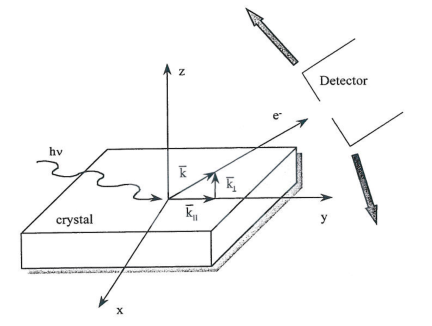
\includegraphics[scale=4]{figures/05_01.png}
	\caption{Schematics of the experimental set-up in an angle resolved UPS experiment.}
	\label{fig:arups}
	\end{center}
\end{figure}

A typical UPS spectrum of a transition metal is shown in \autoref{fig:cuups}. Here the d-band finger print can be found just below the Fermi level. It is also seen how the intensity increases towards low kinetic energy due to loss mechanisms. It is obvious that UPS cannot be used for identification of which elements that are present at the surface, since all metals (except for the rare earths) only exhibit broad and featureless structures in this region. 

\begin{figure}[h!]
	\begin{center}
	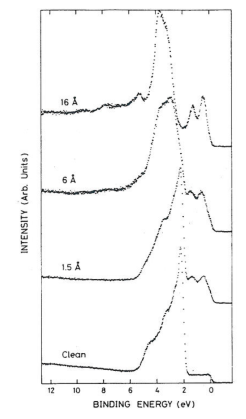
\includegraphics[scale=4]{figures/05_02.png}
	\caption{A UPS spectrum of clean Cu(100) with increasing amounts of samarium deposited. The photon energy was $h\nu=\SI{60}{\electronvolt}$. The sp-band of copper is observed just below the Fermi level, whereas the d-band is located at \SIrange{2}{4}{\electronvolt} binding energy. Taken from \cite{Andersen}.}
	\label{fig:cuups}
	\end{center}
\end{figure}

\section{The Electronic Structure}
\subsection{The Band Structure}
UPS and in particular ARUPS have been used to map out the band structure of solid materials. Here the outer electrons of the atoms react with each other forming a band structure with dispersion dependent on the momentum vector $\vec{k}$. \autoref{fig:bandstructure} shows the band structure for a simple free electron metal i.e. $E(k)=(\hbar k)^2/(2m)$. The photoemission process have to conserve both energy and momentum. Since the photon does not carry sufficient momentum to account for the momentum carried away by the photoelectron emitted the crystal must take care of the recoil. This is illustrated in the reduced zone where the electron takes up a reciprocal lattice vector and the process can be depicted as a direct transition in the reduced zone.

\begin{figure}[h!]
	\begin{center}
	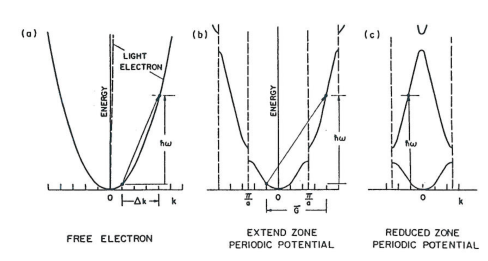
\includegraphics[scale=4]{figures/05_03.png}
	\caption{Sketch of the band structure of a free electron metal. Note the small momentum the photon carries compared to the electron. The transition can therefore only take place in the reduced zone where the lattice take up the recoil.}
	\label{fig:bandstructure}
	\end{center}
\end{figure}

By utilising the angle resolved method it is possible to map out the detailed band structure of a solid and in particular the structure at the surface region. An example is shown in \autoref{fig:cuarups} where the ARUPS spectra of Cu(111) are shown as a function of angle into the analyser using $h\nu=\SI{11.6}{\electronvolt}$.  The kinetic energy of the emitted  photoelectrons is given by

\begin{equation}
E_{kin}=h\nu-E_B-e\Phi
\end{equation}

\noindent where $E_B$ is the binding energy of the electron relative to the Fermi level, and $\Phi$ is the work function of the analyser.

\begin{equation}
E_{kin}=\frac{(\hbar k)^2}{2m}
\end{equation}

\noindent leading to 

\begin{equation}
k_\parallel=\sqrt{\frac{2mE_{kin}}{\hbar}}\sin \theta
\end{equation}

\noindent where $k_\parallel$  is the component of the momentum parallel to the surface.

\begin{figure}[h!]
	\begin{center}
	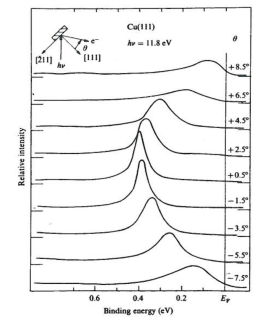
\includegraphics[scale=4]{figures/05_04.png}
	\caption{The ARUPS of Cu(111) as a function of the angle $\theta$ from the surface normal.}
	\label{fig:cuarups}
	\end{center}
\end{figure}

The momentum orthogonal to the surface $k_{\perp}$ is not conserved due to the work done by leaving the potential barrier at the surface (the work function of the crystal). By determining binding energy and $k_\parallel$ it is possible to map out the band structure around the $\Gamma$ point for Cu(111) as illustrated in \autoref{fig:cubandstructure}. The shown example is rather atypical since the shown band is a surface state lying in a bandgap. Usually there will be several bands overlapping and the gray zone indicated in \autoref{fig:cubandstructure} illustrates such  filled states in Cu(111), which in other directions will naturally cross the Fermi level since copper is known to be a metal. For a more detailed description of the band structure and how to measure it  we shall refer to \cite{Neddermeyer, Kevan}.

\begin{figure}[h!]
	\begin{center}
	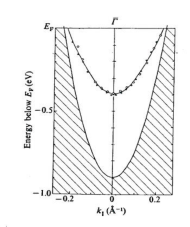
\includegraphics[scale=4]{figures/05_05.png}
	\caption{The band structure of the surface state in Cu(111) around the $\Gamma$ point. The gray zone illustrates the occupied bulk states.}
	\label{fig:cubandstructure}
	\end{center}
\end{figure}

Actually the experiment shown in \autoref{fig:cubandstructure} is a very simple example. In reality the measurement of such photoelectrons is a three step process  \cite{Berglund} where, firstly, the electron is excited from an initial band up into an empty band, secondly it have to be transported to the surface. In that process it may be diffracted as we shall see later and then  finally be detected. Thus diffraction phenomena may also have to be taken into account considering the details of such experiments.

\subsection{The Electronic Structure of Adsorbates}
When a molecule like CO (the test molecule of surface science) approaches a surface the electronic states will in general be broadened and lowered due to the interaction with the metal electrons. Thus, although the states are quite well defined in the gas phase they will now be rather broad as seen below in \autoref{fig:coups}. This figure shows the UPS spectra for gas phase CO and CO adsorbed on a number of transition metals like Ir, Ru, Pd, Pt, and Ni. The three highest occupied molecular levels of CO are easily identified in the gas phase spectrum, however, when CO chemisorbs the only feature which can be identified is due to the interaction with the valence electrons.  The contribution from the d-band is  in these late transition metals dominating the spectrum just below the Fermi level.

\begin{figure}[h!]
	\begin{center}
	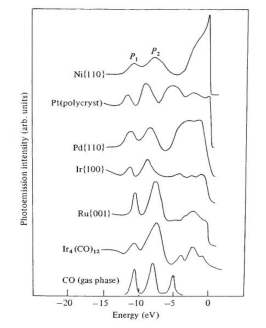
\includegraphics[scale=4]{figures/05_06.png}
	\caption{UPS of CO in the gas phase as well as CO adsorbed on a number of transition metals. Taken from Gustafson and Plummer \cite{Gustafson}.}
	\label{fig:coups}
	\end{center}
\end{figure}

Similar spectra can be observed for other adsorbates. Again it is seen that this cannot be used to identify adsorbates but solely to understand the bonding of already well defined systems. In this manner it was possible to understand the bonding geometry of for instance CO and also how molecules interact with each other as a function of coverage. Initially there was much dispute concerning the orientation of a chemisorbed molecule on a metal surface. Now it is well known that the molecule is bonded through the carbon in the "Blyholder  model"  and is standing orthogonal on the surface, at least in the low coverage regime. In the following we shall briefly demonstrate how such information can be obtained by using ARUPS and polarized light. The probability for photoelectron emission in second order time-dependent perturbation theory is given by

\begin{equation}
P_{if}=|<\Psi_{i}|{\bf H}_{int}|\Psi_f>|^2
\end{equation}

$\Psi_i$ and $\Psi_f$ are the electronic wave functions for the initial and final states and   ${\bf H}_{int}$ is the interaction Hamiltonian given by
 
\begin{equation}
{\bf H}_{int}\propto \vec{A}\cdot \vec{P}
\end{equation}
 
\noindent where $\vec{A}$ is the vector potential set up by the photon and $\vec{P}$ is the momentum operator

\begin{equation}
\vec{P}=\hbar \vec{\nabla}=\hbar \left(\frac{\partial}{\partial x}, \frac{\partial}{\partial y}, \frac{\partial}{\partial z}\right)
\end{equation}

Now lets assume that the CO molecule is adsorbed on top of a Ni atom on a Ni(100) surface which contains a mirror plane. Then the matrix element $<\Psi_i|{\bf H}_{int}|\Psi_f>$ must be invariant to such a symmetry operation, i.e. the matrix element must be even to the operation or zero. The experiment is shown schematically in \autoref{fig:arupspol}

\begin{figure}[h!]
	\begin{center}
	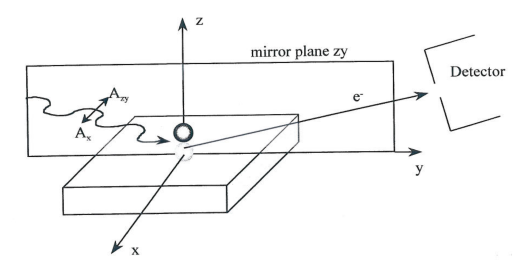
\includegraphics[scale=3.5]{figures/05_07.png}
	\caption{ An ARUPS experiment using polarised light on a surface containing a mirror plane in the $zy$-plane.}
	\label{fig:arupspol}
	\end{center}
\end{figure}

Assume the mirror plane is lying in the $zy$-plane and the detector is located in this plane as well, then the final state  $\Psi_f$ must be even with respect to the symmetry operation or zero, i.e. no signal in the detector. We then have two possibilities for the incoming light. It can either be s-polarised i.e. the vector potential only has components parallel to the surface or p-polarised where it has components orthogonal to the surface. It is then easily seen that if we consider s-polarised light the product $\vec{A}\cdot \vec{P}$ will give a product that will be odd with respect to the reflection in the $zy$-plane since $\Psi_f$ should be even if anything should be detected. Thus $\Psi_i$ must be odd in order for the matrix element to be even. Thus it is only possible to excite molecular orbitals that are odd with s-polarised light in the given configuration. This is clearly illustrated in \autoref{fig:arupsspol} where it is seen that for a certain configuration the even $4\sigma$ is vanishing in the spectrum, while the odd $1\pi$ still is observed.

\begin{figure}[h!]
	\begin{center}
	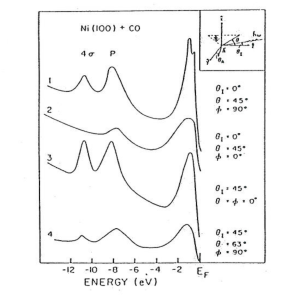
\includegraphics[scale=4.5]{figures/05_08.png}
	\caption{The result of an ARUPS experiment where the use of s-polarised light suppresses the signal from the even $4\sigma$ while the odd $1\pi$ can still be observed. For other combinations both orbitals are observed.}
	\label{fig:arupsspol}
	\end{center}
\end{figure}

The symmetry of the various orbitals of CO are reproduced in \autoref{fig:orbitals}. By playing around with the geometry like this it is possible to describe the geometry of the chemisorbed CO molecule. It has been show that the molecules tend to tilt when the coverage gets very high in order to accommodate the last CO molecules.

\begin{figure}[h!]
	\begin{center}
	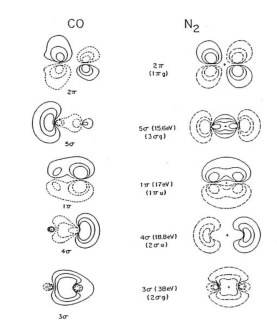
\includegraphics[scale=4.5]{figures/05_09.png}
	\caption{Sketches of the molecular orbital for CO and \ce{N2}. Notice that the $\sigma$ orbitals are even with respect to the molecular axis while the $\pi$ orbitals are odd.}
	\label{fig:orbitals}
	\end{center}
\end{figure}

The method has played a very big role in the infancy of surface science, e.g. to reveal the orientation and bonding geometry of molecules on the surface.

\section{Problems}
\begin{enumerate}
\item Calculate the momentum of a photon and convince yourself that it is much smaller than a reciprocal lattice vector.

\item Discuss to which extent UPS and XPS can be used for qualitative and quantitative investigations of surfaces.

\item What makes UPS particular usefull for studying chemisorption of molecules on surfaces? How can UPS be used to determine the binding geometry?
\end{enumerate}

%\chapter{The Auger Process}
The Auger process was first explained by  Pierre Auger in 1923 who was performing experiments with X-rays in a cloud chamber. He observed that besides the photoelectrons, which had an energy dependent on the energy of the X-rays, there were also emitted electrons with a constant energy and thus independent on which source had been used. These so-called radiationless transitions were due  to the relaxation of the electron holes in the atom created by the photoemission process. We shall from here on refer to these processes as Auger transitions. The process is illustrated in Figure 6.1.

The {\em initial state} in this case consists of an atom where a hole has been created in a deep-lying core level. As we shall see, it is not interesting how this initial state was created. This atom is now highly excited and will eventually undergo a relaxation process. In Chapter \ref{ch:xps} we saw that this relaxation can lead to emission of an X-ray photon, however, as long as the binding energy of the initial hole is well below \SI{10}{k\electronvolt} this process has a rather low probability of taking place. It is actually much more likely that a  weakly bound electron will drop down and fill the initial hole and instead of emitting a photon use the energy to excite another electron out of the atom, leading to the {\em final state}. As  shown in Figure 6.1 the final state consists of an atom with two holes either in some core levels, or in the  valence  levels or any combination thereof.

As for the photoemission process, the  kinetic energy of the emitted electron will simply be the difference between the initial state and the final state. A crude estimate will thus be given by the Koopman binding energies as

\begin{equation}\label{eq:ekinkoopman}
E_{kin}=E_{initial}-E_{final}\approx E_{B          initial}-E_{Bfinal1}-E_{Bfinal2}
\end{equation}

where $E_x$ refers to the one electron binding energy of the holes involved.

Just as in the case of XPS it is clear that the energy distribution of the emitted electron will provide a unique identification of which elements and how much of each is present in our sample. If the appropriate energy interval is chosen it will also be surface sensitive. Thus we have a method which is very  similar  to XPS. However, there are a number of differences which sometimes makes AES more useful than XPS or vice versa.

          \vspace*{14cm}

          \noindent {\bf Figure 6.1} Schematics of an  Auger  process.
          Notice that both initial and final states have two holes.\\

\section{The Excitation Source}
The major difference between AES and XPS is the manner in which we get the atoms to emit electrons. We have earlier seen (see Figure 4.7) that there will always be emitted Auger electrons as a result of the relaxation of the holes created by the photoemission process. This is however a very inconvenient way of generating the necessary initial holes for the Auger process. It is much more useful to use a high energetic electron beam typically from \SIrange{3}{10}{k\electronvolt}. As we saw under the discussion of the various energy loss mechanisms, energetic electrons will have a finite possibility of ionising the atoms in the substrate and hereby creating the necessary initial holes in a deep-lying core level (see Figure 2.10). The advantage of using an electron beam is that it can be focused and manipulated rather well and still have a high current density.
        
The electron beam is generated by use of an electron gun which is usually mounted inside the CMA as indicated in Figure 3.1. By passing current through a filament it will be heated sufficiently so that electrons can evaporate and be accelerated towards the sample. A number  of lenses ensure that the beam diameter can be controlled and deflection plates at the end of the gun ensures that the beam can be manipulated to any desired position on the surface or scan over an area (see Figure 6.2).\\

          \vspace{12cm}

          \noindent {\bf Figure 6.2} Schematics of an electron gun for
          AES.\\

As the lens system in the electron gun is an electrostatic imaging of the electron source onto the sample it is advantageous to use a \ce{LaB6} source. By mounting a \ce{LaB6} crystal on a filament a very good point source can be obtained and a spot diameter down to \SI{200}{\angstrom} can be achieved with a current of \SI{0.1}{nA}. Actually even higher resolutions can be obtained as in the  electron microscopes, but here we must remember that a sufficiently high current density is required if we want to obtain Auger spectra with a reasonable signal to noise ratio. As this demands no less than \SI{0.1}{nA} and as it is not possible to  confine electrons to spots smaller than \SI{200}{\angstrom} at such high  current  densities (unless going to much higher energies which then causes other problems) this in reality sets the limit for lateral resolution in AES.

\section{The Fine Structure in AES}
As mentioned the kinetic energy of the Auger electrons is given by the difference between the initial and final state. Thus Eq. \eqref{eq:ekinkoopman} is only very crude as we know that the atom will undergo relaxations when the initial  hole is being created. A better approximation is therefore to take the binding energy of the two final holes to be an average of the binding energy for the atom considered $Z$ and the binding energy it would have in an atom with $Z+1$. The kinetic energy could then be approximated by

\begin{equation}
E_{kin}\approx E_{Binitial}^Z-\frac{E_{Bfinal1}^{Z+1}+E_{Bfinal1}^Z+E_{Bfinal2}^{Z+1}+E_{Bfinal2}^Z}{2}
\end{equation}

where $E_x^Z$ refers to the one electron binding energy of the hole $x$ in atom $Z$. In Figure 6.3 the kinetic energy for the strongest Auger lines is given for most of the elements. It is obvious that it is nearly always possible to find an Auger line with an energy in the interval where the electrons will be surface sensitive.\\

\subsection{Nomenclature}
An Auger transition is always named XYZ describing which energy levels are participating in the transition. The X refers to the initial hole, whereas the Y and Z refers to the two holes in the final state. In order to make this more complicated than necessary the old X-ray  notation is used for these levels. Here the various levels have the following names:

\vspace{0.5cm}

             \noindent   1s   \hfill   K\\   2s,   2p$_{\frac{1}{2}}$,
          2p$_{\frac{3}{2}}$ \hfill L$_1$,  L$_2$,  L$_3$\\  3s,
          3p$_{\frac{1}{2}}$, 3p$_{\frac{3}{2}}$,  3d$_{\frac{3}{2}}$,
          3d$_{\frac{5}{2}}$   \hfill   M$_1$,   M$_2$,   M$_3$,
          M$_4$,       M$_5$\\       4s,       4p$_{\frac{1}{2}}$,
          4p$_{\frac{3}{2}}$, 4d$_{\frac{3}{2}}$,  4d$_{\frac{5}{2}}$,
          4f$_{\frac{5}{2}}$,   4f$_{\frac{7}{2}}$   \hfill   N$_1$,
          N$_2$,  N$_3$,  N$_4$,  N$_5$,  N$_6$,   N$_7$\\


         \newpage
          \vspace*{14cm}

          \noindent {\bf Figure 6.3}  Energies  of  the  strongest
          Auger transitions.


\subsection{Mulitiplet Splitting in AES}
If we consider a transition starting with  a hole in the 1s shell which results in two holes in the 2s or 2p shell then the name of the transition would be KLL which is the dominant type of lines for the lighter elements. This type of transition can naturally be divided up into different combinations like: KL$_1$L$_1$, KL$_1$L$_2$, KL$_1$L$_3$, KL$_2$L$_3$, KL$_2$L$_2$, KL$_3$L$_3$ leading to six lines.

In Figure 6.4 this type of transition is shown for magnesium and it is easily seen that the spectrum cannot be explained by only four lines. The reason that we only got six lines is that we used a notation  only appropriate in jj-coupling. We saw earlier that when more than one localised hole is present it is more appropriate to use intermediate coupling starting either from jj-coupling or LS-coupling.\\

        \noindent {\bf Figure 6.4} A KLL Auger\\ spectrum of Magnesium\\

             \vspace*{9cm}

Thus in the intermediate coupling scheme the above transitions would lead to the following final states:

             \vspace{0.5cm}

          \noindent     KL$_1$L$_1$      \hfill      $^1S_0$\\
          KL$_1$L$_2$,           KL$_1$L$_3$            \hfill
          $^1P_1$,$^3P_0$,$^3P_1$,$^3P_2$\\
          KL$_2$L$_3$, KL$_2$L$_2$,  KL$_3$L$_3$   \hfill
          $^1S_0$,$^3P_0$,$^3P_1$,$^3P_2$,$^1D_2$\\

          \vspace{0.5cm}

Thus the simplest transition we can think of consists of a substantial number of lines. If the initial state is not an s-electron there will also be a splitting of the initial state due to a spin orbit splitting doubling the number of Auger lines. An example of this type of transition is shown in Figure 6.5 where the M$_{45}$N$_{67}$N$_{67}$ for ytterbium and gold are shown. The spin-orbit splitting of the N$_{45}$ level is very large in both cases leading to two well-separated multiples. A theoretical description of the line shape (using the intermediate coupling  scheme) is possible for the gold, but not for the ytterbium where other types of Auger transitions obscure the comparison. Due to an M$_{4}$M$_{5}$N$_{67}$ there will be a transition starting with a hole both in the M$_{5}$ and the N$_{67}$ level leading to a multiplet structure right on top of the M$_{5}$N$_{67}$N$_{67}$ lines. The spectra shown in Figure 6.5 was actually induced by the continuous bremsstrahlung emitted from an aluminium anode.\\

          \vspace*{15cm}
          \noindent {\bf Figure 6.5} The experimental Auger spectra of
          Yb and Au and the theoretical fits.\\


So far we have not discussed the transition probability for the Auger transition. As the relaxation process is due to the Coulomb interaction between the involved electrons, the interaction Hamiltonian will be described by a Coulomb interaction and the transition probability will be given again by Fermi's golden rule. In the frozen core approximation and one-electron picture this results in \cite{wentzel}:

\begin{equation}
P_{Auger}=\frac{4\pi^2}{h}\vert \left< \Phi_{Initial}\vert \frac{e^2}{r_{12}}\vert \Phi_{Final}\right>\vert ^2
\end{equation}

where initial and final states refers to the two vacancies in the initial and final state. This expression has been used to calculate the probability for going from each possible initial state to any available final state as shown in Figure 6.5. In general the multiplet splitting of Auger transitions is quite complex leading to rather broad features as we have already seen. The lifetime broadening will contribute significantly as there are three holes involved in the process now. Furthermore, just as was  the case for the photoemission process, the Auger process will be followed by various shake-up and shake-off processes leading to satellite structures. They are therefore not as useful for chemical identification and investigations of electron structures as the XPS lines. But if we disregard the details of the structure and simply use the Auger lines as a finger print of the various elements they can be very useful.

\section{AES for Qualitative Analysis}
When creating a deep lying hole there are two competing possibilities for relaxation of the excited atom. One is the emission of a photon with the probability $\omega_{X}$, which was very useful for generation of X-rays for XPS, and the other is a decay through emission of an Auger electron with the probability $\omega_{Auger}$. The two channels are competing, but in general $\omega_{Auger}$ will be much larger than $\omega_{X}$ for initial holes with binding energy less than \SI{10}{k\electronvolt}. For example Figure 5.6 shows the probability of the two types of  relaxation plotted for a hole in the 1s shell as a function of the atomic number. The binding energy of the 1s level in element $Z=33$ (As) is \SI{11.8}{k\eelectronvolt}. Thus for electron beams with energy less than \SI{10}{k\electronvolt} the Auger process will prevail.\\

          \vspace{1cm}

          \noindent {\bf Figure 6.6} $\omega_{X}$ and  $\omega_{A}$\\  as  a
          function of Z\\ for the 1s shell.\\

          \vspace{4cm}

The emission of the X-rays actually has a  very useful aspect since they also carry information on which elements are present in the sample. This method is known by the name EDX and is mainly performed in combination with electron microscopy. It is complementary to the methods discussed here as it is not surface sensitive (usually probing $\sim \SI{1}{\micro m}$) on the atomic scale. Besides it is not a very useful method for detection of the light elements ($Z<11$) as most of the relaxation in this low binding energy regime takes place through Auger transitions.

An Auger spectrum of silver excited by the use of \SI{2}{k\electronvolt} electrons is shown in Figure 6.7. The $N(E)$ spectrum is completely dominated by the elastically scattered electrons and primary electrons which have undergone energy losses in the solid.\\

          \vspace{9.5cm}

          \noindent {\bf Figure 6.7} The raw N(E)  spectra  of  Silver
          excited by 2 keV electrons.\\

Weak structures can be observed just below the elastic peak (energy loss features of silver) and around \SI{350}{\electronvolt}. This region has also been shown as $N(E)\times 10$ and it is now easily seen that there is a structure here. By consulting Figure 6.3 these lines can be identified as the silver M$_{45}$N$_{45}$N$_{45}$ transition. The lines are lying on top of the high continuous background of secondary electrons which basically carries no information and it is therefore convenient to differentiate the spectrum as shown in the top panel. The nearly constant background is then eliminated and the structure of the line is easily recognised. The intensity of the lines, assuming a Gaussian line shape, can then be approximated by the peak to peak height. Just as for XPS all the Auger spectra of the elements have been collected in a handbook \cite{handbook} and Figures 6.8 and 6.9 show a few examples of such standard Auger spectra.
          \newpage

          \vspace*{10.5cm}

                  \noindent {\bf Figure 6.8} The standard  Auger  spectrum  of
          Aluminium.\\


             Figure 6.8 shows the Auger spectrum of a  relative  clean
          Aluminium surface. Apart  from  several  low  level
          contamination features of Ar, C, and O, two main features from
          Aluminium are observed. The low lying line at 68 eV  is  due
          to an L$_{23}$VV transition. The VV refers to the  fact  that
          the two final states are located in the valence band and the
          shape of the Auger line in this case will actually be a self
          convolution of the valence band. The high energetic line  at
          1396 eV is due to a KL$_{23}$L$_{23}$  transition  which  is
          much weaker. The features below 1390 eV can be accounted for
          by energy losses to plasmons. If this surface is oxidised to
          Al$_{2}$O$_{3}$ the spectrum undergoes rather strong changes
          as shown in Figure 6.9. Both transition shifts downwards  in
          energy by 17-18 eV and  the  energy  loss  features  change
          dramatically. This  is  a  result  of  chemical  shifts  and
          changes in the relaxation mechanisms. The Aluminium  has  by
          oxidation been changed from a  very  good  conductor  to  an
          isolator. Thus the valence electrons have been shifted down in
          energy and there are no delocalised electrons around to
          effectively screen the excited final state. Therefore, the
          characteristic plasmon energy losses are no longer observed.
          In this case it is possible to identify the chemical
          state of the Aluminium, especially when the presence of
          oxygen at 510 eV is taken into account. \newpage 

           \vspace*{10cm}

          \noindent {\bf Figure 6.9} The standard  Auger  spectrum  of
          Al$_{2}$O$_{3}$.\\


             Similar chemical identification can be done for carbon as
          seen in Figure 6.10. Here the carbon Auger feature is depicted
          for a number  of  carbon  containing  compounds.  It  is  in
          general possible to differentiate between carbon in covalent
          bonding and ionic bonding. The carbides display a  spectrum
          characteristic of a filled shell structure  like  Neon.  The
          same features are observed  for  Nitrogen  in  nitrides  and
          naturally for Oxygen and Fluorine. Figure 6.11 shows  an
          AES study of the decomposition of methylamine on Nickel. At
          very low temperatures the methylamine is chemisorbed
          associatively on the surface and the spectrum reflects to a
          high degree the line shape expected from molecules. As the
          surface is heated the molecule will decompose and finally
          all the hydrogen will desorb and the Nitrogen and Carbon
          will react with the surface forming carbides and nitrides
          which can easily be identified by their characteristic line
          shapes \cite{chorkendorff3}.

          Thus chemical identification  can  sometimes  be  undertaken
          with AES, but  certainly  not  as  efficiently  as  with  XPS.
          Besides there are other problems with AES  which  should  be
          mentioned when discussing chemical identification.  Since  a
          high energetic electron beam is used with  a  relatively  high
          current density, there is always a potential danger that  the
          excitation source itself introduces chemistry. This is not  a
          severe problem for metals and alloys, but it is serious for
          chemical compounds like polymers or the methylamine shown
          above.

             \newpage \noindent {\bf Figure 6.10} The auger line
          shape\\ of the KLL transition in various\\ chemical
          surroundings. 

                                 \vspace{9cm}

             \noindent  {\bf  Figure 6.11}  The  Auger  spectrum \\  of
          methylamine adsorbed on Ni(111)\\ during decomposition.

                                           \newpage



           If the AES spectrum of the chemisorbed  methylamine
          shown in the bottom of Figure 6.10 was  repeated  after  the
          surface has been exposed to the electron beam for 5 min  the
          spectrum would look exactly as if it had reacted all the way
          to Nickel-nitride and -carbide. Thus great care  has  to  be
          taken when AES is used on compounds.


             \section{AES for Quantitative Analysis}

             Carrying out quantitative analysis with AES is very
          similar to XPS, although there are few complicating factors.
          The probability for getting an Auger electron XYZ out from a
          thin layer of element x in the depth z will be given by
          \begin{equation} dI^{XYZ}_{x}(z) = N_{x}\sigma_{X}(z)
          \omega_{XYZ} e^{-\frac{z}{\lambda_{XYZ}}} i(z) T(E_{XYZ}) dz
          \end{equation} where N$_{x}$ is the number of
          atoms$\times$cm$^{-3}$, $\sigma_{X}(z)$ is the cross
          section for generating the initial hole X in the depth z,
          $\omega_{XYZ}$ is the probability that the initial hole will
          decay as an Auger process, ${\lambda_{XYZ}}$ is the
          inelastic mean free path of the Auger electron, T(E$_{XYZ}$)
          is the probability that the electron will be detected by the
          analyser, i(z) is the flux of primary electron in the depth
          z. The electron flux of primary electrons vary with the
          depth because these electrons will undergo energy losses and
          because they will scatter elastically in the solid. 

             If we  consider  a  pure  element  and  assume  that  the
          dependency on depth is weak all these various factors can be
          put  together  in  one  constant   namely
            \begin{equation}
          I^{\infty  XYZ}_{x}   =   N_{x}\sigma_{X}   \omega_{XYZ}   i_{0}
          T(E_{XYZ})\lambda_{XYZ} \end{equation} which is the  signal
          we will obtain from the clean sample.
             Equation 6.3 would then read
            \begin{equation}
          dI_{x}^{XYZ}(z)  =   \frac{I^{\infty   XYZ}_{x}}{\lambda_{XYZ}}
          e^{-\frac{z}{\lambda_{XYZ}}}dz
          \end{equation}
             By integration from zero depth to infinity we get
               \begin{equation}
          I^{\infty   XYZ}_{x}   =   \int   dI_{x}^{XYZ}(z)    =
          \int_{0}^{\infty}\frac{I^{\infty     XYZ}_{x}}{\lambda_{XYZ}}
          e^{-\frac{z}{\lambda_{XYZ}}}dz \end{equation}
          By measuring  the  signal  from  the  pure  elements  it  is
          possible to establish a set of sensitivity factors just as it
          was done for the XPS lines.
               \begin{equation}
          I^{XYZ}_{x} = S_{x}^{XYZ} N_{x}
          \end{equation}
             whereby the composition of a sample can be estimated as
                  \begin{equation}
           C_{x}                                                      =
          \frac{\frac{I^{XYZ}_{x}}{S_{x}^{XYZ}}}{\sum_{i}^{N}\frac{I^{XYZ}_{i}}{S_{i}^{XYZ}}}*100\%
            \end{equation}
          where the sum i goes over all N elements present in the sample.

             The  relative  sensitivity  factors  for  most   of   the
          strongest Auger lines are shown in Figure 6.12 for a primary
          electron beam of 3 keV and in Figure 6.13 for a primary beam
          of 10 keV. Both Figures are taken from \cite{handbook}.

          \vspace{12cm}

             \noindent {\bf Figure 6.12} The sensitivity  factors  for
          Auger transitions excited by 3 keV electrons.\\

          Several  approximations  were   necessary   to   achieve   this
          simple expression and the compositions determined  in  this
          manner will therefore also have a considerable  uncertainty.
          Thus  for  investigations  where  accurate  determination  of
          the surface composition is mandatory  XPS  should  be  used.
          However, the  AES  method  is  very  useful  especially  for
          determining relative compositions between different areas of
          the samples or  depth analysis.
          \newpage

                  \vspace*{12cm}

             \noindent {\bf Figure 6.13} The sensitivity  factors  for
          Auger transitions excited by 10 keV electrons.

          \subsection{Example}
          In this example we shall demonstrate how the attenuation  of
          the Auger signals can be used to study growth  mechanisms  on
          surfaces and how it can be used to determine  the  inelastic
          mean free path.  Figure 6.14 shows the  natural  logarithm  of
          the Auger signal for two Germanium  lines  relative  to  the
          pure Germanium   as  a  function  of  Silicon  coverage
          deposited on top of the  Germanium.  It  is  seen  that  the
          Germanium signal is damped exponentially. If we assume  that
          the analyser was positioned normal to  the  surface  we  can
          estimate $\lambda$ for the two different  kinetics  energies
          if the coverage of the Silicon is known  and  if  we  assume
          that it is deposited layer by layer.
          The Germanium intensity will be given by
          \begin{equation}
          I^{XYZ}_{Ge}(d_{Si})=I^{\infty XYZ}_{Ge}e^{-\frac{d_{Si}}{\lambda_{Si}}}
          \end{equation}
          where $d_{Si}$  is  the  thickness  of  the  overlayer.  The
          Germanium signal will be damped through the Silicon and it is
          therefore $\lambda_{Si}$ which is determined in this manner.

          \noindent {\bf Figure 6.14} Attenuation of the\\ Ge LMM  (1147
          eV) and Ge MVV\\ (52eV)  Auger  lines  as  a\\  function  of  Si
          Coverage.\\

                      \vspace{9cm}

          By plotting ln($\frac{I^{XYZ}_{Ge}(d_{Si})}{I^{\infty    XYZ}_{Ge}}$)
          vs. d$_{Si}$,  $\lambda_{Si}$  can  be  found  for  the  two
          energies.

             Similarly the signal of the  Silicon  Auger lines  can  be
          followed and the intensity of the Silicon Auger lines  would
          have the following form as a function of  thickness
          \begin{equation}
          I^{XYZ}_{Si}(d_{Si})=\int_{0}^{d_{Si}}\frac{I^{\infty
          XYZ}_{Si}}{\lambda_{Si}}e^{-\frac{z}{\lambda_{Si}}}dz=I^{\infty
          XYZ}_{Si}(1-e^{-\frac{d_{Si}}{\lambda_{Si}}})
          \end{equation}
          The above results can easily be made more surface  sensitive
          by changing the detection angle to be $\theta$  degrees  off
          normal. $\lambda$ would then in the above formulas change to
          $\lambda*cos(\theta)$ as we saw in eqn 4.26

          \subsection{Growth Mechanisms}

          The availability to grow new structures on a substrate is today
          a very important field in material  science.  In  the  above
          example we assumed that the growth  of  the  Silicon  was  a
          layer by layer mechanism. Thus one layer of Si is  completed
          before the next layer is started and it is possible to  grow
          perfect macroscopic crystal structures in this manner. If  we
          look carefully at the Germanium signal as a  function  of  the
          Silicon coverage, we  shall  see  that  the  signal  actually
          consists  of  a  number  of  straight   lines   which   form
          an exponential decay. The ratio of the Germanium signal for a
          coverage of $\theta_{Si}$ less than one  monolayer  will  be
          given                  by                   \begin{equation}
          \frac{I_{Ge}(\theta_{Si})}{I_{Ge}^{\infty}}                =
          (1-\theta_{Si})+\theta_{Si}e^{-\frac{l_{Si}}{\lambda_{Si}}}
          \hspace{2cm} 0\leq \theta_{Si} \leq 1  \end{equation}  where
          l$_{Si}$ is the thickness of one monolayer of Silicon.

             The above equation  can  easily  be  generalised  to  the
          transition from the n$^{th}$ layer to the (n+1)$^{th}$ layer

          \begin{equation}
          \frac{I_{Ge}(\theta_{Si})}{I_{Ge}^{\infty}}                =
          (1-\theta_{Si})e^{-\frac{nl_{Si}}{\lambda_{Si}}}+\theta_{Si}e^{-\frac{(n+1)l_{Si}}{\lambda_{Si}}}
          \hspace{2cm} 0\leq \theta_{Si} \leq 1 \end{equation} where  $\theta_{Si}$
          is the amount of the n$^{th}$ layer covered with Silicon.

          The result of such an attenuation of the Germanium signal is
          shown in Figure 6.15.\\

          \vspace{9cm}

          \noindent {\bf Figure 6.15} The attenuation of the substrate
          signal as a  function  of  coverage.  The  different  curves
          represents different growth mechanisms.\\


          Unfortunately the growth mechanisms are in  general  not  as
          simple as we just have seen. They are  dictated  by  surface
          diffusion,  deposition  rates,  substrate  temperature,   and
          surface and interface energies of the elements involved.  It
          is beyond the scope of this review to go further into the
          various mechanisms, but we shall mention that there are
          other categories of growth.

            \begin{itemize}

          \item The layer by layer growth is called  a  {\bf  Frank-van  der
          Merwe growth}.

          \item Another possibility is that the first  layer  is  completed
          before the second layer is started, but then  the  layer  by
          layer growth stops and islands are formed. This is called  a
          {\bf Stranski-Krastanov growth} mode.

          \item Finally there is the possibility  that  islands  are  formed
          right from the beginning and that is referred to as  a  {\bf
          Volmer-Weber} growth mode.

                \end{itemize}
          It is only in the first case it is possible to describe  the
          process easily. In the other modes the unknown  distribution
          of islands and their sizes makes an analysis  very  difficult.
          The effects of the various  mechanisms  are  illustrated  in
          Figure 6.15.

          Recent experiments by using  Scanning  Tunnelling  Microscopy,
          where it is possible to  investigate  the  individual  atoms
          deposited on the surface, have shown that alloying   also
          complicates the above picture.

          \section{Scanning Auger Microscopy SAM}


          The maybe biggest advantage of AES is the availability
          to focus the primary electron beam to a  small  spot  as  we
          discussed in section  6.1.  Thus  very  small  areas  can  be
          analysed. If this is combined with the possibility  to  scan
          the electron beam over the surface it is possible to  obtain
          a lateral resolution of the surface  composition.

          Figure 6.16 shows an Auger spectrum of a Copper  grid  placed
          on top of a Silver foil. There are 25$\mu$m  between  each
          mask of the grid and the Auger spectrum was obtained  while
          the electron  beam  was  scanned  over  an  area  of  65$\times$100
          $\mu$m$^{2}$ with TV scan rate.\\




          If the  amount  of  secondary  electrons  emitted  from  the
          surface is measured as a function of the beam  position  it
          is possible to construct an image of the  surface.  This  is
          usually referred to as a secondary electron micrograph which
          can give a topologic information of the surface .  The  top
          panel of Figure 6.17 shows such a SEM picture of the  Copper
          grid.



          If now the analyser is set to measure the  intensity  in  a
          narrow window around for example the silver line at 355 eV it
          is possible to measure the amount of Silver in  the  surface
          as a function of the electron beam position. This is exactly
          what has been done in the rest of the panels in Figure 6.17
          for a number of the elements seen  in  Figure 6.16.  It  is
          easily seen that the grid consists of Copper and that  it  is
          placed on top of an Silver foil. Furthermore it is observed that
          the contamination by sulphur is  primarily  located  on  the
          Silver, whereas the  Chlorine  is  mainly  adsorbed  on  the
          Copper grid.  The  resolution  in  this  picture  is  around
          1$\mu$m.

  \newpage
          \vspace*{12cm}

         \noindent {\bf Figure 6.16} The Auger spectrum of  a  Copper
         grid mounted on a Silver foil and averaged over  an  area  of
         65$\times$100 $\mu$m.\\

             The methods can be refined  by  measuring  not  only  the
          intensity of the Auger line, but also the intensity  of  the
          background before and after the peak.  In  this  manner  the
          (Signal-Background)/Background can be used for  the  imaging
          and hereby topologic effects will be reduced.

          SAM is a rather time  consuming  process  dependent  on  the
          resolution required and the size of the  area  investigated.
          In general at  least  10  ms  is  required  for  each  point
          measured  (dependent  of  the  primary  current   and   thus
          dependent of the resolution of the electron beam) and  if  a
          high resolution is needed 512$\times$512  point  may  be  required.
          Such a picture will then take 2500 seconds  and  three  time  as
          long  if the background should be eliminated.

          The method is very useful in many  contexts,  especially  in
          applied material science.\\
          \newpage

          \vspace*{18cm}

          \noindent {\bf Figure 6.17} a)The SAM picture of a Copper grid
          mounted on a Silver foil. The first picture is  a  Secondary
          Electron Micrograph picture showing the  grid.  Then  follows
          the SAM pictures of b) Cu, c) Ag, d) S, and e) Cl. 

               \newpage

          \section{Problems}
             \begin{enumerate}


             \item Estimate from Figure 6.14 the mean free path for
          electrons 52 eV and 1147 eV through Si, respectively.

             How does these data fit into the universal curve shown in
          figure 2.6?


             Discuss how the signals in Figure 6.14 would behave
          if we did not have  Van der Merwe growth.

             \item Determine how the signal of Si  will  behave  as  a
          function of dosage when it  is  evaporated  onto  Ge  as  in
          Figure 6.14.

             Hint: Plot $ln(1-\frac{I(d)}{I_{0}\lambda})$ vs d where d
          is the thickness of the overlayer.





             \item In order to get a reasonable signal to noise ratio
          it is necessary to have an electron beam current of at least
          2 nA when doing AES or SAM. Estimate the fluency when the
          beam (10 KeV) is focused to a diameter of 1 $\mu$m or 200 �
          respectively. 200 � is the ultimate resolution that can be
          achieved with SAM in dedicated equipment. In the following
          we shall assume that the cross section for dissociation of
          an adsorbed molecule by the above electrons is $\approx$
          $1*10^{-20} m^{-2}$ and that we are measuring on a monolayer
          of molecules (5*10$^{14} cm^{-2}$). How long time can we
          allow ourselves to be measuring at the same point if we only
          allow for 10 \% of the molecules to dissociate. 


             \item Figure 6.18 shows an AES spectrum of fractured
          interface between inconel 600 plate on which a ceramic
          containing Al$_{2}$O$_{3}$ and MgO was adhered. Estimate
          the surface composition of the fracture if it is assumed
          that the surface region is homogeneous. The relevant surface
          sensitivity factors are given for peak to peak measurements.
          (Inconel 600 is an alloy containing roughly 76 \% Ni, 17  \%
          Cr and 7 \% Fe).

                       \newpage

                       \vspace*{13cm}

                       \noindent {\bf Figure 6.18}





\end{enumerate}



%\chapter{Depth Profiling with XPS and AES}
In the previous chapters we have discussed the XPS and AES methods for surface analysis. Both methods are very useful for determination of the qualitative composition, although XPS clearly is the most advantageous for identifications of chemical composition and when an accurate quantitative determination is called for. On the other hand, AES is advantageous if information of the lateral composition is necessary. Both methods can also be used for a determination deeper into the material. We have already seen that some depth information can be obtained by tilting the sample relative to the analyser. This, however, only gives a depth resolution of a few atomic layers. Therefore, the methods must be combined with other methods so that the interesting layer can be exposed to the surface sensitive analysis. This can be done mechanically by a broad variety of polishing procedures or by sputtering.

\section{Instrumentation}
The first class of methods is the mechanical type where the interesting part of the sample can be exposed simply by making a cut orthogonal to the surface or by ball cratering. In the first case the deep lying layers can then be analysed by use of SAM (see Fig. \ref{fig:samorthcut}). It is immediately seen that the resolution of this analysis will be limited by the resolution of the SAM available. This may not be trivial as it is not always easy to prepare a sample with a perfect cut orthogonal to the surface, especially not in the cases where the region is very inhomogeneous. The ball cratering method, as shown in \autoref{fig:ballcrater}, is very similar except that a crater is polished in the surface. Different layers will then be exposed and can again be analysed by use of SAM with sufficient resolution.

In both cases the depth resolution is given by SAM (\SI{200}{\angstrom} and upwards), although it can be improved considerably in the ball cratering method due to the fact that we here have a cut under an angle. These methods are seldom used because in general it is much more convenient to use EDX on such samples.

\begin{figure}[h!]
	\begin{center}
	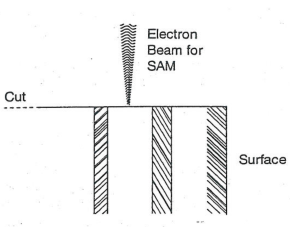
\includegraphics[scale=3]{figures/07_01.png}
	\caption{Sketch of SAM analysis of an orthogonal cut.}
	\label{fig:samorthcut}
	\end{center}
\end{figure}

\begin{figure}[h!]
	\begin{center}
	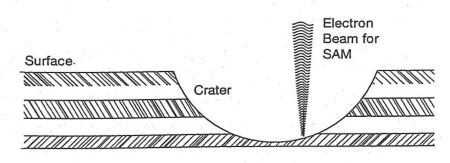
\includegraphics[scale=3]{figures/07_02.png}
	\caption{Sketch of the ball cratering method.}
	\label{fig:ballcrater}
	\end{center}
\end{figure}

However, in the range \SIrange{0}{1000}{\angstrom} there is another method by which the surface can easily be exposed and analysed by use of both AES or XPS, namely by sputtering with rare gas atoms, preferentially argon. By ionising Argon at a high potential the ions created can be manipulated just like the electrons and be focused into a spot on the surface and scanned if necessary. The formation of the beam is very similar to the way we measured the pressure in the chamber as shown in \autoref{fig:ion_gauge}. Instead of collecting the ions on the collector they are extracted from the cage formed by the grid and accelerated towards the sample which is usually kept grounded. In this manner ion beams with energies of \SIrange{1}{5}{k\electronvolt} and with currents of \SIrange{0}{10}{\micro A} can be formed. The argon is supplied by leaking in argon in the chamber to the required pressure of roughly \SI{1e-5}{mbar}. This is a high pressure in the context of UHV and might also cause problems for some types of pumps, like for instance the ion pumps, but as the gas is inert it does not influence the surface analysis if the argon is sufficiently clean. The pressure in the chamber can be reduced about three orders of magnitude if a differentially pumped ion gun is used instead. In this case a high pressure is still needed in the ionising region but the beam is then passing through a small hole into the main chamber. By pumping the ion-gun and the main chamber by separate pumps (differentially pumped) the pressure in the main chamber may be kept in the \SI{e-8}{mbar} region. The spot size diameter is, as for the electron beam, determined by the current density and will typically be on the order of \SI{100}{\micro m} in standard equipment. The beam can be scanned to give a homogeneous exposure over a rather large area ($\SI{10}{mm}\times\SI{10}{mm}$) of the surface so depth analysis with XPS can be carried out. For other applications, like for instance Secondary Ion Mass Spectroscopy (SIMS), the beam can be focused down to much smaller spots sizes.

\section{Ion Sputtering}
Several types of rare gases can be used for sputter profiling, but usually argon is the preferred gas as it is cheap to purify and has a high sputter yield. When a high energetic ion is hitting the surface the ion will be neutralised and transfer energy to the surface atoms through a number of essentially binary collisions. Some of the surface atoms will obtain sufficient energy and momentum to be able to escape the surface (see Fig. \ref{fig:sputtering}). The atoms which in this manner are scattered off the surface will mostly leave as neutral species and only a small fraction will survive as ions. Since the ions are essentially coming from the top most layer and since they are easily detected by a mass spectrometer this is a method very useful for determining the depth composition into the surface as the atoms are sputtered away. This method is called SIMS as mentioned above and can be carried out in small spots. The method is extremely sensitive (ppm level) but is rather difficult to quantify since the survival of the ions depend exponentially on the work function of the surface. For further details on this method we shall refer the reader to \cite{briggs2}. A method has been developed which overcomes this problem by detecting all the atoms coming off the surface. This is a much more reliable way to determine the surface depth composition. However, since this method relies on resonance ionisation by two lasers it is not economically viable.

Therefore, it is much more convenient to simply use either XPS, or preferentially AES, to measure what is left on the surface after a certain number of atoms have been sputtered away by bombarding the surface with energetic \ce{Ar+} ions. The measurements can be made simultaneously with sputtering or by alternating between sputtering and measuring. The AES method is the preferred method because it is in general much faster than the XPS method.

\begin{figure}[h!]
 	\begin{center}
 	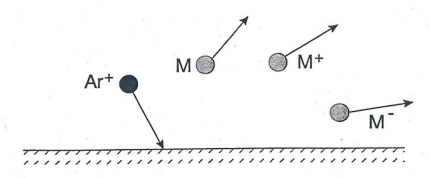
\includegraphics[scale=3]{figures/07_03.png}
 	\caption{Sketch of the sputtering process.}
 	\label{fig:sputtering}
 	\end{center}
 \end{figure} 

If we define a sputter yield $Y$ as the number of atoms removed from the surface per incoming ion it is possible, under ideal conditions, to convert time sputtered to a depth.

The flux of ions $F$ can be written as
 
\begin{equation}
F=\frac{I}{eA}
\end{equation}

\noindent where $I$ is the ion current and $A$ is the area exposed to the ion beam. In a pure element the number of atoms removed per second per area will be given by

\begin{equation}
g_i=FY_i
\end{equation}

$g_i$ can be converted to a depth by

\begin{equation}
\frac{dz_i}{dt}=\dot{z}_i=\frac{g_i}{N_i(z)}=\frac{FY_i(z)M_i}{\rho_i(z)N_A}=\frac{IY_i(z)M_i}{eA\rho_i(z)N_A}
\end{equation}

\noindent where $N_i$ is the density of atoms in the surface, $M_i$ is the mol weight, $N_A$ is Avogadro's number, and $\rho_i$ is the density of this particular element $i$. If we assume that $F$, $Y_i$, and $\rho_i$ are constants with respect to time this differential equation can easily be solved and the result is

\begin{equation}\label{eq:sputterdepth}
z(t)=\int_0^t\dot{z}dt=\frac{FYM}{\rho N_A}t=\frac{IYM}{eA\rho N_A}t
\end{equation}

This was a rather trivial example since it only applies for pure elements. Let us instead look at a two component mixture of $A$ and $B$ where we want to determine the depth compositions ($C_A(z)$ and $C_A(z)$). If we have two components, there will most likely be a difference in sputter yield for the two components leading to

\begin{equation}
z(t)=\int_0^t[C_A(t)\dot{z}_A+C_B(t)\dot{z}_B]dt 
\end{equation}

Since $C_A(z)$ and $C_A(z)$ can be estimated by the surface analysis as a function of time and since $\dot{z}$ can be estimated if the sputtering yield is known, it is possible to construct a plot showing the concentration profile of $A$ and $B$ into the material as a function of depth. Unfortunately it is generally not so simple since the sputtering yields for different compositions and compounds are not well known.

\subsection{The Sputter Yield}
The essential parameter for doing sputter profiling is the yield $Y$; the number of particles that is removed from the surface per incoming ion. The yield from a pure amorphous target can formally be written as

\begin{equation}
Y=\Delta F(E_0)
\end{equation}

\noindent where $\Delta$ is a factor containing all the material properties such as the surface binding energy of the atoms sputtered and $F(E_0)$ is the energy deposited at the surface depending upon the type of ions, the energy $E_0$, the incidence angle of the ions, the target atoms, and the density of the atoms in the target.

The parameter $\Delta$ can be derived describing the number of target atoms that obtains sufficient energy and momentum in the correct direction so that they can overcome the barrier and escape the surface. The result is

\begin{equation}
\Delta\approx\frac{0.042}{NU_0}
\end{equation}

in units of [\si{\angstrom /\electronvolt}] where $N$ [\si{\angstrom ^{-3}}] is the density of atoms in the target and $U_0$ [\si{\electronvolt}] is the surface binding energy of the target atoms. For details of the derivation of this expression we shall refer the reader to \cite{sigmund}. In \autoref{fig:xesputteryield} the sputter yield for \SI{400}{\electronvolt} \ce{Xe+} ions is plotted for most of the elements. It is clearly seen that there is a rather strong variation. More relevant data can be found in \cite{behrisch} where sputter yields for various ions, energies, and elements have been collected. All this works relatively well for the pure elements, but as soon as we turn to inhomogeneous samples consisting of alloys or compounds these sputter yields are in general not valid any longer since the surface binding energy changes for instance. Thus there is a general problem in converting the sputter time into a depth for more complex samples.

\begin{figure}[h!]
	\begin{center}
	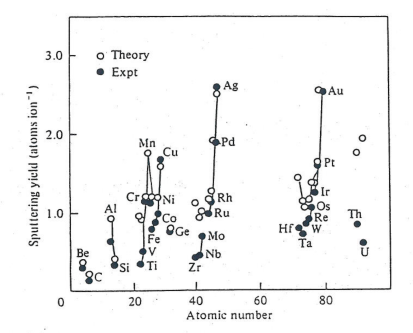
\includegraphics[scale=4]{figures/07_04.png}
	\caption{The sputter yield for \SI{500}{\electronvolt} Xe ions.}
	\label{fig:xesputteryield}
	\end{center}
\end{figure}

\section{Factors Limiting Depth Resolution and Accuracy of Profiles}
It is straight forward to perform a sputter profile and plot the concentration of the various components as a function of sputter time or even better as a function of ion dosage. The problem arises when we want to interpret these data in terms of depth and depth resolution.

\subsection{The Effect of Attenuation}
First of all, the AES-signals are not coming from a single layer but are exponentially damped signals from several layers. This means that we can never expect to obtain extremely sharp features, although the sample studied consists of such. Consider for example a thin layer of gold ($d_{\ce{Au}}=\SI{25}{\angstrom}$) deposited on top of a germanium surface and then covered by another layer of germanium $d_{\ce{Ge}}=\SI{30}{\angstrom}$. It is assumed that the deposition is ideal, i.e. it is a layer by layer growth mode (see Fig. \ref{fig:geattenuation}). We can easily adapt Equations \eqref{eq:gesignal} and \eqref{sisignal} to describe the intensities from the constructed sandwich. The signal from the gold will be given by

\begin{equation}
I_{\ce{Au}}=I^{\infty}_{\ce{Au}}\left(1-e^{-\dfrac{d_{\ce{Au}}}{\lambda_{\ce{Au} in \ce{Au}}}}\right)e^{-\dfrac{d_{\ce{Ge}}}{\lambda_{\ce{Au} in \ce{Ge}}}} 
\end{equation}

\noindent which is the gold signal from a gold layer of thickness $d_{\ce{Au}}$ damped through a germanium layer of thickness $d_{\ce{Ge}}$. The term $\lambda_{x in y}$ refers to the mean free path of an Auger electron from element $x$ moving through element $y$. Similarly, the signal from the germanium can be written as

\begin{equation}
I_{\ce{Ge}}=I^{\infty}_{\ce{Ge}}\left(1-e^{-\dfrac{d_{\ce{Ge}}}{\lambda_{\ce{Ge} in \ce{Ge}}}}\right)+ I^{\infty}_{\ce{Ge}}e^{-\dfrac{d_{\ce{Ge}}}{\lambda_{\ce{Ge} in \ce{Ge}}}-\dfrac{d_{\ce{Au}}}{\lambda_{\ce{Ge} in \ce{Au}}}}
\end{equation}

\noindent where the first term is due to the germanium overlayer and the second term is due to the germanium substrate which is damped both through the gold layer and the germanium overlayer.

This sandwich can now be analysed by sputter profiling. If it is assumed that the sputter profiling, just as the deposition, is ideal i.e. the removal takes place layer by layer it is easy to set up the equations describing the signals as a function of time. The sputter rate can be evaluated for each of the elements (Eq. \eqref{eq:sputterdepth}) and the thickness of the various layers can then be estimated as a function of time as $d-\dot{z}t$. If it takes $t_{\ce{Ge}}$ seconds to sputter through the germanium overlayer and $t_{\ce{Au}}$ for the gold layer the time dependence of the signals are naturally divided into two intervals. The signal for the gold layer is given by

\begin{equation}
I_{\ce{Au}}(t)=I^{\infty}_{\ce{Au}}\left(1-e^{-\dfrac{d_{\ce{Au}}}{\lambda_{\ce{Au} in \ce{Au}}}}\right)e^{-\dfrac{d_{\ce{Ge}}-\dot{z}_{\ce{Ge}} t}{\lambda_{\ce{Au} in \ce{Ge}}}} \hspace{2cm} 0\leq t\leq t_{\ce{Ge}}
\end{equation}

\noindent and

\begin{equation}
I_{\ce{Au}}(t)=I^{\infty}_{\ce{Au}}\left(1-e^{-\dfrac{d_{\ce{Au}}-\dot{z}_{\ce{Au}}(t-t_{\ce{Ge}})}{\lambda_{\ce{Au} in \ce{Au}}}}\right) \hspace{2cm} t_{\ce{Ge}}\leq t\leq t_{\ce{Ge}}+t_{\ce{Au}}
\end{equation}

The result for $(I_{\ce{Au}}(t)/I_{\ce{Au}}^{\infty})$ is plotted vs. sputter time for the values $\lambda_{\ce{Au} in \ce{Au}}=\SI{5}{\angstrom}$ and $\lambda_{\ce{Au} in \ce{Ge}}=\SI{10}{\angstrom}$ is shown in \autoref{fig:auint}. So even in this very ideal case the profile of the gold layer is broadened. Naturally it is possible to correct for this broadening as its origin is well understood. The above intensities are all special cases of

\begin{equation}
I_i=\frac{I^{\infty}_i}{\lambda_i}\int^{\infty}_0C_i(z\prime)e^{-\dfrac{z\prime}{\lambda_i}}dz\prime
\end{equation}

\noindent where $C_i(z\prime)$ is the concentration of element $i$ in depth $z$.

Ideally we started out with a concentration profile $C_i(z\prime)$ which in general is the unknown function we want to determine. The resulting intensity $I_i(z)$ where the sputter depth $z$ is a result of a convolution of a resolution function $g(z-z\prime)$ and the true concentration profile is thus

\begin{eqnarray}
I_i(z)	& =	& \frac{I^{\infty}_i}{\lambda_i}C_i(z\prime)*g(z-z')\\
I_i(z)	& =	& \frac{I^{\infty}_i}{\lambda_i} \int^{\infty}_{-\infty}C_i(z\prime)g(z-z\prime)dz\prime
\end{eqnarray}

So in this case where

\begin{equation}
g(z-z\prime)=e^{\frac{z-z\prime}{\lambda_i}}dz
\end{equation}

\noindent it is well established that a routine exists for elimination of this broadening. The broadening in the profile can as a rule of thumb be estimated as $\Delta z_{\lambda}=1.6\lambda$.

\begin{figure}[h!]
	\begin{center}
	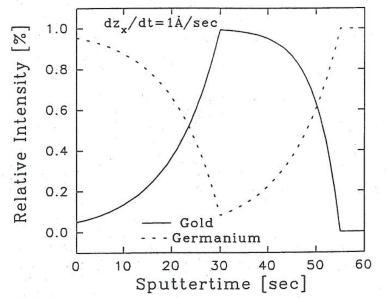
\includegraphics[scale=3.5]{figures/07_05.png}
	\caption{The relative intensity of gold from the sandwich as a function of sputter depth.}
	\label{fig:auint}
	\end{center}
\end{figure}

\subsection{Other Effects}
There are other effects leading both to broadening and shifts of the true profile which are not as easily dealt with. The sputtering process itself is quite a complex process and we shall here briefly mention a number of the effects that may lead to a broadening and introduce various errors when evaluating sputtering profiles.

\subsubsection{Statistical Broadening}
First of all the sputtering process is a random process, meaning that we should never expect to have a layer by layer removal. After some sputtering time we may have removed five layers off at one place of the surface, whereas seven layers have been removed at other places. This will lead to an additional broadening which is usually considered to be proportional to the square root of the depth in the region below \SI{100}{\angstrom}. For higher values of $z$, $\Delta z$ appears to saturate at roughly \SIrange{10}{20}{\angstrom}.

\subsubsection{Broadening by Surface Roughness}
Surface roughness will naturally also influence the resolution as will surface crystallography. Both effects can strongly influence the resolution as the sputter yield depends on the incoming angle of the ions. If for example a polycrystalline sample is sputtered for a long time, the sputtering itself may introduce structural changes of the surface leading to substantial broadening. This is clearly seen in \autoref{fig:emzi} where a polycrystalline zinc sample has been sputtered to a depth of \SIrange{3}{4}{\micro m} and subsequently studied by electron microscopy.

\begin{figure}[h!]
	\begin{center}
	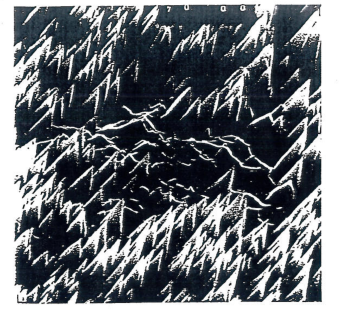
\includegraphics[scale=4]{figures/07_06.png}
	\caption{Electron microscope picture of a
 polycrystalline zinc sample sputtered to \SIrange{3}{4}{\micro m} depth.}
	\label{fig:emzi}
	\end{center}
\end{figure}

The surface which initially appeared flat is now extremely rough and it is clear that any concentration profiles measured on such a surface will be completely smeared out. This problem can to some extent be eliminated by averaging the incidence angle of the ion beam by rotating the sample during the sputtering process. The effect is shown in \autoref{fig:nicrsputter} where a sputter profile of a multi sandwich of Cr/Ni (each layer \SI{500}{\angstrom} thick) has been analysed with and without rotating the sample. The incident beam was \ce{Ar+} ions at \SI{1}{k\electronvolt} at an incidence angle of \ang{68} \cite{zalar}. The depth resolution for the rotated sample is clearly improved as seen in the lower panel of \autoref{fig:nicrsputter}.

\begin{figure}[h!]
	\begin{center}
	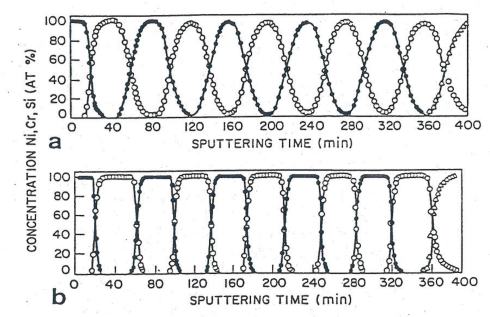
\includegraphics[scale=3.5]{figures/07_07.png}
	\caption{Sputter profile of a multi Ni/Cr sandwich without (top panel) and with (lower panel) simultaneous rotation of the sample.}
	\label{fig:nicrsputter}
	\end{center}
\end{figure}

\subsubsection{Preferential Sputtering}
If there is a large difference in sputter yield for the various components in the sample the surface concentration of the components may be changed due to the sputtering. Thus the surface composition will change from its true value to a composition determined by the steady state solution of the removal rates of the various components. This leads to an enrichment of the component which has the lower sputter yield and the sputter profiling will reflect a too high concentration of this particular component.

\subsubsection{Recoil Mixing}
The high energy ions hitting the surface will transfer energy and momentum to the surface atoms whereby there will be a mixing of the atoms at the surface. This in itself leads to a broadening of the profiles, but furthermore there will also be a possibility that some atoms are recoiled into the surface. This will result in a shift of the profiles to higher depths as some of the atoms are recoiled further into the sample before they are removed.

\subsubsection{Radiation Enhanced Diffusion and Segregation}
These effects both lead to broadening and errors in the concentration profiles. Due to the many defects the sputtering inevitably introduces in the surface region it will be much easier for the atoms to diffuse around. Thus if there is a component which has a very low surface energy, this component will prefer to segregate to the surface and cause an enrichment here which does not reflect the true composition of the sample. Similarly, any sharp interface will be smeared out by diffusion.

Several of the above effects will lead to broadening and as they all have to be convoluted it is appropriate to approximate the resolution function by a Gaussian

\begin{equation}
g(z-z\prime)=\frac{\pi \Delta z^2}{2}e^{-2\left(\dfrac{(z\prime-z)}{\Delta z}\right)^2}
\end{equation}

In general the resolution will decrease with depth as several of the discussed broadening effects are proportional to the depth sputtered. For a more detailed and rigorous treatment of the above discussed effects, the reader is referred to an excellent review by Hoffman \cite{hoffman} and references therein.

\section{Practical Sputter Profiling}
It is seen that there are many effects which make an accurate interpretation of a sputter profile a difficult task, even in cases where sandwiches of pure elements are studied. Sputter profiles are therefore generally presented as concentration profiles as a function of ion dosage. This is often sufficient as in many cases it is only necessary to discuss qualitative differences between different samples. In the following we shall go through a few such examples.

\subsection{Sputter Profile of Stainless Steel}
In \autoref{fig:sssputter} and \autoref{fig:ssheatsputter} the sputter profiles of a 18-8 stainless steel sample are shown just after it had been cut off a rod and after a heat treatment at \SI{600}{\degreeCelsius} for 600 seconds respectively.

\begin{figure}[h!]
	\begin{center}
	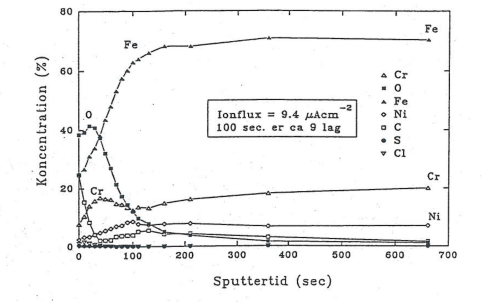
\includegraphics[scale=4]{figures/07_08.png}
	\caption{Sputter profile of stainless steel.}
	\label{fig:sssputter}
	\end{center}
\end{figure}

\begin{figure}[h!]
	\begin{center}
	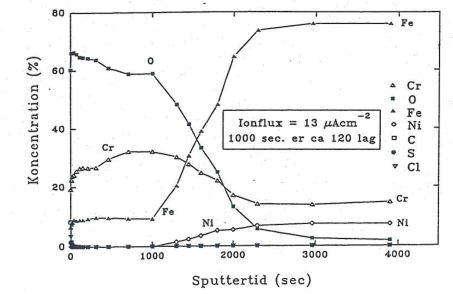
\includegraphics[scale=4]{figures/07_09.png}
	\caption{Sputter profile of heat treated
 stainless steel.}
	\label{fig:ssheatsputter}
	\end{center}
\end{figure}

In both cases a carbon contamination was observed at the surface prior to sputtering. Such a thin layer of surface contamination, is always observed on a sample that has been introduced into the apparatus from atmospheric pressure. It is readily removed after 10-20 seconds of sputtering. Also other forms of contamination like sulphur and chlorine can be observed. It is noticed that even on the non-treated surface (Fig. \ref{fig:sssputter}) there is a substantial oxide layer and an enrichment of chromium at the cost of iron and nickel in the surface region. This enrichment is further developed when the sample has been heated in atmospheric air at \SI{600}{\degreeCelsius} for 600 seconds as shown in \autoref{fig:ssheatsputter}. The surface layer can be identified by XPS as seen in \autoref{fig:ssxps} and consists mainly of \ce{Cr2O3} although less than \SI{10}{\percent} iron can still be observed.

\begin{figure}[h!]
	\begin{center}
	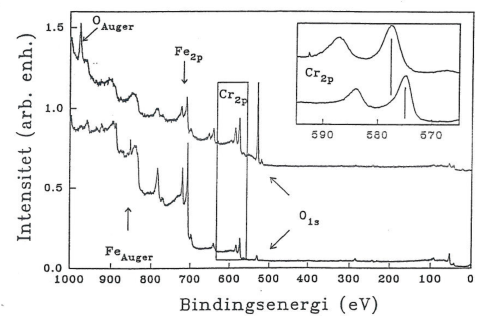
\includegraphics[scale=4]{figures/07_10.png}
	\caption{XPS spectra of the stainless steel sample before and after sputtering.}
	\label{fig:ssxps}
	\end{center}
\end{figure}

Approximately \SIrange{500}{1000}{\angstrom} must be removed before bulk values of the components are observed. The fact that it is chromium which is forming the protective oxide layer on the steel is in good agreement with the rule of thump that it is always the most reactive component which will segregate to the surface region and be oxidised. The reactivity of the transition metals is increasing from the right to the left. Therefore, if titanium had been present in the steel we would expect this to form an oxide overlayer as well. This simple picture holds well as long as the oxide layer grown is not too thick. For very thick layers (several \si{\micro m}) formed at high temperatures, the process becomes much more complex and NiO overlayers may be observed on top of the \ce{Cr2O3} \cite{alstrup}.

\subsection{Investigations of Electrical Contacts}
It has been mentioned that a substantial amount of all analysis performed by use of XPS and especially AES is done within the field of microelectronics. There are several problems which can be advantageously investigated with these methods and one of them is the formation of good contacts to the various semiconductors. Here we have chosen to show the contact formation to silicon. Gold usually forms good electrical contacts, but if it is deposited directly on the silicon it will readily diffuse into the silicon and be diluted. Therefore a layer of chromium is deposited on the silicon prior to the gold deposition. In \autoref{fig:aucrsisputter} the sputter profile of the contact is shown as deposited. In order to simulate ageing and use of the component it has been heated to \SI{300}{\degreeCelsius} for two hours and the result is shown in \autoref{fig:aucrsiheatsputter} where it is clearly seen that the chromium layer itself is not a sufficient diffusion barrier since silicon is observed in the gold overlayer and vice versa. If the procedure is repeated but the chromium is deposited in a background gas of nitrogen some chromium nitride will be formed as shown in \autoref{fig:aucrnsisputter}. Performing the same ageing experiment clearly shows (see Fig. \ref{fig:aucrnsiheatsputter}) that this construction is much better since the mixing has been minimised. Thus, the chromium nitride forms a diffusion barrier for gold and silicon.

\subsection{Control of Thin Coatings}
Coatings are used widely in industrial processes mainly for corrosion protection or for chemical inertness. In the latter case it is very common to deposit a thin layer of gold on the surface. For example many metals that are used for bijouterie and the rim of glasses will contain nickel. This is a highly non-desirable situation for metals in contact with the human body since it may cause allergic reactions. On the other hand, gold is a rather expensive material so the manufacturer wants to keep the layer as thin as possible. \autoref{fig:aunisputter} shows a sputter profile of a sample where the manufacturer was cutting the expenses too low since he was not successful in avoiding nickel at the surface. Only a few hundred \si{\angstrom} of gold had been deposited and since gold in this sort of industrial process is usually growing in an island growth mode, there will be areas free of gold exposing the nickel.

\begin{figure}[h!]
	\begin{center}
	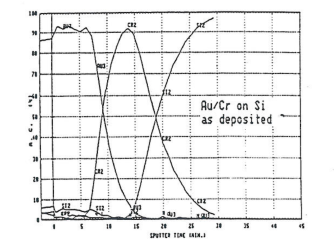
\includegraphics[scale=4.5]{figures/07_11a.png}
	\caption{Sputter profile of gold film on chromium on silicon as deposited.}
	\label{fig:aucrsisputter}
	\end{center}
\end{figure}

\begin{figure}[h!]
	\begin{center}
	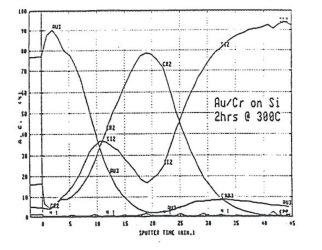
\includegraphics[scale=4.5]{figures/07_11b.png}
	\caption{Sputter profile of gold film on chromium on silicon heat treated to \SI{300}{\degreeCelsius} for two hours.}
	\label{fig:aucrsiheatsputter}
	\end{center}
\end{figure}

\begin{figure}[h!]
	\begin{center}
	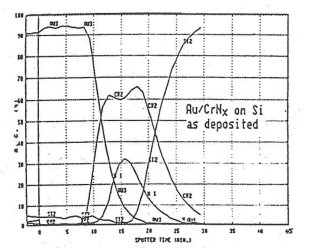
\includegraphics[scale=4.5]{figures/07_12a.png}
	\caption{Sputter profile of gold film on chromium-nitride on silicon as deposited.}
	\label{fig:aucrnsisputter}
	\end{center}
\end{figure}

\begin{figure}[h!]
	\begin{center}
	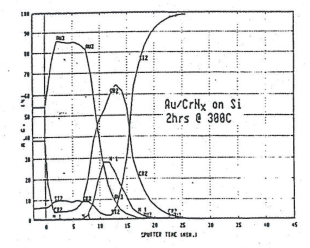
\includegraphics[scale=4.5]{figures/07_12b.png}
	\caption{Sputter profile of gold film on chromium-nitride on silicon heat treated to \SI{300}{\degreeCelsius} for two hours.}
	\label{fig:aucrnsiheatsputter}
	\end{center}
\end{figure}

\begin{figure}[h!]
 	\begin{center}
 	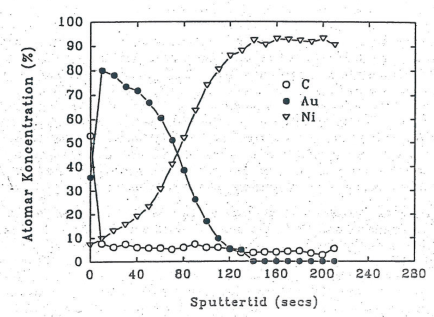
\includegraphics[scale=4]{figures/07_13.png}
 	\caption{Sputter profile of a glass rim consisting of nickel coated with gold.}
 	\label{fig:aunisputter}
 	\end{center}
\end{figure} 

\newpage
\section{Problems}
\begin{enumerate}
\item In the semiconductor industry it is often a requirement to be able to make good electrical contact to silicon wafers. This is often done by evaporating a thin film of gold upon the silicon. The evaporation rate is, however, in our case not known. The rate is, therefore, estimated by sputter profiling, that is measuring the surface composition while bombarding it with \SI{2.0}{k\electronvolt} Ar ions. The ion fluency is measured to be \SI{5}{\micro A/cm^2}. It takes 22 minutes before the gold disappears and the silicon appears. This is idealised, how does it look in reality?. The sputter yield has earlier been determined to be 2.6 Au atoms per Ar ion. Determine the thickness of the gold overlayer. How long time will it take to sputter through a silicon layer of a similar thickness when the sputter yield for Si is  $\sim$0.4? Which assumptions/complications must be considered using this method? Propose another and better method for determination of film thickness in this thickness regime.

\item Consider a sandwich structure consisting of a Si substrate on which one monolayer of Ge (\SI{2.5}{\angstrom}) has been deposited and then \SI{25}{\angstrom} Si on top. Finally the sandwich was terminated by another monolayer of Ge. All layers were grown epitaxially i.e. layer by layer. In order to test the process the sample was controlled by sputter profiling using AES. The Ge LMM (\SI{1147}{\electronvolt}), MVV (\SI{52}{\electronvolt}) Auger lines and the Si LVV (\SI{92}{\electronvolt}) are measured as a function of sputter time. In the following we will assume that the sputter process is ideal and removes the overlayer layer by layer (discuss the complications of sputter profiling). Show how the intensities of the Ge lines as well as the Si line develops with sputter time. Give the relevant equations and discuss the approximations. Which of the two Ge lines would you use in order to get a good quality control? Are there ways to improve the profile?
\end{enumerate}
 
%\newpage
\chapter{Vibrational Spectroscopies HREELS and IR}

Both the High Resolution Electron Energy Loss Spectroscopy (HREELS) and Infrared Adsorption Spectroscopy (IRAS) or just IR  rely on vibrational excitation of molecules adsorbed on the surface. HREELS can in general only be used on nice and plane single crystal surfaces under UHV conditions, whereas the IR method is much more applicable and can be used both on well defined surfaces (reflection IR) and on real catalysts (transmission IR and Diffuse Reflectance IR). It can even be used at relative high pressure, making it useful for investigating real catalyst {it in situ}. One of the advantages of using HREELS is that it can go to even very low frequencies meaning that energy losses due to phonons etc. can be investigated. The resolution in the IR experiments are usually much better than HREELS, but when molecules are adsorbed on surfaces the relaxation time is short due to the coupling  to the surface eliminating some of this advantage. For mor extensive treatment of these methods we shall here refer to \cite{Ibach,Ertl,Zangwill} 


\section{High Resolution Electron Energy Loss Spectroscopy}
\subsection{Experimental setup}

The HREELS experiments refers as the name says to high energy resolution since the energy loss spectroscopy also comes in a version where that is not the case. Earlier in chapter 3 we saw how electrons generated by an electron gun could be used to investigate the various energy losses mechanisms such as plasmon energy losses or losses by ionization. However, energy losses to vibrations and phonons are very small and cannot be observed if the energy distribution of the electrons is not very narrow say below 10 meV. The way to achieve monochromatized electron beams is by using low primary energies and then use an energy analyzer to select the appropriate energy. This is illustrated in figure 8.1.

\vspace*{11cm}

\noindent {\bf Figure 8.1} Schematic drawing of a HREELS experiment.

\vspace{1cm}

 The electrons are generated the usual way by heating a filament at a desired potential, the primary energy, which typically is less than 10 eV. The electrons are then energy analyzed by passing through an analyzer with an typical resolution between 1-5 meV and then  directed onto the sample. The electrons are interacting (reflected) by the sample and will in some cases also undergo an energy loss. The energy distribution of the reflected  is analyzed by a second analyzer which can be rotated around the specular direction. The experiment is not as easy to perform as those mentioned earlier. It is not trivial to get optimum resolution and at the same time a reasonable intensity. Also special precautions must be undertaken so that the slow electrons does not get detracted by any external fields, i.e. the setup must be screened from magnetic fields (also the earths field) by being incapsulated in a $\mu$-metal. The $\mu$-metal is a special alloy which leads the magnetic field lines in the metal screening the interior. Similarly are the electron beam also easily disturbed by changes in work function of the materials used in the analyzers. The inside of the analyzer is therefore  coated  with a graphite  ensuring an uniform work function.


\subsection{The energy loss spectrum}

 A typical HREEL spectrum is shown in Figure 8.2. At zero energy loss we find the elastically scattered electrons that have only been reflected from the surface. The overall resolution of the experiment is determined  by the FWHM of this elastic peak. The intensity of the energy losses are typically two orders of magnitude weaker much weaker and depends on the  nature of the excitation mechanism which can be  divided into dipole scattering and impact scattering.

\vspace*{11cm}

\noindent {\bf Figure 8.2} A HREEL spectrum of CO adsorbed on Ir(100). Notice that the resolution is below one meV. Taken from \cite{Bruckmann}
\vspace{1cm}

\subsubsection{Dipole scattering}
In this mechanism the electron is first of all reflected elastically by the surface leading to a high intensity of electrons in the specular direction. An electron approaching a metal surface will set up a time dependent  electrical field that will be screened by the metal surface so that  there is no field in the metal. This is described by a image charge with opposite sign traveling in the metal. The resulting electric field will be orthogonal to the surface and can be described in the frequency domain as 
\begin{equation}
E(t) = \int d\omega E(\omega)e^{-i\omega t}
\end{equation}
This electric field will thus contain frequency component equal to that of the vibrating molecule and  couple with any dynamical (time-dependent) dipole moment on the surface. Consider for example a CO molecule adsorbed standing on the surface. The  CO molecule is polarized and processes a very strong dynamical  dipole moment along the molecular axis. This dipole moment is further enhanced by the fact that the field from this dipole is screened by the metal resulting in mirror dipole with the same sign. The interaction Hamiltonian for this will naturally be
\begin{equation}
 {\bf H_{int}} \propto  \overrightarrow{E} \cdot \overrightarrow{\mu}
\end{equation} 
where $\overrightarrow{E}$  is the time-dependent electrical field from the electron and $\overrightarrow{\mu}$ is the  dipole moment operator for  the CO molecule. The probability for exciting the vibration of the molecule will then again be given by ``Fermi's golden rule'' where
\begin{equation}
P_{if}=|<\Psi_{i}|{\bf H_{int}}|\Psi_{f}>|^2
\end{equation}
Since the electron undergoing the elastic scattering on the surface is setting up the electric filed over a long range this energy loss may start happen already when the electron is far from the surface ( < 100 ANGSTROM). The inelastic scattering is predominantly a forward scattering so the change in momentum to reflect the electron is supplied by the substrate.

It is now obvious that there will be  a simple selection rule for the dipole scattering since vibrations involving dipoles parallel with the surface will be extinguished due to the metallic screening and no transitions will be possible. This is illustrated schematically in Figure 8.3

It is seen that the probability depends strongly on the size of the dipole. For example does CO have a strong dipole orthogonal to the surface when it is adsorbed in an up right position.  This makes it possible to measure  even remote amounts of CO (typically a few per mille of a monolayer) on a surface. Unfortunately is  the size of the dipole only constant in the low coverage regime. When the coverage increase the dipoles will start to interact  leading to screening and depolarization so the energy loss intensity is no longer simply  proportional to the coverage. 

\vspace*{11cm}

\noindent {\bf Figure 8.3} Schematic drawing of the selection rules for dipole scattering.

\vspace{1cm}
 

\subsubsection{Impact scattering}

In the case of impact scattering  short range interactions are involved taking  place when the electron interact with the potential of the atoms i.e. distances  of the order of 1 ANGSTROM.  In this case the electrons are scattered over a wide range of angles and are contrary to dipole scattering not directed in the specular direction. The mechanism for excitations are also very different and there are no simple selection rules like in the dipole scattering. This means that in principle, it is possible to measure the dipole forbidden energy losses. Unfortunately are the impact scattering in general rather weak and is most often only observed when going away from the specular direction. Here the dipole component dies of rather quickly whereas the impact scattering persists as mentioned above as it is much more isotropic. In this manner is it possible to distinguish  the two contributions from each other. It should for completeness also be mentioned that there is a third mechanism called ``Negative ion resonances''. Here the electron is captured in an orbital forming a shortlived negative intermediate losing energy before reemitted. 


\subsection{Experimental Results}

 The method can be used to identify unknown intermediates on a surface and in some cases also be used to investigate the orientation of the adsorbate and even at what sort of site it is adsorbed. For example was HREELS used to identify that formate is formed when  a Cu(100) crystal is exposed to several bars of CO$_{2}$ and H$_{2}$ at temperature below 363 K. The spectrum shows the energy losses characteristic for formate bound bidentate to the surface and the appropriate isotope shift for the C-H and C-D vibration was also found. The Spectra are shown in Figure 8.4. Please note that it is also possible for the electrons to gain energy from excited vibrations if the population is sufficiently high.



\vspace*{11cm}

\noindent {\bf Figure 8.4} The HREEL spectra of the intermediates formed by exposing a Cu(100) crystal to gas mixtures of  CO$_{2}$ + H$_{2}$ and  CO$_{2}$ + D$_{2}$ respectively. The energy losses are characteristic for formate and the C-H vibration undergoes the expected shift upon isotropical labeling. Taken from \cite{Formate}

\vspace{1cm}

Any gas phase molecule with N atoms  will have 3N degrees of freedom. Thus a CO molecule in the gas phase will have 6 degrees of freedom, 3 translatorial, two rotational, and one vibrational mode. When the molecule adsorbs on the surface the rotational and translational mode becomes converted into frustrated vibrational modes like 2 frustrated rotational modes and 3 frustrated translational modes. Of these modes is only the frustrated translational mode orthogonal to the surface, dipole active, whereas the other modes usually only have weak dipoles in the surface plane and therefore forbidden. The different modes for atomic hydrogen and CO adsorbed on a substrate is shown in Figure 8.5.

\vspace*{11cm}

\noindent {\bf Figure 8.5} The number of modes of atomic hydrogen and CO in different adsorption symmetries. Degenerate mode are shown next to each other \cite{Bradshaw}.

\vspace{1cm} 

 Thus only two energy losses should be expected for a CO molecule adsorbed standing up on the surface. These are observed at roughly 260 meV (C-O vibration) and at 60 mev (substrate-CO or frustrated translational mode) see Figure 8.2. (Simply divide by 8 for conversion from cm$_{-1}$ to meV). The other modes should in principle also be observable in the off-specular mode where impact scattering dominate, but they are weak and have low frequencies making them difficult to observe on the high background from the elastic peak. One example where the number of the dipole forbidden modes have been used to identify the bonding site is H on W \cite{Barnes} see figure 8.6. Here the vibration of the H atom normal to the surface is easily identified in specular scattering as  $\nu_1$. However when going away from the specular direction two other modes are  identified as the two translational frustrated modes along the surface. Since there are two and not one mode, which then would be degenerated, the H atom must be bridge bonded since an on top or a  four fold hollow site would lead to degeneration of $\nu_2$ and $\nu_3$. 



\vspace*{14cm}

\noindent {\bf Figure 8.6} HREEL spectra\\ of H-W(100)($\sqrt{2}x\sqrt{2}$)R45$^{\circ}$\\ measured with an electron\\ beam with primary energy\\ of 5.5 eV at 60$^{\circ}$ \cite{Barnes}.

\vspace{1cm} 

The size of the energy loss for a specific surface mode may also give information on the bonding site, although much care must be exercised here. According to Effective Medium Theory (EMT) will any adsorbate adsorb on a surface in a distance from the surface where it obtains its optimum electron density n$_{s}$. The binding energy will always have a minimum as a function of n$_{s}$ since at low electron density there are no overlap and thus no binding and at the very high electron density the Pauli repulsion takes over. Thus in this simple picture the bonding geometry only depends on n$_{s}$ and there will be no distinction between different adsorption sites like on-top, bridge or hollow sites. There are, however corrections to this model where the binding energy is  given by  

\begin{equation}
\Delta_{Bonding}=E(n_s) + E_{AS} + E_{1El}
\end{equation}

These correction terms determines where the adsorption will take place. The term E$_{AS}$, which is the Atomic Sphere correction, describes the repulsion occuring when to atoms comes close to each other. This means that it is in general most favorable for atoms to adsorb in high coordination sites since this gives the highest distance to the other atoms  minimizing the repulsion term when located in the optimum electron density. This explains why species like carbon, nitrogen, oxygen and sulphur usually are found in three or four fold hollow sites. When this is not the case it is due to the last  correction term, the one electron correction. 

\vspace*{13cm}

\noindent {\bf Figure 8.7} HREEL spectra of CO adsorbed on Ni(111) and Pt(111) \cite{Ibach}.

\vspace{1cm}
 

 Which trends can then be expected for atoms adsorbed in different sites on the surface. It is obvious that an atom sitting in a fourfold coordinated sites will feel a much slower variation in the electron density (and thus the resulting binding potential) as it vibrates orthogonal to the surface compared to an atom sitting for example in an  on top site. In the  latter case there will in principle  only be  one atom to supply the necessary electron density and as the electron density decays exponentially from the atom in the EMT will the potential vary much faster resulting in a steeper potential and thus in a higher frequency.  Thus the trends for vibration energies  predicted from this simple picture are hollow < bridge < on top adsorption sites.
An example of this behavior is shown in Figure 8.7 where the HREEL spectra of CO adsorbed on Ni(111) and Pt(111) are shown.  It is seen how the on top sites on Pt(111) leads to a significantly higher frequency for both the energy losses to CO.





\section{Infrared Adsorption Spectroscopy}

Infrared spectroscopy is well known from analysis of chemical compounds in the gas phase. It can also be used for studying adsorbates on solid surfaces. One way to this is very similar to the HREELS experiment where the infrared light is deflected from a plane surface for example a single crystal surface.  This method is referred to as Infrared Reflectance Adsorption Spectroscopy (IRAS) or (RAIRS) depending on where the infrared is put in. Here the light is send in nearly parallel to the surface and again only the components that are dipole active on the surface may adsorb the light. The reflected light is measured ad the absorbance can be measured. The advantage here is that it is possible to measure in a background of gas although care should be taken not to confuse gas phase adsorption  with adsorbate adsorbtion. 

The greatest advantage by IR  is that  it can be used to study real catalysts {\it in situ} in the transmission or reflectance mode. In the first case less than 0.1 g of catalysts is  pressed into a thin disk a few tenths of a mm thick. Transmission IR can then be used if the absorbance of the catalyst support material is low. This is typically the case when using oxides and considering wavenumber greater than 1000 cm$^{-1}$ which is equivalent to 125 meV. It is here also important that the size of the catalyst particles are smaller the wavelength of the infrared light since otherwise scattering would ruin the experiment. Often the absorbance of the catalyst itself make transmission impossible and then Diffuse Reflectance Infrared  Fourier Transform Spectroscopy (DRIFTS) may be used to measure the adsorbtion by surface species. Here the diffuse light scattered from a powder sample of catalyst is collected and analyzed. Just as in the transmission mode is the adsorbtion measured and it is in this manner possible to study different intermediates adsorbed on the catalyst while running a near realistic conditions taking the same precautions as mentioned above. By comparing observed absorbance bands to those measured on well defined surfaces is it possible to identify various species on the active catalyst. An important step towards closing the material gap. Figure 8.8 depicts a typical DRIFT spectrum of  methanol synthesis.




\vspace*{11cm}

\noindent {\bf Figure 8.8} DRIFT spectrum of a working methanol catalyst Cu/ZnO/Al$_{2}$O$_{3}$  in steady state at 30 bar and 413 K taken from \cite{Bailey}
\vspace{1cm} 

%\chapter{Low Energy Electron Diffraction LEED}
\section{Surface Crystallography}
Surface crystallography is just a special case of bulk crystallography where the crystal has been divided by a mathematical plane. We will only consider the terminology involving surfaces and some of the most often used concepts and encountered structures for metals namely Face Centered Cubic (FCC) Body Centered Cubic (BCC) and Hexagonal Close-Packed (HCP) lattices shown in \autoref{fig:unitcells}. For the more special structures like for instance the diamond structure we will refer to the literature \cite{Kittel, Ashcroft}.

\begin{figure}[h!]
	\begin{center}
	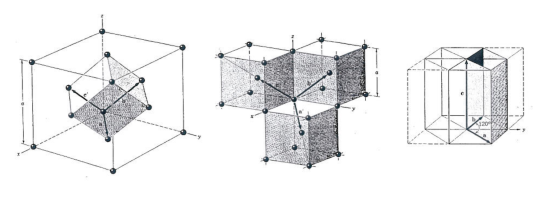
\includegraphics[scale=4]{figures/09_01.png}
	\caption{The unit cell for the FCC, BCC, and HPC lattices.}
	\label{fig:unitcells}
	\end{center}
\end{figure}

\subsection{Crystal Planes}
Since the surface structure and geometry is very important in many cases, for example when considering reactivity, and since it differs a lot from one surface structure to another it is important to have a notation that describes the various surfaces in a unique manner. The crystal surfaces are described by the vector normal to the surface given by

\begin{equation}
\vec{H}=h\vec{x}+k\vec{y}+l\vec{z}
\end{equation}

\noindent and the  notation is the name of the substrate and the surface normal vector $(hkl)$, for example Cu(100). Please note that the permutations Cu(100), Cu(010), and Cu(001) all describes the same surface as shown in \autoref{fig:basalplanes} for the cubic crystals. Negative numbers are noted by a bar over the number so Cu(100) is naturally equal Cu(0$\overline{1}$0). The three basal planes for the cubic crystals are (100), (110) and the (111). The respective cuts are shown in \autoref{fig:basalplanes} and the relative positions of the surface atoms are shown in \autoref{fig:surfaces}.

\begin{figure}[h!]
	\begin{center}
	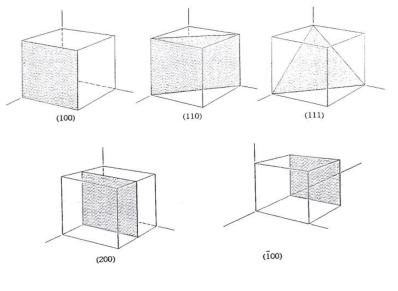
\includegraphics[scale=4]{figures/09_02.png}
	\caption{The basal planes formed by cuts of the unit cells of the simple crystal structures.}
	\label{fig:basalplanes}
	\end{center}
\end{figure}

An important parameter for surfaces are often the density of atoms in the surface. Note that for FCC crystals the (110) is the most open whereas the (111) is the most close packed. For BCC crystals it is the opposite order i.e. the (111) most open and (110) most close packed. Also more complicated surface structures containing steps or even kinks may be described in this notation as $n(h_tk_tl_t)\times(h_sk_sl_s)$ where $n$ describes that the surface contains $n$ rows of atoms forming a terrace of $(h_tk_tl_t)$ and one step of type $(h_sk_sl_s)$. Thus a (775) surface is equivalent to $6(111)\times(11\overline{1})$. In this manner all sorts of surfaces may be constructed, but the question is naturally whether they are stable or will facet into other structures.

\begin{figure}[h!]
	\begin{center}
	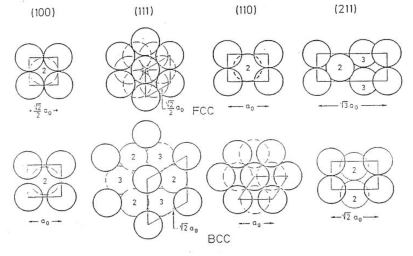
\includegraphics[scale=4]{figures/09_03.png}
	\caption{The surface structures of the basal planes for the FCC and BCC.}
	\label{fig:surfaces}
	\end{center}
\end{figure}

A particular surface structure may be prepared by spark cutting a single crystal normal to the desired direction. The crystal is usually oriented by Laue X-ray diffraction with an accuracy better than \ang{0.5}. The surface is then polished with polish paste with decreasing grain size until all scratches etc. are removed and a mirror like surface is obtained. Sometimes, in particular for the soft materials like Cu, an additional electro polish is needed to remove damaged layers. Finally the crystal is mounted in the UHV chamber and is cleaned by repeated cycles of sputtering and annealing. Getting a clean single crystal surface may be tedious work and may take several months. The cleaning procedure varies from element to element and usually effective and successful recipes can be found in the literature.

\subsection{Adsorbate Sites}
The definition of the most frequent  adsorption sites are shown in \autoref{fig:adsorptionsites}. They are named on-top site, bridge sites  (may be long or short bridged), and hollow sites which may be three fold hollow or four fold hollow. In for example the FCC(111) cases it is also necessary to distinguish between HCP and FCC sites describing whether there is an atom just below the site or it is in the second layer.

\begin{figure}[h!]
	\begin{center}
	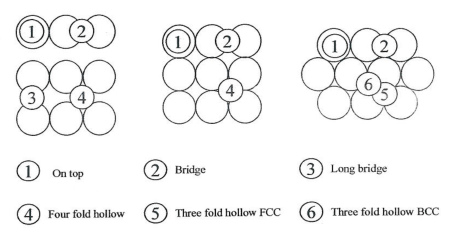
\includegraphics[scale=3.5]{figures/09_04.png}
	\caption{The adsorption sites for various surface geometries.}
	\label{fig:adsorptionsites}
	\end{center}
\end{figure}

\subsection{The Two-Dimensional Lattice}
A two-dimensional structure processing periodicity can be described by a two dimensional lattice. Any point in this lattice can be reached by a suitable combination of basis vectors. Two unit vectors will describe the smallest cell in which an identical arrangement of the atoms is found. The whole lattice can then be described by moving this unit cell by any linear combination of the unit vectors. These vectors form the {\it Bravais} lattice which is the set of vectors by which all points in the lattice can be reached.

\section{Low Electron Energy Diffraction}
\subsection{Experimental Set-up}
Having defined the fundamental structure we will now turn to the Low Electron Energy Diffraction Experiment (LEED). The first experiment made realising that electrons could be used for investigating surface structures was made by Davidson and Germer in 1927 \cite{Davidson}, but as the crystals could not be kept clean (due to poor vacuum) it was not until the late sixties that the method started to take off. Several excellent reviews and monographs have been written on this subject \cite{Pendry, Hove, Heinz, Ertl}. The experiment relies on the duality of electrons which in some case should be considered as particles and under other conditions as wave packets. If we choose to use electrons with energy around the minimum in the universal curve (Fig. \ref{fig:mean_free_path}) (\SIrange{40}{200}{\electronvolt}) where we have the maximum surface sensitivity the wavelength of the electrons will be comparable with the lattice distance of single crystals considered here.

\begin{eqnarray}
\lambda	& =	& \frac{h}{p}\\
p	& =	& \hbar k=\sqrt{2mE_p}\\
\lambda(\si{\angstrom})	& =	& \sqrt{\frac{150.4}{E_p(\si{eV})}}
\end{eqnarray}

This means that the electrons may be scattered elastically  in the surface and undergo constructive and destructive interference. The back scattered electrons are then analysed and from that the symmetry of the surface may be deduced.

The experimental set-up is shown in \autoref{fig:leed}.  A beam of electrons with energy $E_p$ from a relative simple electron gun mounted in the center of the LEED optics is directed towards the surface. The crystal is mounted so it can be positioned in the center of three concentric hemispherical grids. The inner grid is grounded whereas the middle grid is kept on a negative potential slightly below $E_p$ so only electrons which have not undergone any energy losses are allowed to pass. Between the last grid and an outer fluorescent screen there are a potential difference between \SIrange{2}{5}{kV} so the electrons that pass are accelerated towards the fluorescent screen where they will form observable spots. The screen is  transparent so the spots can be observed from behind it as well without being obstructed by the sample mount. The spots can then be photographed or followed by a CCD camera. More elaborate set-ups have been constructed for Spot Profile Analysis LEED (SPALEED) where the detailed profile can reveal details on the long range structure, but that will not be considered here.

\begin{figure}[h!]
	\begin{center}
	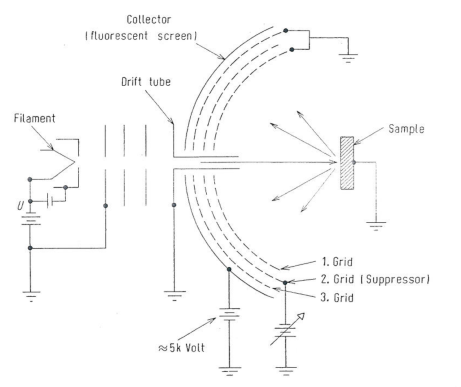
\includegraphics[scale=4]{figures/09_05.png}
	\caption{Schematic drawing of LEED optics.}
	\label{fig:leed}
	\end{center}
\end{figure}

\begin{figure}[h!]
	\begin{center}
	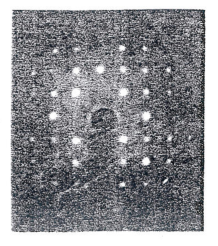
\includegraphics[scale=4]{figures/09_06.png}
	\caption{LEED pattern obtained from a Cu(100) surface reconstructed by adsorption of atomic hydrogen. The energy of the electrons was relatively high $E_p=\SI{178}{\electronvolt}$ and the beam was  normal to the surface. Only the bright spots are observed on a clean Cu(100). From \cite{HonCu}.}
	\label{fig:culeed}
	\end{center}
\end{figure}

Such a LEED pattern is reproduced in \autoref{fig:culeed} \cite{HonCu}.

The principle of the experiment is shown schematically in \autoref{fig:leedsketch} where an incoming electron beam interacts with a crystal described by $\vec{a_1}$ and $\vec{a_2}$. The (00) beam is reflected directly back into the electron gun and can therefore not be observed unless  the crystal is tilted.

The intensity of the spots formed on the screen can also be followed as a function of primary energy $E_p$. The spots will move towards the zero order spot with increasing energy and then varying strongly in intensity. The diffraction in the two-dimensional lattice lead to the diffracted beams indicated in \autoref{fig:leedsketch} whereas the $d$ modulation of the intensity as a function of $E_p$ is due to diffraction between subsequent layers into the crystal. We will first concentrate on understanding the diffraction pattern which reveals the two-dimensional symmetry of the surface layers and in the end of this chapter  briefly touch upon the intensity variation, which can be used to determine the distances in the surface structure.

\begin{figure}[h!]
	\begin{center}
	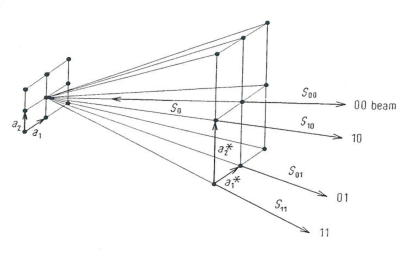
\includegraphics[scale=4]{figures/09_07.png}
	\caption{Sketch of the LEED experiment on a single crystal spanned by $\vec{a_1}$ and $\vec{a_2}$.}
	\label{fig:leedsketch}
	\end{center}
\end{figure}

\subsection{Kinematic Theory}
The direction of the diffraction beams can be found by first considering what happens when an electron interacts with  atoms in the surface. The differential scattering cross section for an elastic collision of an electron with a fixed atom is given by the asymptotic solution to the Schr\"{o}dinger equation:

\begin{equation}
\frac{-\hbar^2}{2m}\nabla^2\Psi +V\Psi =E\Psi
\end{equation}

Far away from the atom $V=0$ and the asymptotic solution to $\Psi$ can be written as a sum of an incoming plane wave and an outgoing spherical wave:

\begin{equation}
\Psi =e^{i\vec{k}\vec{r}}+f(\alpha,\phi)\frac{e^{i\vec{k}\vec{r}}}{\vec{r}}
\end{equation}

\noindent where $f(\alpha,\phi)$ is the amplitude of the outgoing electron and $\vert f(\alpha,\phi)\vert^2$ is the differential scattering cross section which must be found by solving the Schr\"{o}dinger equation in the vicinity of the atom where $V\neq 0$. $\alpha$ and $\phi$ are the angles of the scattering. Assuming that the potential is spherically symmetrical the solutions to the Schr\"{o}dinger equations are separable in the coordinates $r, \alpha, \phi$ and the wave functions are of the hydrogen type namely a product of radial and spherical harmonic:

\begin{equation}
\Psi_n(r,\alpha,\phi)=R_n(r)\Upsilon_{l,m}(\alpha,\phi) 
\end{equation}

\noindent where $n, l$ and $m$ are the principal, azimuthal and magnetic quantum numbers, respectively.

The amplitude of the scattered electrons can  be described as an expansion of phase shifted Legendre polynomials where the phase shift comes from the interaction with the potential $V$. Usually a band structure potential have been used for $V$ when describing atoms in a solid. For details on scattering of electrons on potentials we will refer to standard quantum mechanics \cite{Shiff,Merzbacher}.

What happens when considering more than one  atom scattering the incoming electrons? Firstly, consider a plane wave scattering on two atoms separated by a distance of $R$. This would lead to two spherical waves interfering at the position of the observer (see Fig. \ref{fig:electronscatter}). The difference in phase of the two waves $\Delta$ is given by

\begin{figure}[h!]
	\begin{center}
	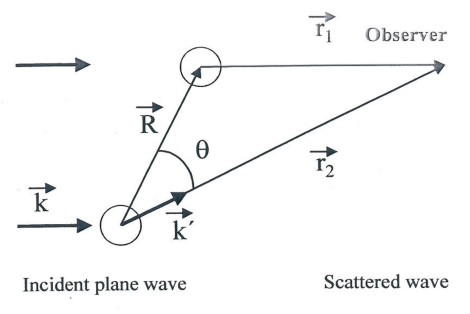
\includegraphics[scale=2]{figures/09_08.png}
	\caption{An incoming electron with wave vector $\vec{k}$ scatters on two atoms with distance $\vec{R}$.}
	\label{fig:electronscatter}
	\end{center}
\end{figure}

\begin{equation}
\Delta=e^{i\vec{k} \vec{R}+i\vec{k} \vec{r_1}-i\vec{k'}\vec{r_2}} 
\end{equation}

If the observer is far away, which is always the case here, then $\vec{r_1}\approx\vec{r_2}\gg \vec{R}$ leading to $r_2\approx r_1+R\cos(\theta)$, thus

\begin{eqnarray}
\Delta	& =		& e^{i\vec{k}\vec{R}+ik_xr_1-ik'_x(r_1+R\cos\theta)+ik'_yR\sin\theta)}\\ 
\Delta	& \approx	& e^{i\vec{k}\vec{R}-ik'_x(R\cos\theta)+ik'_yR\sin\theta} \mbox{, Since } k_x\approx k'_x\\
\Delta	& \approx	& e^{i\vec{k}\vec{R}-i\vec{k'}\vec{R}}=e^{i(\vec{k}-\vec{k'})\vec{R}}=e^{i\vec{\Delta k}\vec{R}}
\end{eqnarray}

\noindent where $\vec{k^\prime}$ is parallel to $\vec{r_2}$ and  $\vec{\Delta k}$ is the difference between $\vec{k}$ and $\vec{k^\prime}$.

The amplitude of the wave seen by the observer will be  proportional to the phase difference. If we now turn to a unit cell which may contain several different atoms the amplitude from this  $F(\Delta k)$ can be found by summing over the contributions from the $i$'th atom in the unit cell as

\begin{equation}
F(\vec{\Delta k})=\sum_i f_i(\vec{\Delta k})e^{i\vec{r_i}\vec{\Delta k}}
\end{equation}

\noindent where $f_i$ is the so called "form factor" which is dependent on the potential for the various atoms.

Let us now consider a two-dimensional lattice described by the vectors $\vec{a_1}$ and $\vec{a_2}$ as shown in \autoref{fig:leedsketch}. The crystal is considered to be finite and consisting of $M$ atoms in the $\vec{a_1}$ direction and $N$ in the $\vec{a_2}$ direction.

The amplitude $\Delta(\vec{\Delta k})$ from this plane can be found by summing over all the phase differences between the electrons scattered on each unit cell leading to:

\begin{equation}
\Delta(\vec{\Delta k})=F(\vec{\Delta k})\sum_{m=0}^{M-1}e^{im\vec{a_1}\vec{\Delta k}}\sum_{n=0}^{N-1}e^{in\vec{a_2}\vec{\Delta k}}
\end{equation}

Remembering that

\begin{equation}
\sum_{m=0}^{M-1}x^m=\frac{1-x^M}{1-x}
\end{equation}

\begin{equation}
\Delta(\vec{\Delta k})=F(\vec{\Delta k})\frac{(1-e^{iM\vec{a_1}\vec{\Delta k}})(1-e^{iN\vec{a_2}\vec{\Delta k}})}{(1-e^{i\vec{a_1}\vec{\Delta k}})(1-e^{i\vec{a_2}\vec{\Delta k}})}
\end{equation}

It is not the amplitude but the intensity which is interesting so we would have to multiply the amplitude by its complex conjugate and by using the cosine relations we find

\begin{equation}
I(\Delta \vec{k}) = \frac{\sin^2\left(\frac{M}{2}\vec{a}_1 \Delta k_{\parallel}\right) \sin^2\left(\frac{N}{2}\vec{a}_2 \Delta k_{\parallel}\right)}{\sin^2\left(\frac{1}{2}\vec{a}_1 \Delta k_{\parallel}\right) \sin^2\left(\frac{1}{2}\vec{a}_2 \Delta k_{\parallel}\right)}
\end{equation}

\noindent since $\vec{a_1}\vec{\Delta k}=\vec{a_1}\vec{\Delta k_{\parallel}}$ as $\vec{a_1}$ is located in the surface plane.

Now it is possible to see that there will only be an intensity in specific directions namely when the denominator goes towards zero i.e. when:

\begin{eqnarray}
\vec{a_1}\vec{\Delta k_{\parallel}}	& =	& h2\pi \\
\vec{a_2}\vec{\Delta k_{\parallel}} & =	& l2\pi \\
h,l	& \in	& Z
\end{eqnarray}

Thus for a plane of sufficient dimensions and when the observer is far away from the plane the spherical waves scattered from each unit cell will give rise to localised beams diffracted in directions parallel to the surface so they obey the above relations characterised by the indices $h$ and $l$.

\subsubsection{The Reciprocal Lattice}
When having a real-space lattice defined as above where for example

\begin{equation}
\vec{r_{m,n}}=m\vec{a_1}+n\vec{a_2}
\end{equation}

\noindent it is possible to define a reciprocal lattice vector in the plane given by

\begin{equation}
\vec{g_{h,l}}\equiv h\vec{a_1^*}+l\vec{a_2^*}
\end{equation}

\noindent where the basis vectors of the reciprocal lattice are defined as:

\begin{eqnarray}
\vec{a_1^*}	& \equiv	& 2\pi\frac{\vec{a_2}\times\vec{z}}{\vec{a_1}\cdot\vec{a_2}\times\vec{z}}\\
\vec{a_2^*}	& \equiv	& 2\pi\frac{\vec{z}\times\vec{a_1}}{\vec{a_1}\cdot\vec{a_2}\times\vec{z}}
\end{eqnarray}

\noindent where $\vec{z}$ is the vector normal to the surface and the denominator is the volume of the unit cell. 

\begin{equation}
\vec{\Delta k_{\parallel}}=\vec{g_{h,l}}
\end{equation}

This means the diffracted beam occurs when the change in momentum parallel to the surface equals a reciprocal vector or linear combination thereof. Let us try to relate this information to the spot we see on our screen. That we have a spot means that a diffracted beam $(h,l)$ crosses our LEED optics as shown in \autoref{fig:leedcs}. In a conventional LEED optic the radius of the screen $R$ is known. By observing the position of the spot we can thus determine the angle $\theta_{h,l}$ the diffracted beam has been scattered.

\begin{figure}[h!]
	\begin{center}
	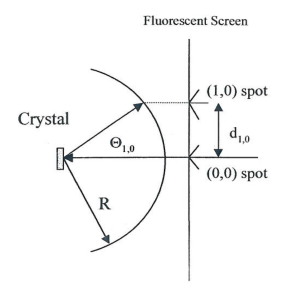
\includegraphics[scale=4]{figures/09_09.png}
	\caption{Cross section of the experimental set-up. Radius of the screen is $R$ and the beam $(h,l)$ gives a spot a distance $d_{h,l}$ measured from the zeroth order spot.}
	\label{fig:leedcs}
	\end{center}
\end{figure}

\begin{equation}
\sin{\theta_{h,l}} = \frac{d_{h,l}}{R} = \frac{g_{h,l}}{k}
\end{equation}

\noindent where $k$ is the wave vector of the electron. (We are assuming normal incidence of the incoming beam. This is not a necessity, but simplifies the experiment). It is seen that the distance seen on the screen $d_{h,l}$ is inversely proportional to the  square root of the energy, meaning that all spots will converge towards the zeroth order spot for high energies as mentioned earlier. This is a good method for identifying  the zeroth order spot. It is also possible to give an estimate of the lattice distance of the crystal by measuring the distance $d_{1,0}$, which is between the first order spot $(1,0)$ and the zeroth order spot $(0,0)$. Since $g_{1,0}=2\pi/a_1$ the lattice distance is given by:

\begin{equation}
a_1=\frac{2\pi R\hbar}{d_{1,0}\sqrt{2mE_p}}
\end{equation}

Since the spots are usually not extremely sharp this is not a very accurate method for determining lattice distances.

\subsubsection{The Coherence Length}
The diameter of the spot seen on the screen depends critically on the level of order on the surface, the quality of the electron beam used and the temperature of the crystal. Let us first assume that we have an ideal electron beam i.e. the electron trajectories are all parallel and the beam is monochromatised. If we look at a spot profile the intensity will be given by:

\begin{equation}
I\left(\vec{\Delta k}\right)=\frac{\sin^2\left(M/2 \vec{a_1}\vec{\Delta k_{\parallel}}\right)}{\sin^2\left(1/2\vec{a_1}\vec{\Delta k_{\parallel}}\right)}
\end{equation}

\noindent which can be approximated as

\begin{equation}
I(x)\propto\frac{\sin^2(x)}{x^2}
\end{equation}

\noindent where $x=M/2\vec{a_1}\vec{\Delta k_{\parallel}}$ and the intensity profile is shown in \autoref{fig:spotprofileint}.

\begin{figure}[h!]
	\begin{center}
	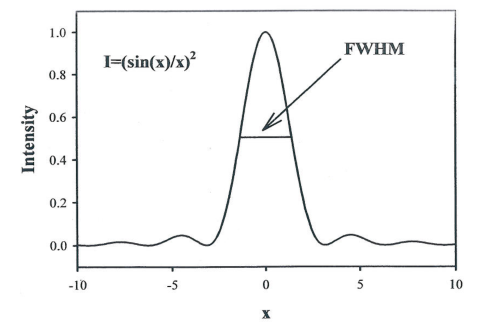
\includegraphics[scale=3]{figures/09_10.png}
	\caption{The intensity of the spot profile as a function of $x$ as defined in the text.}
	\label{fig:spotprofileint}
	\end{center}
\end{figure}

It can be shown that the FWHM of the spot is given by $\vec{a_1}\vec{\Delta k_{\parallel}}=0.44\pi /M$ meaning that if there are just ordered areas bigger than, say, 30 by 30 atoms this effect will no longer contribute significantly  to the  broadening of the observed spots. Thus LEED is not very useful for determining the over all order of a surface since it only reflects the areas that are ordered and discriminates those which are disordered. If one however observes a LEED pattern with diffuse spots the surface order is certainly of poor quality.

Usually it is the quality of the electron gun that sets the limit of how sharp the spots can be. The beam diameter will normally be of the order of \SIrange{0.1}{1.0}{mm}, which is the area the LEED experiment is probing. Unfortunately the beam energy is not monochromatised and completely parallel. The energy resolution is as we shall see of less importance, but both effects contributes to an uncertainty of the parallel momentum $\Delta \Delta k_{\parallel}$  of the incoming beam, which will be reflected in the outgoing beams. This uncertainty in the beam can be translated into a transfer width $W$ given by

\begin{equation}
W=\frac{2\pi}{\Delta \Delta k_{\parallel}}
\end{equation}
 
\noindent where

\begin{equation}
\Delta k_{\parallel}=2\pi\sqrt{\frac{E_p}{150.4}}(\sin(\theta_{out})-\sin(\theta_{in}))
\end{equation} 

By neglecting contributions from $\theta_{out}$ and assuming normal incidence we find the respective uncertainties for divergence and energy by differentiation. From those we can estimate the respective transfer widths to:

\begin{equation}
W_{\theta_{in}}=\frac{\lambda}{\cos(\theta_{in})\Delta\theta_{in}}
\end{equation}

\noindent and 

\begin{equation}
W_{E_p}=\frac{4\pi E_p}{\Delta k_{\parallel}\Delta E_p}
\end{equation}

Substituting realistic values for a conventional LEED system like $E_p=\SI{100}{\electronvolt}$, $\Delta E_p=\SI{0.5}{\electronvolt}$, $\Delta\theta_{in}=\ang{0.6}$ and $2\pi /\Delta k_{\parallel}=\SI{2.5}{\angstrom}$ we get $W_{\theta}=\SI{100}{\angstrom}$ and $W_E=\SI{1000}{\angstrom}$. It is obvious that the uncertainty of the beam convergence is dominating meaning that as long as we have ordered islands on the surface that are larger than the transfer width of our LEED optics we will not be able to notice an effect on the sharpness of the spots. Normally we are talking about a coherence length on the order of \SIrange{100}{200}{\angstrom} meaning that we can have a crystal which in LEED will appear well ordered, but locally may have areas that are completely disordered. This may first be realised when Scanning Tunneling Microscopy (STM) experiments are performed since that method is very sensitive to the local order. By optimising the experimental set-up it is possible to obtain electron beams in which the electron trajectories are parallel to a high degree. In this manner the uncertainty of the angle can be eliminated and long range order may be observed. The detail are investigated by spot profile analysis and referred to as SPALEED. The experiment requires dedicated equipment and is commercially available.

For completeness it should also be mentioned that the temperature of the sample have a profound effect on the spot profile since the atoms in the surface oscillates due to the phonons. This gives an uncertainty of the positions of the surface atoms which will naturally result in a decreasing intensity and broadening of the LEED spots. Thus it is preferable to stay at room temperature or lower when doing LEED experiments.The intensity is given by:

\begin{equation}
I=I_0e^{-2M}
\end{equation}

\noindent where

\begin{equation}
2M=\frac{12h^2T}{mk_B\theta_D^2}\left(\frac{\cos(\phi)}{\lambda}\right)^2
\end{equation}

\noindent where $\phi$ is the scattering angle, $\lambda$ is the wavelength, and $\theta_D$ is the Debye temperature. By plotting $\log{I}$ vs. temperature the Debye temperature can be extracted. At low mean free paths it will primarily be the Debye temperature of the surface layer which is lower than that of the bulk.

\subsection{Multiple Scattering}
Above we have only considered one plane of atoms but the scattering process will in general always take place in several non-equivalent layers. This is the effect that will cause modulation of the diffracted beam as mentioned earlier leading to the IV-curves. A first glance one could expect the resulting LEED patterns just to be a sum of the scattering in the different non-equivalent planes. This would be the case if the electrons were only scattered once, but that is not the case since the cross section for scattering is rather large. Electrons scattered in the second layer may also be scattered in the first layer and vice versa leading to a convolution of the diffraction. The resulting LEED patterns must therefore be found by determining the {\emph coincidence lattice} which is the lattice formed by all the non-equivalent layers. I.e. when determining the unit cell of the adsorbate and the substrate one must find the unit cell that repeats the symmetry of both. We shall look at an example later to demonstrate this principle.

\subsection{Notation and Examples}
In the following will first look at the notation for the different surface structures and then give some examples.

As we have seen a real space surface lattice in a LEED experiment will be reflected as a reciprocal lattice on the LEED screen. We can say that the LEED pattern is just a Fourier transform of the real space lattice. Starting out with the  simple basal planes the respective LEED patterns are found by finding the respective reciprocal lattice vectors. This is the typical starting situation when doing experiments where the first LEED pattern is obtained in order to check the structure and  to some extend the quality of the crystal. This pattern is referred to as the $1\times 1$ structure. Now lets consider what happens if we adsorb 0.25 monolayer of sulphur on for example a Ni(100) surface. The sulphur is known to prefer four fold hollow sites as indicated in the real space model shown in \autoref{fig:snileed}. The new unit vectors in real space will be the same as those of the Ni(100) substrate except that they are twice as long. The respective LEED pattern is found by finding the  respective reciprocal basis vectors using the formulas above. Since the new basis vectors was twice as long in real space they will now be half as long in reciprocal space leading four times as many spots in the respective LEED pattern.

\begin{figure}[h!]
	\begin{center}
	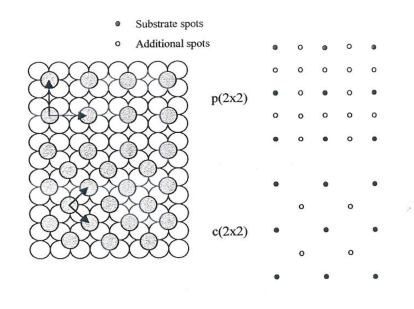
\includegraphics[scale=4]{figures/09_11.png}
	\caption{A real space model of a quarter and a half monolayer of sulphur adsorbed on Ni(100) and the respective LEED pattern.}
	\label{fig:snileed}
	\end{center}
\end{figure}

\subsubsection{Woods Notation}
Assume that the substrate is described by the basis vectors $\vec{a_1}$ and $\vec{a_2}$. The new basis vectors describing the surface structure are then $\vec{b_1}$ and  $\vec{b_2}$. In Woods notation this is described as S-Ni(100) $(\vec{b_1}/\vec{a_1}\times\vec{b_2}\vec{a_2})R\theta^{\circ}$ telling us that it is a $2\times 2$ structure of sulphur on  Ni(100) rotated $\theta$ degrees. Woods notation is quite convenient, but cannot be used to describe all LEED structures. When the angle between the new basis vectors in real space is changed with respect to the angle between the  substrate vectors the notation is no longer valid and we must use the matrix notation which is always valid.

\subsubsection{The Matrix Notation}
The substrate is in real space represented by a matrix:

\begin{equation}
{\bf A}=\begin{pmatrix}
a_{11}	& a_{12}	\\
a_{21}	& a_{22}
\end{pmatrix}
\end{equation}

Similarly the new basis set can be described by the matrix:

\begin{equation}
{\bf B}=\begin{pmatrix}
b_{11}	& b_{12}	\\
b_{21}	& b_{22}
\end{pmatrix}
\end{equation}

We can now find the matrix {\bf G} which maps {\bf A} on {\bf B}

\begin{equation}
{\bf B}={\bf GA}
\end{equation}

\noindent which is the one used in matrix notation i.e. S-Ni(100) $\left(\begin{smallmatrix} g_{11}	& g_{12}	\\ g_{21}	& g_{22 }\end{smallmatrix}\right)$, which in this specific case gives S-Ni(100) $\left(\begin{smallmatrix} 2	& 0	\\ 0	& 2 \end{smallmatrix}\right)$. Please note that the same set of equations also applies for the reciprocal set of vectors i.e.

\begin{equation}
{\bf B^*}={\bf G^*A^*}
\end{equation}

In many cases it is convenient to determine ${\bf G^*}$ from the LEED pattern and then find $\vec{b_1}$ and $\vec{b_2}$ in terms of $\vec{a_1}$ and $\vec{a_2}$ by the relation

\begin{equation}
{\bf G}=(({\bf G^*})^{\mathrm{T}})^{-1}
\end{equation}

The area of the new unit cell is conveniently found as $\det({\bf G})$.

The various types of overlayer structures can be classified by {\bf G}, but that is beyond the scope of these notes and we will refer to for example \cite{Ertl, woodruff} for details.

\subsubsection{Other Examples}
Now we have the machinery ready for investigating surface structures. If we reconsider the structure above with sulphur on Ni(100) and add another quarter of a monolayer the center positions will also be occupied. The first LEED structure is often called a p$(2\times 2)$ structure while the second is called a c$(2\times 2)$ - p for primitive $2\times 2$ and c for centred $2\times 2$. The correct notation for the latter is in Woods notation S-Ni(100)($\sqrt{2}\times \sqrt{2})R\ang{45}$ or in the matrix notation S-Ni(100) $\left(\begin{smallmatrix} 1	& 1	\\ -1	& 1 \end{smallmatrix}\right)$, since this cell is smaller than the $2\times 2$. In the above examples the adsorbate lattice automatically also included the substrate lattice. Let us now look at an example where we need to look for a coincidence cell as mentioned earlier. Consider a Ni(110) surface and the respective LEED structure when oxygen is added as shown in \autoref{fig:onileed}.

\begin{figure}[h!]
	\begin{center}
	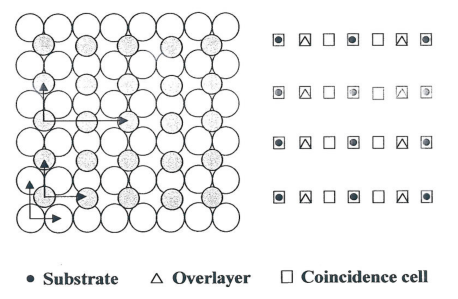
\includegraphics[scale=4]{figures/09_12.png}
	\caption{The real space model and the respective LEED patterns for the substrate, the overlayer, and the coincidence cell for oxygen on Ni(110).}
	\label{fig:onileed}
	\end{center}
\end{figure}

Let us assume that 2/3 of a monolayer oxygen has been adsorbed and that the oxygen is sitting in two non-equivalent positions. The LEED pattern from the substrate is indicated as dots. The LEED pattern from the oxygen overlayer is indicated as triangles, whereas the spots occurring from the coincidence cell is shown as open squares. Please note that the correct LEED pattern is not just the sum of the substrate and the overlayer diffraction pattern, but that the coincidence cell which describes both at the same time must be found in order to determine the correct pattern.

The LEED pattern only gives us the size and orientation of the new unit cell  formed by the substrate and the adsorbate together. It is not possible to say anything about the actual binding site or coverage of the adsorbate from the LEED pattern alone. (The adsorbate layer can be shifted in the unit cell of the substrate without any consequence for the resulting LEED pattern.) This must be determined from other experiments such as XPS and AES concerning the coverage and HREELS, STM and UPS concerning the actual binding site.

\subsection{Domains}

\begin{figure}[h!]
	\begin{center}
	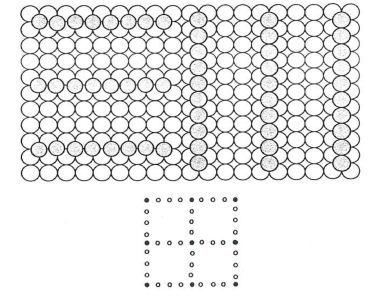
\includegraphics[scale=4]{figures/09_13.png}
	\caption{The real space model for two different domains of $4\times 1$ structure on Ni(100). The respective LEED pattern shows the result of both types of domains present on the surface.}
	\label{fig:41nileed}
	\end{center}
\end{figure}

Yet another effect may complicate the analysis of LEED patterns namely \emph{domains}. Remember that in a typical LEED experiment the electron beam probes an area of a diameter of \SIrange{0.1}{1.0}{mm} and that if we just have islands which are larger than the transfer width then we will obtain nice LEED patterns from these islands (the intensity naturally being proportional to the coverage of these islands). Due to the surface symmetry these islands may differ in orientation. Consider for example a simple $4\times 1$ structure on Ni(100) as shown in \autoref{fig:41nileed}. When this structure nucleate there will be two equal possibilities of orienting the island on a (100) surface. As we will be sampling over many islands that are randomly oriented in two-dimensions the resulting LEED pattern will simply be the sum of the LEED patterns for each type domain.

In some cases for instance if the temperature is kept low there will not be any high mobility on the surface and there will be many small domains resulting in broadening of the spots since the number of scatterers in each island are too low. This occurs if there are many small domains that are out of phase. If the different domains are in phase a sharp LEED pattern is still obtained. See \autoref{fig:22nileed} for an example.

\begin{figure}[h!]
	\begin{center}
	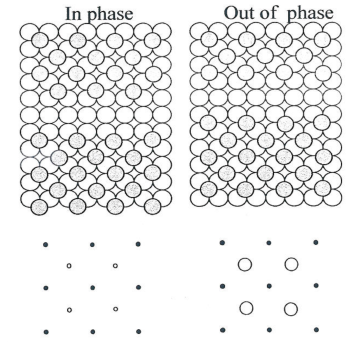
\includegraphics[scale=4]{figures/09_14.png}
	\caption{The real space model for two $2\times 2$ domains in phase and out of phase on a Ni(100) surface. Please note that in the out of phase mode the half order spots broaden if the domains are small enough.}
	\label{fig:22nileed}
	\end{center}
\end{figure}

\section{Dynamical Scattering and IV-Curves}
Strong oscillations appears in the intensity versus the  primary energy of the electrons due to the multiple scattering in the different layers. The resulting curves are called IV-curves as shown in \autoref{fig:ivni}.  The modulation are due to Bragg reflections into the crystal, but as the intensity into the bulk is exponentially damped and thus only  few layers contribute to this effect the modulation will be rather broad and the intensity will never go to zero completely.  By performing very detailed analysis of the electrons scattered in the surface and calculate the resulting beam intensity for a number of different beams as a function of energy it is possible to compare to the experimental measured IV curves.

\begin{figure}[h!]
	\begin{center}
	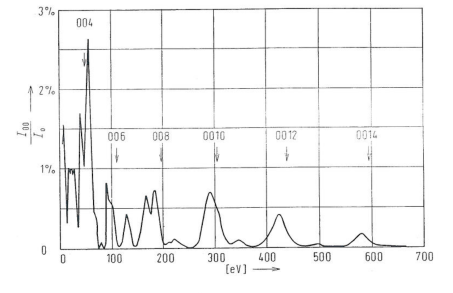
\includegraphics[scale=4]{figures/09_15.png}
	\caption{The $IV$-curve for Ni(100) at normal incidence.}
	\label{fig:ivni}
	\end{center}
\end{figure}

In this manner it is possible to obtain models which gives the best fit to the  data and obtain not only information on the two-dimensional structure in the surface but also the in depth distances between the different layers. In this manner it is for example possible to show that a clean  surface introduces an inward relaxation of the first layer towards the second while the second layer usually expands compared to the bulk lattice distances. The relaxations are typically \SIrange{-5}{10}{\percent} for the first layer and \SIrange{1}{3}{\percent} for the second layer. These relaxations are easily explained in terms of EMT. The outermost atoms are less coordinated and are therefore missing electron density. They can compensate for this and obtain the optimum electron density by shifting slightly towards the atoms below leading to the contraction. This on the other hand leads to a too high electron density for the atoms in the second layer which then expands to compensate, resulting in the so called Friedel oscillations which are exponentially damped into the material. Similarly detailed models can be constructed for adsorbate system and the distances can be extracted being the source of many accurate determinations of surface structures, see \cite{Somorjai}. Unfortunately this scheme only works for relative simple structures since the number of fitting parameter describing the IV-curves  are becoming too large for big unit cells like for instance a $\sqrt{19}\times\sqrt{19}$.

\section{Problems}
\begin{enumerate}
\item An often encountered reconstruction on metals are the missing row reconstruction of the fcc(110) surface (for example Pt(110)), where every second row of the surface are missing. Make a model of the surface in real space and its respective LEED pattern superimposed on the LEED pattern of the non-reconstructed surface. Discuss how and why this surface reconstruction appears.

\item Sulfur is adsorbed on a Ni(100) surface in a four-fold-hollow site. Draw the LEED pictures of a p($2\times 2$) and a ($2\times 1$) structure with two domains. How can you distinguish the two surfaces?

\begin{figure}[h!]
	\begin{center}
	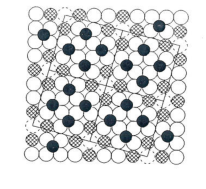
\includegraphics[scale=4]{figures/09_16.png}
	\caption{Hard sphere model of sulfur on Cu(100). Black and hatched spheres are sulfur atoms in first and second layer, respectively. Open circles and dotted circles are Cu atoms in first and second layer, respectively.}
	\label{fig:hardsphere_S_on_Cu}
	\end{center}
\end{figure}

\item Enclosed in figure \autoref{fig:hardsphere_S_on_Cu} is the hard sphere model for sulfur adsorbed on Cu(100) depicted. What is the Woods notation of the structure? What is the notation in the matrix notation? What is the coverage of sulfur and how manyu domains can be present? Draw the LEED pattern.

\item Make a few examples yourself in real space. Try for example $\sqrt3\times \sqrt3$ on a Fe(111) surface and find the resulting LEED pattern. Discuss whether the adsorbate coverage or position can be deduced for a LEED pattern.

\begin{figure}[h!]
	\begin{center}
	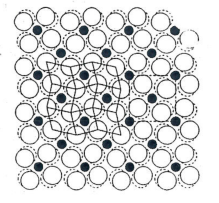
\includegraphics[scale=4]{figures/09_17.png}
	\caption{Hard sphere model of the C-NI($2\times 2$)p4g reconstruction. The black spheres are the carbon atoms while the open circles illustrates the Ni atoms displaced slightly from the original Ni(100) positions (dotted circles)}
	\label{fig:hardsphere_C_Ni}
	\end{center}
\end{figure}

\item In figure~\autoref{fig:hardsphere_C_Ni} is a hard sphere model for the clock reconstruction of carbon on Ni(100) depicted. The structure belongs to the symmetry group p4g and the resulting LEED pattern is the same as depicted in figure~\autoref{fig:culeed}. Notice that every second spot along the x and y axis is missing. Explain the reason for this peculiar behaviour.

\item In a LEED experiment we take a picture and observe a square pattern where the distance from (0,0) spit to the (1,0) spot is measured to be 4.1\,cm. Assume that the pictures is a one to one representation of the experiment. The radius of the LEED optics is 8.0\,cm and the primary energy is 72\,eV. What is the lattice distance of this crystal? If we assume there is an uncertaincy of 0.1\,cm on the measurement of the distance, what is then the resulting uncertaincy on the lattice distance determined? Discuss the energy of the electrons when being scattered at the surface.

\end{enumerate}


%\newpage
\chapter{Microscopy}
When investigating materials  and specifically catalysts it always of interest to get an impression for the three dimensional structure of the sample. This may be obtained through a strongly magnified picture of the material. Usually the conventional light microscopes are not supplying much help if we are going for the finer details such as nano-particles since  their resolution is limited by the wave length of the visible light to around 1$\mu$m. Thus if we are going for example nanometer or even atomic resolution we must turn to electron microscopes and scanning tunneling microscopes (STM). We have already in connection with scanning Auger seen that a scanning electron beam can make an excellent picture of the  three dimensional structure and that can be improved considerably by using several different methods for detection and by applying much higher energies (200-300 kV) of the electrons as it is done in dedicated electron microscopes. The ultimate resolution of electron microscopes allows a point resolution of about 1 �, sufficient for atomic resolution. The resolution is  strongly dependent on  the nature of the sample and it is in general not surface sensitive. The main emphasis here will, however, be put on the relative new  STM method. Compared to EM it is much less generally applicable, but on the other hand does  it offers a much more detailed view of the surface structure and dynamics, which have not been with in reach before. In STM is the  resolution  extremely good, less than 0.1 �, but it requires in general very flat  and well defined surfaces and is therefore in reality only applicable for model systems.

\section{The Scanning Probe Methods}

The idea of scanning probe microscopes is quite simple and comes now in several versions of which the most prominent are  the Scanning Tunneling Microscopy (STM)  and  Atomic Force Microscopes (AFM). The STM method was developed first by Binning and Roher   \cite{Roher1, Roher2, Roher3} (who got the Nobel prize for their invention) and this is also the most mature of the scanning probe methods see also \cite{STM}. Here a sharp tip (curvature of the order 100 �) is brought close to a surface and a low potential difference (the bias voltage) is put between sample and tip. Classically there should not be a current between the sample and tip, but as the distance gets small (5-10 �)  quantum mechanics takes over and the electron can now tunnel though the barrier. This leads to a current which can be measured and is typically set to be around 1 nA.  The experimental setup is shown schematically in Figure 10.1

\vspace*{11cm}

\noindent {\bf Figure 10.1} Schematic drawing of the STM setup.

\vspace{1cm}


The experiment can be performed in several modes i.e. constant current, or constant distance while scanning the tip over a desired surface area. The constant current mode is the most common. Here is the current kept constant by varying the tip-surface distance in a feed back loop. The tip is mounted on a piezo electric tube which can expand or contract dependent on the potential difference. Similarly is the scanning in the xy direction obtained by applying potential differences on a tube that is split in four parts. The coarse approach of the tip to the surface is taken care of by applying a so called inch worm also based on piezo electric elements. The scanning in the xy direction goes from � regime to a few  $\mu$m. The inch worm allows the tip to be move several mm per minute while the much more accurate z motion while scanning is taken care of by a tube that can expand or extract typically 1000 � with a typical resolution of 0.01� !!!. The hole arrangement is kept small to obtain high resonance frequencies and  mounted on a vibrational damped setup so external disturbances can be eliminated.  For obtaining a typical STM picture the tip is scanned 256 lines measuring in 256 point for each line. The scan rate is very fast and it takes between 1 and 10 seconds to obtain a picture. By acquiring subsequent picture it is possible to make movies of dynamical processes on the surface such as diffusion and chemical reactions. Usually a Tungsten tip is used. There are good recipes for preparing sharp tips which is necessary if the surfaces are not flat, but blunt tips prepared just by cutting a tungsten wire by a plier may also work since as long as just one atom is sticking further out than the rest this will conduct all the current as we shall see later.  The disadvantage of STM is  that it unfortunately only works on reasonable well defined flat conducting surfaces.

The other scanning probe microscopy method that should be mentioned in this context is AFM. The setup is in many ways similar to STM, although here the tip is mounted on a cantilever which is just a spring. When the tip is brought close to the surface will there be  van der Waals interaction due to coulomb interaction of quantum fluctuations in the tip and substrate. This interaction sets up a potential and the tip will first feel a force when it approaches the surface. This force can be measured by measuring how much the cantilever (spring) is bent knowing the force constant.  The forces involved are extremely weak (nano Newton) and very sensitive methods must be used to measure how much the cantilever is bent. This is typically done by shining laser light on the cantilever which is reflected into a position sensitive detector so the motion up and down can be measured. The hole arrangement is again mounted on a piezo electric scanner so it can be scanned over a desired area. In this manner it is possible to get atomic resolution on flat samples, or determining the  surface morphology on a larger scale. The advantage of this method is that it does not require a substrate that is conducting meaning that it can be used on real catalyst samples where the support material often is an oxide. The drawback is  that the shape of the tip, as for STM,  put rather strong restriction on the resolution  and the topography that can be depicted. Like STM  does the method not give any clue to the composition of the surface so this information must be obtained by using complementary methods like XPS. The AFM method still undergoes strong development and may be improved considerably  in the future.

In the following we shall concentrate on the STM since this is the superior method and where the most interesting research is performed at the moment.


\subsection{Theory of STM}

A relative simple and adequate theory for the tunneling effect seen in the STM was presented by Tersoff and Haman \cite{Tersoff}. Here we shall only give a brief review of the involved theory and derive an expression for the essential tunneling current. The experiment is shown schematically in Figure 10.2 where the energy levels of the electron in the tip and the sample are illustrated. Both are assumed to be free electron metals with monotonically density of states (DOS) around the Fermi level and work function $\phi_{\mu}$  for the tip and  $\phi_{\nu}$ for the crystal.  Figure 10.2 a illustrates the situation when the distance  between tip and surface is large. 

\vspace*{11cm}

\noindent {\bf Figure 10.2} Schematic drawing of the surface potential of the crystal and the tip.

\vspace{1cm}




The  distance in Figure 10.2b is now reduced to d and the tip is biased negatively with a few mV with respect to the crystal.
The potential for the electrons is reduced to a potential barrier with an average hight of $\phi = \frac{\phi_{\mu}   + \phi_{\nu}}{2}$ and as the wave functions for the electrons does not decay completely to zero they  may tunnel through the barrier. The expression for the tunnel current is in 1. order perturbation theory given by:
\begin{equation}
I=\frac{2\pi \mid e\mid }{\hbar}\sum_{\mu \nu}(f(E_\mu)(1-F(E_\mu)))\mid M_{\mu \nu} \mid  \delta (E_\mu + \mid e \mid V - E_\nu)
\end{equation}
where E$_{\mu}$ and E$_{\nu}$ are the energy relative to E$_F$ the Fermi level and
\begin{equation}
f(E) = \frac{1}{e^{\frac{(E-E_F)}{K_{B}T}} + 1}
\end{equation}
 is the Fermi function giving the occupation as a function of E. V is the applied voltage difference and if 
V$\mid e \mid \simeq $ 0 and T $\rightarrow$ 0 then f(E$_\mu$) $\simeq$ 1  for E$_\mu  < $ 0 and    f(E$_\nu$) $\simeq$ 0  for E$_\nu > 0$, thus electrons are tunneling from filled states in the  tip into the empty conduction states above the Fermi level of the  crystal. The delta function ensures energy conversation, i.e. it is assumed that the electrons do not undergo energy losses during the mechanism. This assumption is easily seen to be fulfilled  by  considering that typical bias voltages  are 10 mV and the universal curve discussed earlier. This will be truly ballistic electrons moving far into the crystal before undergoing energy losses. Using  V $\simeq$ 0 and the other  approximations we get 
\begin{equation}
I=\frac{2\pi  e^2 V }{\hbar}\sum_{\mu \nu}\mid M_{\mu \nu} \mid  \delta (E_\mu - E_F) \delta (E_\nu - E_F)
\end{equation}
The essential problem of calculating the tunneling matrix element $M_{\mu \nu}$ was solved by Bardeen \cite{Bardeen} giving
\begin{equation}
 M_{\mu \nu} = - \frac{\hbar^2}{2m} \int d\overrightarrow{S}(\Psi_ \nu^{\dag}\nabla\Psi_\mu-\Psi_\mu \nabla\Psi_\nu^{\dag}
\end{equation}
 Remembering  that i$\hbar \nabla$ is the moment operator it is seen that  this integral evaluates the flux of electrons though the  a surface S lying in the vacuum region.

In order to get any further we must introduce the appropriate wave functions. The wave functions at the surface of the crystal are straight forward  described by the two-dimensional Bloch expansion as:
\begin{equation}
\Psi_ \nu (\overrightarrow{r_\parallel},z) = \frac{1}{\sqrt{\Omega}} \sum _{G} a_G e^{i\overrightarrow{\kappa_G}\overrightarrow{r_\parallel}}e^{-z \sqrt{\kappa^2+\kappa_{G}^{2}}}
\end{equation}
where G is a surface reciprocal lattice vector,  $\Omega$ is a normalization volume, and  $\kappa$ is the decay constant of the surface wave into the vacuum region . $\kappa$ is given by
\begin{equation}
\kappa = \sqrt{\frac{2m\phi}{\hbar^2}}
\end{equation}
Thus the surface wave function is just an expansion on plane Bloch waves that are exponentially damped out in the vacuum region with the potential $\Phi$ as indicated in Figure 10.2. The evaluation of the tip wave functions $\Psi_\mu$ is much more difficult since its structure is not known in detail. One way to approach this problem is to assume that the end of the tip can be approximated by a sphere with radius R centered at position $\overrightarrow{r_0}$ as indicated in Figure 10.3. Then the tip waves can be approximated by s-waves of the type
\begin{equation}
\psi_\mu = \frac{1}{\sqrt{\Omega_t}}c_t \kappa R e^{\kappa R}\frac{e^{-\kappa \mid r-r_0 \mid}}{\kappa \mid r-r_0 \mid}
 \end{equation}
where now $\Omega_t$ is  the  normalization volume and c$_t$ is a normalization constant.

\vspace*{8cm}

\noindent {\bf Figure 10.3} Schematic drawing of the tunneling geometry.

\vspace{1cm}


The matrix element can now be calculated leading to 
\begin{equation}
M_{\nu\mu} = \frac{1}{\sqrt{\Omega_t}}\frac{4\pi \hbar^2}{2m}Re^{\kappa R}\Psi_\nu(\overrightarrow{r_0})
\end{equation}
inserting this in the equation for the current I we get
\begin{equation}
I = \frac{8\pi\hbar^3 e^2 R^2 V}{m}e^{\kappa R}D_t(E_F)\rho(\overrightarrow{r_0},E_f)
 \end{equation}
where D$_t  =  \frac{1}{\Omega_t}\sum_ {\mu} \delta(E_\mu-E)$ is the density of states per volume of the tip and
\begin{equation}
\rho(\overrightarrow{r},E_f) =\sum_{\nu} \mid\Psi_\mu \mid^2 \delta(E_\nu -E)
 \end{equation}
is the local density of states at the crystal . The surface wave functions are exponentially damped out in vacuum where the is a mean potential $\Phi$ resulting in
\begin{equation}
 \mid\Psi_\mu \mid^2  \propto e^{-2\kappa z}
 \end{equation}
leading to the final equation
\begin{equation}
 I   \propto e^{-2\kappa z} =e^{-1.025\sqrt{\Phi(eV)}z(�)}
 \end{equation}

The main result is that the current is exponentially dependent on the distance between the tip and the surface, mainly because the overlap between the empty and filled wave is dependent of the tails of the wave function out in the vacuum region. This explains why it is not extremely difficult to get a good and localized tip. Consider one atom on the tip that sticks out with just 1 � compared to the rest, then it will carry 90\% of the current. This also explains why it is possible to obtain atomic resolution in STM.
 Finally it should be mentioned that for  fixed tip conditions  we will probe the density of states (either empty if the tip is negatively biased or filled states if the tip is positively biased) of the crystal just below tip. Thus what is depicted in an STM experiment is {\bf not} the atoms but the density of states around the Fermi level. That this density varies around the atoms leading to the observed corrugation is not a surprise.

The above model involved many approximations and assumption, nevertheless, it captures the most important features of the STM experiment. Naturally there are regions where this picture will break down due to it simplicity. If for example the tip surface distance is getting very small the potential barrier will not be a simple average any longer and eventually there will be formed an contact. This contact can consist of a single atom and is then seen how the conductance becomes quantized. This is an interesting phenomena but beyond the scope of these notes. Also if the current is getting very high will this simple picture break down since we have completely neglected the interaction between the  tunneling electrons. Thus care must be exercised.



\subsection{Results from the Yellium Model}
In order to elucidate how adsorbates will be depicted in STM N. Lang \cite{Lang} undertook a number of investigations using  a simple model system. The tip was modeled by a Na atom adsorbed on a high electron density metal which can be described by the so called yellium model. Here the positive charge from the nucleies are smeared out and the free electron gas is solved on this positive background. One advantage of such models is that it is relative easy to map out the difference in eigenstate density introduced by adding an adsorbate to the yellium. Figure 10.4 shows such differences when Mo, Na, and S is adsorbed on a yellium. The calculation are only shown for m=0 component of the wavefunctions since it is these states that are mainly  responsible for  the tunneling current. The figure shows that Na introduces a resonance above the Fermi level while S introduces one below and all three components result in additional charge density at the Fermi level. 


Using this set up  and positioning the ``tip'' i.e. the yellium with an adsorbed  Na atom in front of another yellium it was shown that the current density was indeed localized to the Na atom as shown in Figure 10.5. The largest current density arrow is a factor of 25 bigger than the smallest current density j$_0$. The length and the thickness of the current arrows are proportional to 1+ln(j/j$_0$).
 
\vspace*{8cm}

\noindent {\bf Figure 10.4} Difference in eigenstate density between the yellium-adsorbate system and the clean yellium for different adsorbates as indicated, taken from \cite{Lang}

\vspace{1cm}  




\vspace*{8cm}

\noindent {\bf Figure 10.5}  Current density for a ``tip'' consisting of a Na atom adsorbed on a Yellium positioned in front of a clean yellium surface. The length and thickness of the arrows are proportional to 1+ln(j/j$_0$). Taken from \cite{Lang} 

\vspace{1cm}




If this ``tip'' is now used to scan over the another yellium where adsorbates like Na, S, and He have been adsorbed it is possible to estimate how much $\Delta$ s the tip have to be displaced vertically in order to keep the current constant when a small bias voltage is applied. This is depicted in Figure 10.6 showing that Na will appear as a much larger protrusion than S while He will be depicted as a depression in the yellium. This is in good agreement with Figure 10.4 showing that Na introduces a much higher electron density at the Fermi level than  S does and since the tunneling current was proportional to the density of states at the Fermi level it will lead to a larger retraction of the tip in the Na case. The He will naturally not adsorb at all, but will due to the Pauli principle exclude the electron leading to a lowing of density of states with respect to the clean surface. 

\vspace*{8cm}

\noindent {\bf Figure 10.6} Displacement of the ``tip'' in the  constant current mode for Na, S, and He adsorbed on yellium, taken from \cite{Lang}

\vspace{1cm}  


The important thing to be learned from this, is that adsorbates may not necessarily be depicted as protrusions, although they are geometrically. It all depends on the effective charge density at the Fermi level and it is well known that adsorbates like carbon, nitrogen, and  oxygen all are depicted as holes, since they are relative electronegative and removes charge density from the Fermi level. This also shows that we must know what sort of adsorbates we are dealing with. i.e. the experiment must be conducted under well defined conditions.

\section{Spectroscopy}
In all the considerations above the bias voltage was kept low so only the states around the Fermi level participated in the tunneling phenomenon. If we now relax this condition and used higher potentials V the tunneling current will be dependent on the density of states at higher energy levels, making it possible to map out DOS below and above the Fermi level doing spectroscopy. The  current can be approximated  by
\begin{equation}
I \propto \int_{E_F}^{E_F+\mid e \mid V} dE \rho_\nu(\overrightarrow{r_0,E}) \rho{}_\mu(E-\dim e \dim V)
\end{equation}
where $\rho_\mu$ is the total density of states of the tip and $\rho_\nu$ is the local density of the sample. The  $\rho_\nu$ can  be approximated by a product of the density at the surface times a penetration factor out into the forbidden vacuum region as:
\begin{equation}
 \rho_\nu(\overrightarrow{r_0,E}) \sim  \rho{}_\nu(E) e^{-\frac{2d\sqrt{2m(W-E+\frac{1}{2})\mid e \mid V}}{\hbar}}
\end{equation}
where W is the hight of the potential barrier.  This is intuitively easy to understand. The lower the energy E the broader and higher will the barrier be and the current will therefore be dampened exponentially. If we want to isolate $\rho{}_\nu(E) $ we must clean it from the influence of the penetration factor and $\rho_\mu$ . By measuring relations between I and V for a fixed distance and by plotting  (dI/dV)/(I/V) will any sharp feature in the surface (or tip) density of states become apparent. An example was given by Lang shown in Figure 10.7 where  the Na ``tip'' was used on a Ca atom adsorbed on yellium. The left panel shows the difference in density of states for the two adsorbates and the left panel shows the resulting (dI/dV)/(I/V) analysis. Only broad features are in general observed for metals so this method is, like UPS,  useless for elemental analysis.

\vspace*{9cm}

\noindent {\bf Figure 10.7} Left the introduced difference in density of states by adsorbing Na and Ca on yellium. Right the resulting (dI/dV)/(I/V) analysis, taken from \cite{Lang}

\vspace{1cm}  



It is though worth noticing that if we look at S adsorbed on the yellium we see that the appearance in a STM experiment will depend very much on the bias potential, since it, as shown in figure 10.8, leads to a reduced density of states at high voltages. Thus, as indicated in Figure 10.8 the S atom will appear as a protrusion for voltages below 1 volt, will vanish around 1.3 volt and become a depression for higher voltages. Thus the picture obtainable will be very dependent on the choosen bias voltage. This is in particular illustrated on semiconductors where there is a bandgap and dangling bond pairs to form occupied bonding states and empty anti bonding states at the surface. By making (dI/dV)/(I/V) analysis the various states can be found for a constant distance and by scanning  at well choosen voltages the different orbitals can be mapped out on the surface. 

\vspace*{11cm}

\noindent {\bf Figure 10.8} Left the introduced difference in density of states by adsorbing Na and S on yellium. Right the vertical displacement of the ``tip'' over the S atom as a function of bias voltage, taken from \cite{Lang}

\vspace{1cm}  

In the above we have assumed that the tip behaves metallic-like. Not much is in reality known for sure about the states of the tip and the ad atom actually conducting the current. Sometimes the tip changes in the middle of a scan and what earlier appeared as protrusions may suddenly in the middle of a frame be  depicted as depressions or visa versa. Such sudden and unexplained changes are often interpreted as tip changes, where the tip for example is picking up  an atom  from the surface changing its nature.


\section{Examples of STM Investigations}
STM has had a very strong impact on the field of surface science and STM have to some extent also revolutionized the structural investigation. Still it is not a trivial method to use like LEED where it is possible to obtain a LEED pattern within less than half an hour if the surface is well ordered.  It can be reasonably tricky to prepare the tip so that high resolution pictures can be  obtained. Sometimes, the STM  is working immediately, other times one may spend a day at the microscope and only occasionally see a structure. It is particularly difficult to obtain atomic resolution on metal surfaces since the corrugation here usually is less than 0.1 �.

The STM and LEED methods  complements each other in the sense that LEED rather fast gives an idea of the overall order on the surface, but not much information on the atomic level if that is not ordered. Here, on the other hand,  works the  STM very well. In principle  does STM  not require any order on the surface and domain boundaries and position of single atoms can be investigated in great detail. So in principle the STM is much more versatile, although it should be remembered, that just because we see an interesting structure within an area of 100 x 100 �$^2$, does it not need to be representative for the rest of the surface. Therefore several areas must  be investigated before any conclusions can be drawn. In the following shall we give a few  examples on the use of STM.

\subsection{Surface Structure}
Acquiring a STM picture of a surface structure actually provides us with a real space picture of the surface topography, although care should be exercised. Since  it is the electron density at the Fermi level we are mapping out atoms that sticks out from the surface may  not necessarily become depicted as protrusion. Usually it is possible to recognize the unit cell although that does not provide a solution to the structure. An example is shown in Figure 10.9 where the STM pictures and the LEED patter of the S-Cu(100) ($\sqrt{17} \times \sqrt{17}$)R14$^\circ$ is shown.

 Although it from  AES studies is known that this surface contain 8 sulphur atoms per unit cell only four of them can be identified as protrusions in the STM picture. The corresponding LEED pattern is quite complex as there are two domains. A model based on the STM picture have been proposed and is shown in Figure 10.10. 

\vspace*{9cm}

\noindent {\bf Figure 10.9} STM and LEED picture of the S-Cu(100) ($\sqrt{17} \times \sqrt{17}$)R14$^\circ$ structure, taken from \cite{Luigi}



\vspace*{9cm}

\noindent {\bf Figure 10.10} A schematic model of the S-Cu(100) ($\sqrt{17} \times \sqrt{17}$)R14$^\circ$ structure with 8 sulphur atoms per unit cell, taken from \cite{Luigi}

\vspace{1cm} 



 Sometimes it is possible to observe both regions of the clean metal and regions covered with an adsorbate so it is possible to extend the metal lattice into the adsorbate structure. This is demonstrated in Figure 10.11 taken from Besenbacher et al. \cite{Besenbacher1} where the STM picture of the Cu(110) and the missing row reconstructed O-Cu(110) (2x1) are shown. 

\vspace*{11cm}

\noindent {\bf Figure 10.11} 

\vspace{1cm} 


Also by detailed analysis of the surface as a function of adsorbate dosis is it possible to estimate how much of the substrate is being build into a new structure by following the mass transport of the substrate, i.e. following the  development of steps and holes made in the crystal as a function of dosis. By making movies of the oxidation of Cu(110) it  was  for example possible to suggest at structure for the high coverage structure O-Cu(110)c(6x2), which quite surprising, showed that Cu atoms were sitting highly uncoordinated on top of the previous formed missing row reconstructions as shown in figure 10.12 \cite{Besenbacher1}. A structure where the unit cell is very difficult to solve in the conventional LEED-IV analysis.

\vspace*{11cm}

\noindent {\bf Figure 10.12} 

\vspace{1cm} 

\subsection{ Two-Dimensional Alloys and Overlayers}
Since there is no help to be found from spectroscopic analysis for distinguishing two metals from each other it can be a difficult task to investigate metal overlayers and alloy formation. But again if  the development of the surface can be followed as a function of deposition time, changes can be related to the amount of metal added. It is in this manner possible to study growth and diffusion mechanisms even on homo epitaxial systems like Pt deposited on a Pt single crystal. Earlier, the  growth mechanisms on surfaces were classified into  three modes as  mentioned  in Chapter 6 (Frank-van der Merwe, Stranski-Krastanov, and Volmer-Weber growth modes). However, the STM have shown, that that was a much to simplified picture and that there is many other complex ways the growth process may proceed. Also alloy formation can be investigated and it was recently shown by use of STM that even metals which are known to be immiscible can form two-dimensional alloys in the surface. It has now been found to be a quite common phenomena \cite{Besenbacher2} and we shall here describe  one of the first systems that was found.

If Au is deposited on Ni(111) it was expected that the Au would grow epitaxial on the Ni surface because the system was known to be immiscible and the surface energy of Au is significantly smaller than Ni. The surprise was therefor big, when STM pictures, like the one shown in Figure 10.13, were measured \cite{Besenbacher3}. Since the coverage of the black hole increased with increasing Au dosis these were identified as being due to gold. At the same time also some very bright atoms appeared and it turned out to be Ni atoms pressed out from the surface by the gold. Thus a two-dimensional nearly random surface alloy was being formed in this case. Actually the Au atoms have been calculated to protrude by about  a quarter of an � from the Ni surface, but again due to the electron density around the Fermi level  they appears like depressions in the Ni lattice. This two-dimensional surface structure proved to be a very good way to control the  reactivity of Ni particles and a catalyst was later developed on that basis \cite{Science}.

\vspace*{11cm}

\noindent {\bf Figure 10.13} 

\vspace{1cm} 


An example of studying overlayers on the surface is the Co-Cu(111) system. Again the structures that was found when depositing Co at room temperature were not simple islands in the submonolayer regime. Instead,  two layer high islands were found surrounded by a single layer high island. By adsorbing CO it was possible to identify,  that the central island consisted of Co while the surrounding island consisted of Cu. An STM picture of CO on Co/Cu(111) at room temperature is shown in Figure 10.14 taken from \cite{Morten}. CO was only adsorbed on Co sites at this temperature, and the ($\sqrt{3}\times\sqrt{3}$)R30$^{\circ}$ of CO on Co can be recognized in the top layer \cite{Morten}. Around the apparent double layered Co island there is a Cu brim which with time will become double layered at room temperature. 

\vspace*{11cm}

\noindent {\bf Figure 10.14} 

\vspace{1cm} 



Based on such STM pictures with atomic resolution, a model was proposed which is schematically illustrated in Figure 10.15. Thus co-adsorption of for example CO made it possible to distinguish the Co from Cu. It should in this context be mentioned that it is usually very difficult to obtain pictures of CO adsorbed on surfaces, since these species diffuse very fast compared to the time scale of the STM experiment. Only in the saturation coverage regime will  the  CO structure  freeze out and pictures like the one shown in Figure 10.14 are  obtainable.


\vspace*{11cm}

\noindent {\bf Figure 10.15} 

\vspace{1cm} 


\subsection{Dynamics and Chemical Reactions}
By acquiring sequences of pictures it is possible to follow the dynamics on the surface if the processes are taking place on the same time scale as the measurements. This is mainly a matter of being able to control the temperature of the sample while scanning. Unfortunately, that is not a trivial problem, since the sample must be vibrationally isolated and any temperature difference may lead to thermal drift in the system. Nevertheless, there is a strong development in the field and there have recently been many studies both below and above room temperature. 

 For example can diffusion of ad atoms or adsorbates  be studied and by following their tow-dimensional movement  the diffusion constant can be extracted. Also regular chemical reaction may be followed. One example is the oxidation of methanol on the O-Cu(110) (2x1) structure where it has been shown that the reaction is very anisotropical and only takes place at the rim of the oxygen islands. This implies that at that particular temperature is the  mean field approximation not valid. Such experiment requires long time stability of the STM and surprisingly few good investigations have actually been performed. This is also an area of development, since there is a strong demand for being able to run the STM not only at elevated temperatures but also at elevated pressures, from the catalysis community. Any STM can run under ambient conditions, but the challenge is to get it running in atmospheres relevant to catalysis and study reactions at the surface. There have been attempts to obtain STM images of real catalysts, but sofar has it not been very successful. It is very difficult to  orient yourself on such non-ideal surfaces and find the active metal particles. Furthermore is there also the problem of the isolating support material. 





\section{Electron Microscopy}
Electron Microscopy is widely used giving us a visual impression of materials or biological samples in the regime where the light microscopes does not work any longer. Considering  the universal curve  it is obvious that these 100-400 keV electrons will penetrate way into the sample and the method is as such not a surface sensitive method, although it can be if combined with for example an Auger analyzer. There are many ways to detect the electrons used in the EM as shown in Figure 10.16 taken from \cite{Niemantsverdriet} and each of the methods adds complementary information on the sample  investigated.  

%\vspace*{11cm}

\noindent {\bf Figure 10.16} 

\vspace{1cm} 

The transmitted (TEM) or reflected (SEM) electrons may in the scanning mode be used for depicting the sample morphology. By measuring emitted x-rays (EDX), emitted electrons (Auger), or by measuring energy losses it is possible to make elemental identifications. The electrons may undergo diffraction, if there are favorable oriented crystalline particles so also crystallographic information may be obtained. An example  of a transmission electron micrograph, stimulating our imagination of a catalyst, is shown in Figure 10.17 where small  Rh particles are supported on a silica sphere  \cite{Datye}.


%\vspace*{11cm}

\noindent {\bf Figure 10.17} 

\vspace{1cm} 


 Another example is the highly undesired growth of carbon on Ni-catalyst as shown in Figure 10.18. Here it is seen how the carbon filaments grow out from the Ni-particles basically ruining the catalyst, taken from \cite{carbon}.

%\vspace*{11cm}

\noindent {\bf Figure 10.18} 

\vspace{1cm} 



EM microscopes usually comes in the conventional high vacuum regime (10$^-6$- 10$^{-7}$ mbar) or   in the UHV version (10$^{-10}$ mbar). But  recent development have made it possible to study samples under reasonable pressures (mbar regime) so catalysts can be studied under somewhat more realistic conditions following for example the dynamics as a function of gas composition. Care must naturally here be taken here since an 300 kV beam is not exactly innocent concerning introducing chemical reactions, that would not otherwise have been possible.





.
\newpage 
.
\newpage
%\newpage
\chapter{Ion Scattering Methods}

There are a wide number of other important methods in surface science and it is beyond the scope of these notes to treat them all. Nevertheless the ion scattering methods deserves to be mentioned briefly, since they are used widely and will be encountered quite often in the literature.

Previously we have seen how heavy ions like Ar could be used to remove atoms from the surface and how that combined with an analytical method like AES could be utilized to get information from deeper lying layers. In the following section we shall see how primarily light ions such as H$^+$ or He$^+$ can be used to actually identifying various elements at the (Ion Scattering Spectroscopy), and also how they in the high energy version can be used to make a non-destructive depth profile. Both methods come in more advanced version where also surface geometry can be investigated and serve as tool for structural investigations like LEED.


\section{Low Ion Scattering Spectroscopy}
The principle Low Energy Ions Scattering (LEIS) or just Ion Scattering Spectroscopy (ISS) is very simple and can be performed in many UHV champers in its basic version. All that is required is an ion gun and a bipolar analyzer so that the energy of positive ions instead of electrons can be measured in an angle resolved manner. Naturally the setup can be more advanced by having a well focused ion source so that lateral resolution can be obtained or with a movable analyzer so that the ions can be detected in various scattering geometries. In the following shall we only consider the simple version where the angle between the analyzer and the ion gun is fixed. The geometry is depicted in Figure 1. 

\vspace*{8cm}

\noindent {\bf Figure 11.1} Schematic drawing of the ISS setup.

\vspace{1cm}


\vspace*{8cm}

\noindent {\bf Figure 11.2} Calculated He$^+$ ion trajectories as a function of impact parameter. The energy of the He beam was 1 keV and the target atom is Yb.

\vspace{1cm}



ISS usually refers to primary energies of 1-2 keV energy of the ions. Preferentially He is used although heavier ions like Ne are also encountered. Very low ion doses are used in order not to create to much damage on the surface by sputtering processes. This is also one of the reasons for using lighter He ions. In this low  energy regime the ions interact nearly perfect through a binary collisions with the surface atoms. The method is vey surface senistive since it has a large scattering cross section $\sim ANGSTROM^{2}$ and thereby a large shadow cone see Figure 2 ensuring that most ions are not passing throug the first layer of the sample. Furthermore will most of the ions hitting the surface be neutralized ( > 99 \%) so very few are surviving the interaction as an ion.



 This make the method particularly surface sensitive since ions which penetrates into the surface or undergoes multiple scattering basically all will be neutralized and not detected in the electrostatic analyzer if they were to be scattered back. Since it is a simple binary collision there will be conservation of momentum and energy:
\begin{equation}
M_{i} \vec{v_{0}} = M_{i} \vec{v_{1}} + M_{s} \vec{v_{s}}
\end{equation}
and 
\begin{equation}
\frac{1}{2} M_{i} v_{0}^2 = \frac{1}{2}M_{i} v_{1}^{2}  + \frac{1}{2} M_{s} v_{s}^{2}
\end{equation}
where M$_i$, M$_s$, $\vec{v_0}$, $\vec{v_1}$, and $\vec{v_s}$ are the mass of the in coming ion, the mass of the surface atom, the velocity of the in coming ion, the velocity of the scattered ion and the velocity of the surface atom after the interaction.

After appropriate manipulation of the above equations the following ratio between the velocities of the in coming and out going ion can be found:
\begin{equation}
\frac{v_{1}}{v_{0}} = \frac{\pm \sqrt{M_{s}^{2}-M_{i}^2 sin^{2}(\theta)} + M_{i} cos(\theta)}{M_s+M_i}
\end{equation}

If the M$_{i}$ < M$_{s}$ the plus sign applies and the ration between the energy of the scattered ion is:

\begin{equation}
\frac{E_{1}}{E_{0}} =  \fracwithdelims[]{\sqrt{M_{s}^{2}-M_{i}^2 sin^{2}(\theta)} + M_{i} cos(\theta)}{M_s+M_i} ^{2}
\end{equation}

The equation shows that the energy of the ion after  the scattering event is only dependent on the initial energy of the ion, the angle $\theta$ and the mass of the surface atom. Since only the latter is unknown the mass of the surface atom can be determined. A typical ISS spectrum is shown in Figure 3. 

\vspace*{11cm}

\noindent {\bf Figure 11.3} Schematic drawing of the STM setup.

\vspace{1cm}


 The big advantage of ISS is that it basically restricted to probing the surface layer. Thus if  say  a 50-50 alloy is studied it is quite easily seen if one component segregates to the surface on cost of the other one. The same results are in principle obtainable from an AES or XPS study, but here will also deeper lying layers always contribute complicating the analysis. The mass resolutions is typically not very good (depends naturally on geometry and resolution power of the analyzer) and it is usually not possible to distinguish two neighbor elements such as nickel and copper unless special equipment and isotopically cleaned samples are used. In some specific cases the resolution between different element can be improved considerably by for instance using Ne$^{+}$ ions instead of He$^{+}$ ions, but great care should here be exercised that the surface is not damaged by sputtering during the measurements.

 In dedicated instruments it may be possible to make angle resolved measurements changing the  angle of the analyzer. By comparing such data to calculations of the absolute scattering cross section of the various atoms present on the surface and by making model calculation it is possible to extract information on the surface structure  just as could be done by modeling LEED IV-curves. Such  analysis is just as LEED restricted to well-behaved flat surfaces. Recently a dedicated instrument has been developed by  \cite{Brongersma} utilizing the advantages of the geometry of a CMA. By having the ion gun along the center of the analyzer, which is normal to the surface, and collecting scattered ions in a ring  of the cylinder, a huge gain in signal can be obtained. This means that it first of all is very fast to perform an analysis and secondly only very small doses of ions are necessary limiting the potential danger of destruction of the surface.

\section{High Energy Ion Scattering Spectroscopy}
This method will only be treated briefly here since it is not a general method as it requires access to high energy accelerators. An extensive  review of these methods can be found in \cite{feldman}. In a typical Rutherford Backscattering Spectroscopy (RBS) experiment  ions are used which has energies in the rage of 0.5-5 MeV. H$^{+}$, D$^{+}$and He$^{++}$ ions at these energies have a very small cross section for scattering and will therefore have a penetration depth of several $\mu$m into the material. By measuring the energy of the ions scattered back - $\theta$ = 170$^{\circ}$  - into a high energy ion detector it can in the same manner as for ISS be deduced which atoms the ion has encountered in the solid. The high energy  ion detector is typically a gold coated silicon wafer where the ions during de acceleration forms electron-hole pairs in the silicon in a number proportional to the energy of the incoming ion. Furthermore, as the ions will lose energy during penetration of the solid and since this energy loss can be estimated quite accurate is it possible to estimate the thickness the ions have penetrated in the sample. An example of a RBS is shown in Figure 4 where 3 MeV He$^{+}$ ions are back scattered ($\theta$ = 170$^{\circ}$) from a 4000 ANGSTROM thick Aluminum film with gold overlayers on both sides. Notice that the position of the front of the peaks reveals the element and the width the thickness of the various elements. Gold shows two peaks since ions scattered from the gold film on the back side will lose energy penetrating the aluminum film twice. Thus RBS analysis can be a powerful tool in many connections where it is necessary to analyze sandwich structure or diffusion profiles.



\vspace*{11cm}

\noindent {\bf Figure 11.4} Schematic drawing of the STM setup.

\vspace{1cm}



\section{Secondary Ion Mass Spectroscopy} Secondary Ion Mass Spectroscopy (SIMS)is a method very similar to ISS in the sense that also here are low energy ions used and the convectional UHV equipment will be sufficient. But instead of performing energy analysis of the back scattered ions  a mass analysis of particles sputtered away from the surface is performed as illustrated in Figure 5. This allows for a detection of which elements, fractions of molecules, or clusters have been present on the surface. The method is very sensitive and can in some cases measure down to ppm levels of impurities in a sample. This makes the method  particularly applicable in the microelectronic industry for characterizing for instance the silicon wafers for impurities and dopant.




\vspace*{11cm}

\noindent {\bf Figure 11.5} Schematic drawing of the SIMS setup.

\vspace{1cm}

Quantitative analysis is in general difficult in surface science, but it is a particular problem in SIMS due to the fact that the method relies only on the ions coming off the surface. Ideally all species should be detected if a correct composition should be extracted. As we saw for the ISS experiments the change of surviving as an ion was very little when interacting with the surface. Furthermore will this probability be very dependent on the element in question and the behavior of the surface. In an approximate picture a simple relation can be obtained \cite{Norskovlang} where the probability for obtaining positive ions is given by
\begin{equation}
P^{+} \propto e^{-\frac{(\Phi-A)}{\epsilon_{0}}} 
\end{equation}
where $\Phi$ is the work function of the surface, A is the affinity level of the atom leaving the surface, and $\epsilon_0$ is a variable dependent, among other things, on the hopping matrix element of the electron from the atom to the surface and the velocity normal to the surface of the atom leaving. Similarly is the probability for negative ions given by
\begin{equation}
P^{-} \propto e^{-\frac{(I-\Phi)}{\epsilon_{0}}} 
\end{equation}
where I is the ionization potential of the atom leaving the surface. It is now obvious why the probability for obtaining signal in SIMS will vary orders of magnitude for the different elements and why it is not possible to say anything about the surface composition from a spectra without taking due respect to the sensitivities of the different elements.  A SIMS spectrum of Si is shown in figure 6 together with an AES analysis of the same surface. The Sims analysis reveals may components which are not observed in the AES spectrum at all.That the probability also depends on the work function $\Phi$ makes things even worse since that will tend to vary strongly with the surface composition during a sputter profile. 


\vspace*{16cm}

\noindent {\bf Figure 11.6} Schematic drawing of the STM setup.

\vspace{1cm}

The quantitative analysis can naturally be considerably improved by using well known standards and the method is particular useful for measuring trace amounts of elements where methods like XPS and AES have  to give in due to their detection limit (roughly 1 atomic percent). SIMS can also be used for measuring bigger fragments sputter of the surface. For instance has SIMS is some special cases been used in catalysis to monitor whether certain intermediates may be present at the surface or not. Even bigger fragments can be analyzed, but then a conventional quadrupole mass spectrometer may not be sufficient any longer. Instead a Time of Flight technique (TOF)is used. This approach is particular useful when analyzing the fragments coming of polymer surfaces.


There are many interesting aspects to these ion based methods, but the reader is referred to Briggs and Seah for a thorough treatment \cite{briggs2} of this subject.




%\newpage
\part{The Gas Surface Interaction}


%\newpage
\chapter{Adsorption Processes}
\section{Introduction}

The gas-surface interaction and reactions on surfaces plays a very important role in many technologically important areas such as in corrosion, adhesion, synthesis of new materials, heterogeneous catalysis, etc. and  is therefore desirable to obtain a profound insigth in these processes. The impact of these studies have maybe been strongest in the field of heterogeneous catalysis where it has been possible to study quite realistic model systems since a large number of catalysts actually can be modelled by studies on well defined single crystals. Despite many years of effort do there, however, only exists very few examples, see fx \cite{Sciencepaper}, that surface science have let directly to the invention of a new catalyst. On the other hand has surface science provided the framework and necessary tools for understanding and designing new heterogeneous catalysts. The essential step in this process is first adsorption of the reactant on to the surface. Here they may react much easier with other reactants due to the changed chemical environnement on the surface. The proces should then be followed by a desorption process of the products cleaning of the surface making it available for new reactancts. In this part we shall focus on the physics and chemistry involved when gasses adsorbs on the surface and in particular metal surfaces. 

When an atom or molecule approaches the surface it will fell the potential energy surface set up by the metal atoms in the solid. The interaction is usually divided into two regime the physisorption regime and the chemisorption regime.

\section{Physisorption}

Physisorption is a weak interaction which is characterized by lack of a true chemical bond between the adsorbate and the surface, i.e. no electrons are shared. The physisorption interaction  is conveniently divided into to parts: A strongly repulsive part at close distances and a Van der Waals interactions at medium ranges.
\subsection{The van der Waals interaction}
When a  atom/molecule approaches a surface will the  electrons in the atom/molecule, due to quantum fluctuations,  set up  an dipole which induces an image dipole in the polarizable solid. Since this image dipole is of the oppersite sign and correlated with the fluctuation in the atom/molecule will the resulting force be attractive. In the following we shall construct a simple model which elucidates this phenomena. Consider a hydrogen atom with nuclus at origo located above the surface of a perfect conducting metal at the position $\vec{d}$= (0,0,d) and an electron at  $\vec{r}$ =(x,y,z). The image charges induced in the metal will be
\begin{equation}
q=\frac{1-\epsilon}{1+\epsilon}e = -e, \epsilon \rightarrow \infty
\end{equation}
The potential due to this image interaction is then given by 
\begin{equation}
V_{W}(\vec{d},\vec{r}) \propto -\frac{e^{2}}{2d} - \frac{e^{2}}{2(d+z)} + 2\frac{e^2}{\mid 2\vec{d}+\vec{r} \mid}
\end{equation} 
where the two first terms are due to the interaction between the nuclus and it image and the electron and its image of itself. The third term is due to the two repulsive cross terms. Simple Taylor expansion in powers of $\frac{\vec{r}}{\vec{d}}$ leads to 
\begin{equation}
V_{W}(\vec{d},\vec{r}) \propto -\frac{e^{2}}{d^3}(\frac{x^{2}}{2} + \frac{y^{2}}{2} + z^{2}) 
\end{equation}
Thus the net result is an attractive potential which goes as
\begin{equation}
V_{W}(d) \propto \frac{-C_{vW}}{d^3}
\end{equation}
where C$_{vW}$ is the so-called van der Waals constant for the system which is dependent on the polarizability of the atom and the responce of the metal. Notice that the interaction does not require a permanent dipole and rare gas atoms may therefore also physisorb on the surface. An effect that we later shall utilize to determine the overall areas of surfaces.
\subsection{The repulsive part}
The attraction naturally does not continue for small d since the  electrons of the atom/molecule now will begin to interact strongly with the electrons of the surface. The kinetic energy of the solid increase as they will have to orthorgonalize to the localized electrons of the atom as a consequence of the Pauli repulsion. Some energy will natually be  gained as the same electrons also become attracted to the positive nucleus, but this can by no mean compenate the repulsion that occurs when it is not possible to make a chemical bonding as is the case for the rare gases. A simple approximation of the potential in this regime is an exponential function 
\begin{equation}
V_{R}(d) \propto e^{-\frac{d}{\alpha}}
\end{equation}
 since the desity of the electrons is decaying in this manner away  form the surface.
The resulting potential 
\begin{equation}
V(d) = C_{R}e^{-\frac{d}{\alpha}}-\frac{-C_{vW}}{d^3}
\end{equation}
is shown in figure 2. The depth of the well is usually of the order a few kJ/mole or less and the minimum will be several � from the surface. Thus molecules that are physisorbed on the surface are not chemically altered, but conserves theirs spectrosopic characteristica of the gas-phase. 

The effect is very similat to the molecular van der Waals interaction which makes gasses condense in multilayers. Here the potential have a very similar form as it is of the same nature. Often a  Lennard-Jones (N,6)-potential is used which has the form 
\begin{equation}
V(d) = \frac{-C_{n}}{d^n}-\frac{C_{6}}{d^6}
\end{equation}
and in particular the n=6 is popular for matematical reasons, despite the fact that an exponential description as above usually give a better description of the repulsive part\cite{Atkins}. The attractive part goes in this case as d$^{-6}$ \cite{Atkins}.

\section{Chemisorption}
\subsection{The Hydrogen molecule}
Before we treat chemisorption on surfaces i may be helpfull to first consider the most simple chemical bonding we can think of namely the bonding in the hydrogen molecule. This is not all that simpel and we will therefore start out with a H$_{2}^{+}$ ion. Consider to hydrogen atoms far away from each other then the electronic wave functions can be described by $\Psi_{a}$ and $\Psi_{b}$ which are eigenfunctions to the atoms with the energy $\epsilon_{a}$ and $\epsilon_{b}$. I we start to bring these two atoms close we know they will form a chemical bonding and end up as a molecule. The procedure for modelling this is to construct a new weavefunction from the atomic orbitals and the method is referred to as the linear combination of atomic orbitals (LCAO) medthod. In the following we shall neglect the spin. Thus the new wave function for one electron will have the form
\begin{equation}
\Psi=c_{1}\Psi_{a} + c_{2}\Psi_{b}
\end{equation}
and the Hamilton will have the form 
\begin{equation}
H = (-\frac{\hbar^{2}}{2m_{e}})\nabla^{2} +  (\frac{e^{2}}{4\pi\epsilon_{0}}\biggl( -\frac{1}{r_{a}} - \frac{1}{r_{b}}  + \frac{1}{R}\biggl) 
\end{equation}
where r${a}$ and r$_{b}$ are the distance of the single electron to the nuclei a and b.
By using the variation principle and solving the secular equations
\begin{equation}
\Sigma_{i} C_{i}({\bf H_{ik}} - {\bf ES_{ik}}) = 0,
\end{equation}
where H$_{ik}$ are matrix elements of the hamiltonian and S$_{ik}$ are the overlap matrix elements. Note that the atomic wavefunction are not orthorgonal.  These equations have  solutions when the determinat vanishes i.e when
\begin{equation}
\begin{vmatrix} \alpha-E & \beta -SE \\ \beta - ES & \alpha - E\end{vmatrix}
\end{equation}
where  we have used 
\begin{description}
\item[S$_{aa}$]= 1 since $\Psi_{a}$ was already normalized.
\item[S$_{bb}$]= 1 since $\Psi_{b}$ was already normalized.
\item[S$_{ab}$]= S the overlap intergral
\item[$\alpha$]= H$_{aa}$ = H$_{bb}$ = $\int \Psi_{a}((-\frac{\hbar^{2}}{2m_{e}}\nabla^{2}) +\frac{e^{2}}{4\pi\epsilon_{0}}\biggl(-\frac{1}{r_{a}} - \frac{1}{r_{b}} + \frac{1}{R}\biggl))\Psi_{a}dV$
\item[$\beta$]= H$_{ab}$ = $\int \Psi_{b}((-\frac{\hbar^{2}}{2m_{e}}\nabla^{2}) +\frac{e^{2}}{4\pi\epsilon_{0}}\biggl( -\frac{1}{r_{b}} - \frac{1}{r_{a}} + \frac{1}{R}\biggl))\Psi_{b}dV$
\end{description}
The result is two energy levels of the form:
\begin{equation}
c_{a}=c_{b} , c_{a}=\frac{1}{\sqrt{2(1+s)}}, E_{+}= \frac{\alpha+\beta}{1+s}
\end{equation}
\begin{equation}
c_{a}=-c_{b} , c_{a}=\frac{1}{\sqrt{2(1-s)}}, E_{+}= \frac{\alpha-\beta}{1-s}
\end{equation}
The terms $\alpha$ and $\beta$ can be rewritten renembering that the eigenvalue of the atomic hamiltonias is just E$_{1s}$ i.e.
\begin{equation}
\alpha = E_{1s} +\frac{e^{2}}{4\pi \epsilon_{0} R}-j_{1}
\end{equation}
where
\begin{equation} 
j_{1} = \frac{e^{2}}{4\pi\epsilon_{0}} \int \Psi_{a}\frac{1}{r_{b}}\Psi_{a}dV
\end{equation}
is a positive quantity. In a semilar manner can $\beta$ be rewritten as 
\begin{equation}
\beta = (E_{1s} +\frac{e^{2}}{4\pi \epsilon_{0} R})S-k_{1}
\end{equation}
where 
\begin{equation} 
k_{1} = \frac{e^{2}}{4\pi\epsilon_{0}} \int \Psi_{a}\frac{1}{r_{a}}\Psi_{b}dV
\end{equation}
In this manner can the two solutions be written as 
\begin{eqnarray}
E_{+} = E_{1s} +\frac{e^{2}}{4\pi \epsilon_{0} R}-\frac{j_{1}+k_{1}}{1+S}\\
E_{-} = E_{1s} +\frac{e^{2}}{4\pi \epsilon_{0} R}-\frac{j_{1}-k_{1}}{1-S}
\end{eqnarray}
Since both j$_{1}$ and k$_{1}$ are positive  will we get a  an upward shidt of both levels and then a upeward and down ward splitting as shown in Figure 3. Notice that the downward shift thus is smaller than the upward shift. The energy gain by forming the H$_{2}^{+}$ ion is thus the energy gain by moving one electron from E$_{1s}$ down indo the E$_{+}$ state.

In reality we wanted to consider the hydrogen molecule. The gross effect just corresponds to filling to electrons into the diagram show in figure 3 although the splitting will chage quantitatively.  For a hydrogen molecule will we have the hamiltonian:  
\begin{equation}
H = (-\frac{\hbar^{2}}{2m_{e}})(\nabla_{1}^{2} +\nabla_{2}^{2}) +  \frac{e^{2}}{4\pi\epsilon_{0}}\biggl( -\frac{1}{r_{1a}} - \frac{1}{r_{1b}} - \frac{1}{r_{2a}} - \frac{1}{r_{2b}} + \frac{1}{r_{12}} + \frac{1}{R}\biggl) 
\end{equation}
and we will here  use the valence band approch instead of the LCAO method to construt the two electron wave functions i.e.
\begin{equation}
\Psi=c_{1}\Psi_{a}(\vec{r_{1}})\Psi_{b}(\vec{r_{2}})+c_{2}\Psi_{b}(\vec{r_{1}})\Psi_{a}(\vec{r_{2}})
\end{equation}
agan neclegting the spin. The procedure follows the schemme give above for the ion except that a few new terms arises due to the changes in the hamiltonian.
The result of these consideration gives the eigen values:
\begin{eqnarray}
E_{+} = 2E_{1s} +\frac{e^{2}}{4\pi \epsilon_{0} R} + \frac{j_{2}-2j_{1}+k_{2}-2k_{1}S}{1+S^{2}}\\
E_{-} = 2E_{1s} +\frac{e^{2}}{4\pi \epsilon_{0} R} + \frac{j_{2}-2j_{1}-k_{2}+2k_{1}S}{1-S^{2}}
\end{eqnarray}
where 
\begin{eqnarray}
j_{2}=\frac{e^{2}}{4\pi\epsilon_{0}} \int \Psi_{a}^2(\vec{r_{1}})\frac{1}{r_{12}}\Psi_{b}^2(\vec{r_{2}})dV_{1}dV_{2}\\
k_{2}= \frac{e^{2}}{4\pi\epsilon_{0}} \int \Psi_{a}(\vec{r_{1}})\Psi_{b}(\vec{r_{1}})\frac{1}{r_{12}}\Psi_{a}(\vec{r_{2}})\Psi_{b}(\vec{r_{2}})dV_{1}dV_{2}
\end{eqnarray}
Usually the term J=j$_{2}$-2j$_{1}$ and K=k$_{2}$-k$_{1}$S are introduced as the coulomb and exchange integral respectively  and both are negative. The dissociation energy (2E$_{1s}$-E$_{+}$) is found to be 303 kJ/mol which is somewhat lower that the experimental value of 432kJ/mol. This can be improved by using other trial functions and introduce configuration interaction. The bottom line is that the two atoms gains energy by forming a molecule sharing the electrons where both electrons are in the bonding state. The other state is refereed to a the anti bonding state. It is also easily seen why for example two he atoms may not form a He$_{2}$ molecule. Adding to more electrons to the in principle same diagram means that we are also filling the anti-bonding orbital. Since the anti-bonding state is shifted more up in energy than the bonding state is shifted down will it scost energy to establish such a bonding and the interaction will be repulsive.

The simple picture presented above for the LCAO-MO method can be extended to more complicated cases. In the case of diatomic molecules is it worth noting that the atomic orbitals must have the same symmetry with respect to to rotations about the internuclear axis if the should have non-zero overlap. Two adjacent orbitals like (1s,1s), (1s,2s) or any (xs,ys) will have non-zero overlap S. Similarly will (p$_{z}$,p$_{z}$), (1s,p$_{z}$) and (p$_{x}$,p$_{x}$) have non-zero overlaps whereas combinations like (1s,p$_{x}$) or (p$_{x}$,p$_{z}$) will have no overlap. Thus it is simple to see which atomic levels will interact and split up in bonding and anti-bonding orbitals. It can also easily be seen that only orbitals which has similar energy will interact. If we consider the interaction considered earlier we ended up with a secular determinat of the form
\begin{equation}
\begin{vmatrix} \alpha_{a}-E & \beta -SE \\ \beta - ES & \alpha_{b} - E\end{vmatrix}
\end{equation}
where we now are considering two different levels interacting. Solving for E leads to 
\begin{equation}
E = \frac{\alpha_{a}+\alpha_{b}-2S\beta \pm \sqrt{(\alpha_{a}-\alpha_{b})^{2} -4(\alpha_{a}+\alpha_{b})S\beta+4\beta^{2}-4\alpha_{a}\alpha_{b}s^{2}}}{2(1-s^{2})} 
\end{equation}
Considering the limit where the overlap is small S$\rightarrow 0$  and the difference between the two levels $\delta = \alpha_{b}-\alpha_{a}$ is larger than the interaction $\beta$
\begin{eqnarray}
E_{+}  \approx \alpha_{a}- \frac{\beta^{2}}{\delta}+S\mid \beta \mid 
E_{-}  \approx \alpha_{b}+ \frac{\beta^{2}}{\delta}+S\mid \beta \mid 
\end{eqnarray}
Thus the splitting decreases with the energy difference between the interacting levels. Notice that there always is a repulsion term due to the fact that the elctrons have to orthorgonalize. With these simple rules in mind we can now set up themolecular orbital energy diagrams for some simple diatomic molecules and some examples of N$_{2}$ and O$_{2}$ are given in Figure 4. The stability of the molecules can be estimated from the number of bonding orbitals filled compared to the number of anti-bonding orbitals. I.e. it is eaily seen that  N$_{2}$ molecule is much more stable than the O$_{2}$ molecule since in the latter the two additional electrons are located in anti-bonding orbitals.
Naturally the the accurate nature and energy of these bondings can and have been investigated in much greater detail, but the simple considerations presented here captures the essential aspects of the chemical bonding we need in order to proceed towards the phenomena chemisorption we set out to investigate. 

%\newpage
\chapter{Temperature Programmed Desorption and Reaction}
Temperature Programmed Desorption (TPD) and Temperature Programmed Reaction
(TPR) are  simple methods that relative fast can give an overview of:
\begin{itemize}
\item The bonding energy of simple adsorbates to a specific surface
\item On-set  temperatures of reaction or decomposition
\item Reaction pathways on the surface
\end{itemize}
all topics of great importance for studying catalysts since these are essential parameters which often are desired to manipulate in order to improve the overall performance. The  methods also sometime are referred to as Temperature Programmed Desorption Spectroscopy (TDS), Temperature Programmed Reaction Spectroscopy (TPRS), and a hole family of Temperature Programmed (Reduction, Oxidation, Sulfidation) Spectroscopies, but as the methods have nothing to do with spectroscopy we shall only apply the  acronyms TPD and TPR here.

\section{Experimental setup}
The simplest type of experiments with TPD or TPR are those made under UHV conditions on well defined single crystals. Here a single crystal can be mounted on  for example Tungsten wires and heated resistively. By having a feed back system is it possible to heat the crystal by a linear ramp as 
\begin{equation}
T = \beta t + T_0
\end{equation}
where $\beta$ is the heating rate and T$_0$ the start temperature. A typical heating rate is 1-5 Ks$^{-1}$. Non-linear ramps may also be used, but that makes the subsequent analysis very complicated.
Assume that we have already adsorbed some molecules on a surface and we positioned it in front of a mass spectrometer. We will then be able to measure what desorbs from the surface as a function of the crystal temperature. A typical setup is shown in Figure 11.1. The mass spectrometer (a quadrupole) is mounted inside a differential pumped shield so it does not measure  gasses released into the main chamber   where the crystal is mounted. The only connection between  the two chambers is hole with a diameter 3-4 mm. Doing TPD the crystal is brought up in  front of the hole ( $ < $ 0.5 mm) so only gas molecules desorbing from the central part of the crystal will be able do desorb into the mass spectrometer housing and be detected. In this manner, undesired signals from the surroundings, the sides of the crystal which are not well defined, and the wires, can be eliminated. It is naturally important that the differential pumping speed of the mass spectrometer is sufficiently high that it does not lead to substantial broadening of the TPD features. Although some broadening will always be  present since infinite pumping speed is usually not obtainable. (Infinite pumping speed is nearly obtained when studying desorption of for example metals, since they will stick to the first surface they encounter).

\vspace*{12cm}

\noindent {\bf Figure 11.1} Schematic drawing of an UHV setup for TPD and TPR. Taken from \cite{Yates}

\vspace{1cm}

As indicated in Figure 10.1 can this setup also be used for TPR by dosing the surface with molecules while performing a TPD. The crystal must then be retracted somewhat from the mass spectrometer housing so that  the beam of reactants can be dosed on the surface. In both cases the mass spectrometer can be multiplexed so many masses (typically 16) can be followed while heating. In many cases it can be very useful to use isotopically labeled atoms like C$^{13}$, N$^{15}$, and O$^{18}$ or Deuterium in order to determine different  reaction pathways on the surface.

Both experiments can also be performed on more complicated surfaces like real catalysts. One way is to mount a catalyst sample instead of the crystal. Again,  it is possible to obtain the same sort of information as with the single crystal. Unfortunately are the catalyst often rather inert to the reactants and relative high pressures (which may not be compatible  with UHV) are needed to obtain any reaction. The crystal or catalyst may naturally be exposed to high pressure if the UHV system is equipped with a high pressure cell, but it is very difficult to follow the reaction here. 

Thus another approach is to use a plug flow reactor containing a small amount of catalyst material, typical 0.1-1.0 g.  By heating the crystal in a flow of inert gas like He while ramping a TPD experiment can be performed. Similarly can also the TPR experiment be done if reactants are supplied at the same time. It should, however, in these sort of experiments be remembered that the catalyst usually is a very complex system, with a huge internal area and pore system. The processes we want to observe will therefore easily be transport limited, resulting in erroneous data for example due to   readsorption. The heating rate is therefore typically two orders of magnitude lower (Kmin$^{-1}$). The loss in intensity is more than compensated by the fact that 1 g of catalyst usually have areas that are 4-6 orders of magnitude higher than the single crystals used in the UHV experiments. The analysis of the TPD or TPR is made by analyzing the gas composition down stream. This can be done either by taking a small amount of gas into a  differentially pumped mass  spectrometer  or simply using a fast gas chromatograph. The mass spectrometer is prefered for small molecules and when good time resolution is essential. In this sort of experiment is it also possible to follow the reaction when the catalyst is either reduced or oxidized as mentioned above.  



\section{Theoretical background}
In the following we shall go though a model giving the essential rates of a  a desorption process. Since the desorption process may be considered as a special case of a reaction the same  picture  will also apply here.

In the TPD experiment we will typically have molecules like for example CO adsorbed on the surface. The molecules will  be bond to the surface in a potential with a well  depth E$_d$  shown schematically in Figure 11.2. At low temperatures the molecules will be in their vibrational ground state with energy $\frac{1}{2}\hbar \omega_0$. The mode where the entire molecule vibrates normal to  the surface. In the following we shall consider a group of such molecules distributed thermally  on the energy levels $\varepsilon$.
At temperatures kT $\gg \ \hbar \omega(\varepsilon)$ the number of trapped particles are given by 
\begin{equation}
n_{0}(T) = \int _{-E_d}^{0} g(\varepsilon)f_0(\varepsilon)d\varepsilon
\end{equation}
where $g(\varepsilon)$ is the density of the oscillator states in the potential and  
\begin{equation}
f_0(\varepsilon) = Z_{ads}e^{-\frac{(\varepsilon-\mu)}{kT}}
\end{equation}
is the occupation factor where Z is the partition function describing the internal degrees of freedom  and $\mu$ is the chemical potential.

\vspace*{11cm}

\noindent {\bf Figure 11.2} Schematic model of the potential for CO adsorbed on a surface.

\vspace{1cm}




We shall also  assume that the potential is sufficiently deep that E$_d$ $\gg$ T so that the population is dominated by energies at the bottom of the potential around kT. Thus we will approximate the density by  $g(\varepsilon) = \frac{1}{\hbar \omega(\varepsilon)} =  \frac{1}{\hbar \omega_0}$.
This approximation leads to
\begin{equation}
n_0(T) = \frac{kT}{\hbar \omega_0} Z_{ads} e^{\frac{\mu + E_d}{kT}} 
\end{equation}
In the TPD experiment there will in principle be no gas molecules present.  Thus the adsorbed molecules will be in thermal equilibrium with the surface except those which are at the top of the potential in the transition state. The flux of molecules leaving per time unit  here will be
\begin{equation}
J_0 = n_0 R 
\end{equation}
where R defines the desorption rate. The flux J$_0$ can be calculated from kinetic theory as an integral in phase space (x,p) of molecules in the transition state
\begin{equation}
J_0 = \int_{0}^{\infty}\frac{f(\varepsilon)}{h}dxdp 
\end{equation}
Using that $\varepsilon = \frac{p^2}{2m}$ is now the kinetic energy of the molecule and dx =  $\frac{pdt}{m}$ is the length traveled in time dt we get
\begin{equation}
J_0 dt = \frac{kT}{h}Z_{trans}e^{\frac{\mu}{kT}}dt 
\end{equation}
where Z$_{trans}$ is the partition function of the molecule in the transition state. By comparison of J$_0$ we get 
\begin{equation}
R = \frac{\omega_0 Z_{trans}}{2 \pi Z_{ads}} e^{\frac{-E_{d}}{kT}} 
\end{equation} There have been made several approximations here, but this equation  essentially describes the TPD experiment where the E$_d$ is the activation energy for desorption and $\frac{\omega_0 Z_{trans}}{2 \pi Z_{ads}}$ is the prefactor usually called $\nu$ leading us to the well know form
\begin{equation}
R = \nu e^{\frac{-E_{d}}{kT}}
\end{equation}
for a simple first order desorption mechanism like associatively bonded  CO  desorbing from a surface. The prefactor $\nu$ is often approximated by the attempt frequency $\frac{\omega_0}{2\pi}$ which is of the order 10$^{13}$ neglecting differences in the  partition function for the ground and the transition state.


The number of molecules desorbing from a surface per time unit $\frac{dN}{dt}$ (the quantity measured in the TPD experiment) will then be the number of molecules left on the surface  at time t times the desorption rate,  leading to the common differential equation
\begin{equation}
\frac{dN}{dt} =-N(t)\nu e^{\frac{-E_{d}}{kT}}
\end{equation}
using that $\theta = \frac{N}{N_0}$ where $N_0$ is the saturation coverage we get for a 1 order process
\begin{equation}
\frac{d\theta}{dt} =-\theta \nu e^{\frac{-E_{d}}{kT}}
\end{equation} This equation can be generalized to higher orders i.e. where two atoms like for example C and O recombines to form CO in order to desorb and the expression takes the form
\begin{equation}

\frac{d\theta}{dt} = \dot{\theta} = -{\nu}_n {\theta}^n e^{-\frac{E_d}{RT}}

\end{equation}

where ${\nu}_n$ is a modified pre-exponential factor, n is the order of the process,

E$_d$ the desorption energy [J/mole] and T the temperature of the surface.

These differential equations cannot be solved analytically and numerical solutions must be used to analyze the TPD curves. However, often a must faster approach can be used if we just want a rough estimate of E$_{d}$.

By differentiating the expression in equation  

with respect to the temperature, 

and putting this equal to 0 we find the temperature at which the TPD curve has it maximum T$_p$  

\begin{equation}

\frac{E_d}{R{T_p}^2} = {\nu}_n  n  {\theta}^{(n-1)}  \frac{1}{\beta}  e^{\frac{-E_d}{RT_p}}

\end{equation}

T$_p$ is identified from the measured spectrum.\\

The order of the process, n, is one 

if the desorption only requires one site as for CO on Ni(111) where CO adsorbs and desorbs as a molecule. 

If 2 atoms recombine to form the molecule we monitor, for example D$_2$ on 

Ni(111) the order is two.

For a n=1 process we have that

\begin{equation}

\label{eq:n=1a}

\frac{E_d}{R{T_p}^2} = {\nu}_1 \frac{1}{\beta}  e^{\frac{-E_d}{RT_p}}

\end{equation}

This can be rewritten as an expression which can be solved  iteratively

to determine E$_d$ from information about T$_p$, $\beta$ and an appropriate

initial guess of $\nu$, usually 10$^{13}$. This is a so-called Redhead analysis.

\begin{equation}

E_d = -RT_p ln(\frac{\beta E_d}{\nu_1 RT_p^2})

\end{equation}

where it should be noted that is assumed that $\nu$ and  E$_d$ are  independent of the coverage.
A similar analysis can be made for 2. order desorption.

From the above analysis it is seen how the TPD experiment can be used to estimated the bonding energy of adsorbed molecules to the surface. It should be noted that it actually the barrier for desorption we are probing see Figure 11.2 so in cases of activated processes this will be higher than the binding energy by the height of the activation energy for adsorption E$_a$.

In general will the both  $\nu$ and  E$_d$ depend on the coverage since the adsorbates will interact. This may lead to rather broad features and sometimes to more than one peak in the TPD curves, dependent on the nature of the lateral interaction. In figure 11.3 are a number of examples  for 0., 1., and 2. order desorption features shown with increasing repulsive interaction energies i.e. E$_d$=E$_0$-E$_{veks}\theta$. Please notice that attractive interaction may also occur leading to upward shifts in the TPD curves.



\vspace*{11cm}

\noindent {\bf Figure 11.3} Desorption curves for 0., 1., and 2. order desorption for different coverages and desorption energies  E$_d$=E$_0$-E$_{veks}\theta$.

\vspace{1cm}





\section{Examples}

In the following shall we give a few examples on TPD and TPR experiments.

In the first example shown in Figure 11.4 is the desorption of CO from a stepped Pd(112) crystal studied as a function of coverage \cite{Yates1}. This is a simple 1. order desorption process. Isotropical CO was used since that reduces the background in the TPD experiment (mass 30 usually is very low compared to mass 28 in most UHV chambers). Initially a feature at 500 K grows in with increasing dosages, but when that has saturated an other feature at around 400 K is getting filled. The TPD curve can be interpreted as being due to two different bonding sites on the surface, namely one at the steps (the high temperature feature) and one on the terrace (low temperature feature). From such an experiment using the above equations the difference in binding energy can easily be estimated. It should be noted that on the Pd(111) surface only the low temperature feature was observed.


\vspace*{11cm}

\noindent {\bf Figure 11.4} Desorption curves for CO from a Pd(112) single crystal as function of coverage.

\vspace{1cm}

The second example is desorption of hydrogen from Cu(100) shown in figure 11.5 \cite{Rasmussen}. In this particular experiment the Cu(100) surface was exposed to atomic hydrogen since the sticking of molecular hydrogen is very low. This process  is modeled reasonably well below 0.5 ML by a second order process as expected, but it is clearly seen that the model breaks down at the higher coverages. The exponential behavior of the desorption rate at the saturation coverage of 1ML is a typical finger print of a reconstruction of the surface. It is indeed known that this surface reconstruct forming a ``clock'' 2x2 reconstruction. The reconstruction is stabilized by the high coverage of atomic hydrogen, but when some of the hydrogen starts to desorb the rest will become less stable leading to the exponential desorption behavior in the high coverages regime.

The TPD can also be used to follow reactions on the surface. For example  when and how does formate decompose on a Cu(100) surface. This is illustrated in Figure 11.6 taken from \cite{HonCu}. The formate was either synthezied from a gas mixture of CO$_2$ and H$_2$ in a high pressure cell or made by dosing formic acid onto the surface in the UHV chamber. (In this manner it was actually possible to prove that the intermediate made in the high pressure cell was formate.) Formate is a very stable compound and it first decomposes at around 430 K into CO$_2$  and atomic hydrogen. 


\vspace*{8cm}

\noindent {\bf Figure 11.5} Desorption curves  H$_2$ from a Cu(100) single crystal as function of coverage. Notice the sharp feature at high coverage indicative of a reconstruction \cite{Rasmussen}.


\vspace*{9cm}

\noindent {\bf Figure 11.6}  TPD curves from formate. Upper panel:  Formate deposited by dosing formic acid.  Lower panel: Formate synthesized in a high pressure cell (2 bar) from a mixture of CO$_2$ and H$_2$. Taken from \cite{HonCu}





 As we saw in Figure 11.5 will hydrogen desorb already at around 300 K so the hydrogen released from the decomposing formate will immediately desorb. Similarly is CO$_2$ bound very weakly on Cu(100) so the desorption features observed are in reality probing the decomposition rate as the desorption rates of CO$_2$ and H$_2$  will be in equilibrium all the time.

Figure 11.7 shows an example of an TPR experiment performed under UHV conditions. Here deuterated methanol is dosed to a Ni(111) surface at different rates and the amount of methanol, CO, and deuterium is measured simultaneously. It can in this manner be seen that no reaction takes place  at the low temperature where the crystal is just becoming saturated by associatively adsorbed methanol. The surface is in this temperature regime just  reflecting the methanol beam  into the mass spectrometer resulting in a constant signal. 


\vspace*{11cm}

\noindent {\bf Figure 11.7} A TPR experiment under UHV conditions. Deuterated methanol is dosed while the crystal temperature is ramped. The desorbed species like methanol, CO, and D$_{2}$ are followed by the mass spectrometer. Taken from \cite{Yates2}.

\vspace{1cm}




 When reaching 250 K some methanol desorbs associatively ($\alpha$ peak) and some deprotonates forming methoxy species. At around 300 K the methoxy species starts to decompose spilling deuterium out on the surface, which  leads to protonation of some of the methoxy species ($\beta$ feature) and deuterium desorption. This leaves empty sites on the surface so that methanol is being consumed seen as a dip in the signal. By continuing heating the CO also will also start to desorb and the consumption persist since the surface is now basically clean. This demonstrates, that such a TPR experiment fairly rapidly can give a over view of the ongoing reactions. It could now be combined with a simultaneous oxygen dose and it can then be observed how the methanol may be oxidized into for example formaldehyde on a Cu sample.


TPD and TPR curves obtained from plug flow reactors are in principle very similar to the well defined examples shown above except for the problems mentioned concerning the transport phenomena. Naturally will  the TPD features in general be broader since there  always will be more than one specific site contributing to the desorption energy in a real catalyst.  Also great care must  be taken to obtain a uniform flow  in the reactor.  By taking care of these problem  it has in several cases been possible to obtain TPD curves which, when correcting for the different heating rates and crystal planes present, can be compared to  results obtained on single crystals.


Finally, a warning should be issued concerning TPD and TPR experiments in general. None of these experiment are in thermal equilibrium since we are ramping the temperature all the time. Therefor other processes make also take place at the same time obscuring some of the reactions taking place. An example is the adsorption on metal overlayers or alloys that are not stable. Consider for example the Co-Cu(111) system mentioned earlier. The CO adsorbed on the Co island will be destabilized by the Cu atoms segregating to the top of the Co islands while heating. This will  happen around the same temperature  as the desorption of the  CO molecules. Thus the  measured CO TPD will therefore not represent the true binding energy of CO on Co, but also the energy gained by segregating Cu to the surface. 
%\newpage
\chapter{Modelling Chemical Processes on Surfaces}

%include{chap15}
%\newpage
\chapter{Dynamics at Surfaces}
\section{Formation of Super Sonic Molecular Beams}
\section{Elastic and Reactive Scattering at Surfaces}
\section{Electron and Photon Induced processes at Surfaces}
%\include{chap17}



\begin{thebibliography}{99}
\addcontentsline{toc}{chapter}{Bibliography}

\bibitem{Zangwill} A. Zangwill, ``Physics at Surfaces'', Cambridge University Press, Cambridge (1988) ISBN 0-521-34752-1.

\bibitem{Somorjai} G. Somorjai,``Introduction to Surface Chemistry and Catalysis'',Wiley and Sons, New York (1994) ISBN 0-471-03192-5.

\bibitem{Hudson} J. B. Hudson ``Surface Science'', Wiley and Sons, New York (1998), ISBN 0-472-25239-5.

\bibitem{Niemantsverdriet} J. W. Niemantsverdriet, ``Spectroscopy in Catalysis'', VCH, Weinheim (1995), ISBN 3-527-28726-4.

\bibitem{Ertl} G. Ertl and J. Kuppers, ``Low energy electrons and Surface Chemistry'' VCH Weinheim (1985), ISBN 3-527-26056-0.

          \bibitem{briggs} D. Briggs and M. P. Seah, ``Practical
          Surface Analysis'', Wiley (1990) ISBN 0 471 92081 9.

             \bibitem{feldman}L. Feldman and J. W.
          Mayer,``Fundamentals of Surface and Thin Film Analysis'',
          North-Holland (1986) ISBN 0 444 00989 2.


             \bibitem{woodruff} D. P. Woodruff and T. A.
          Delchar,``Modern techniques of surface science'', Cambridge
          University Press (1986) ISBN 0 521 35719 5.

%Chapter 2 ***********************************************



          \bibitem{roth} A. Roth, ``Vacuum Technology'', North Holland
          (1990), ISBN 0 444 86027 4.

             \bibitem{Feynman} R. P. Feynman, R. B. Leighton, and M.
          Sands,``The Feynman Lectures'' Vol II. Addison-Wesley
          Publishing Company (1975).



             \bibitem{siegbahn1}  K.  Siegbahn,  C.  N.  Nordling,   K.
          Hamrin, J. Hedman, G. Johansson, T. Bergmark, S. E. Karlson,
          I. Lindgren, and B. Lindberg. ``ESCA, Atomic, Molecular, and
          Solid  State  Structure  Studied  by   Means   of   Electron
          Spectroscopy'', Almqvist and Wiksells, Uppsala, Sweeden, (1967).



             \bibitem{krause} Krause and Ferreria, (1975).

          \bibitem{chorkendorff}  I.  Chorkendorff,  J.  Onsgaard,   J.
          Schmidt-May, and R. Nyholm, Surf. Sci. 160 (1985) 587.


          \bibitem{gerken} F. Gerken, PhD Thesis,  HASYLAB,  Hamburg,
          Germany, (1982).

          \bibitem{shirley} D. A. Shirley, Topics in Applied  Physics,
          27, (19xx).



             \bibitem{wertheim} G. K. Wertheim and L.  R.  Walker,  J.
          Phys. F: Metal Phys, 6 (1976) 2297.



          \bibitem{doniach} S. Doniach and  M.  Sunjic,  J.  Phys.  C:
          Solid St. Phys, 3 (1970) 285.

          \bibitem{perkin} C. D. Wagner, W. M. Riggs, L. E. Davis,  J.
          F. Moulder,  and  G.  E.  Muilenberg,  ``Handbook  of  X-ray
          Photoelectron Spectroscopy'', Perkin-Elmer Corporation.

          \bibitem{ghosh} P. K. Ghosh, ``Introduction to Photoelectron
          and Auger Spectroscopy'', Wiley-Interscience Publishers, New
          York, (1983).

          \bibitem{shofield} J. H. Schofield, J. Electron Spectrosc. 8
          (1976) 129.


             \bibitem{chorkendorff2} I. Chorkendorff, I. Alstrup,  and
          S. Ullmann., Surf. Sci. 227 (1990) 291.

% Chapter 5 UPS*********************************************


\bibitem{Plummer} E. W. Plummer and W. Eberhart, Adv. Chem. Phys. 49 (1982) 533.
\bibitem{Andersen} J. N. Andersen I. Chorkendorff, J. Onsgaard, J. Ghiejsen, R. L. Johnson, and F. Grey, Phys. Rev. B 37 (1988) 4809.
\bibitem{Neddermeyer} P. Heimann, J. Hermanson, J. Miosga, and H. Neddermeyer Phys. Rev. B 20 (1979) 3059.
\bibitem{Kevan} S. D. Kevan, Phys. Rev. Lett. 50 (1983) 526.
\bibitem{Berglund} C. N. Berglund and W. E. Spicer, Phys. Rev. 136 A (1964) 1030 ibid. 1044.
\bibitem{Gustafson} T. Gustafson and E. W. Plummer, in Photoemission and Electronic Properties of Surfaces; Ed B. Feuerbacher, B. Fitton, and R. F. Willis,Wiley, Chicchester, p53 (1978).

%chapter 6 AES**********************************************


         \bibitem{wentzel} G. Wentzel, Z. Phys. 43 (1927) 524.

             \bibitem{handbook}  L.  E.  Davis,   N.   C.   Macdonald,
          P. W. Palmberg, G. E. Riach. and R. E. Weber, ``Handbook  of
          Auger Spectroscopy'', Perkin-Elmer Corporation.

             \bibitem{chorkendorff3} I.  Chorkendorff,  J.  N.  Russel
          Jr., and J. T. Yates Jr., J. Chem. Phys 86 (1987) 4692.

             \bibitem{briggs2} D. Briggs and M. P. Seah, ``Practical
          Surface Analysis'' Volume II, Wiley (1990) ISBN.




          \bibitem{sigmund}  P.  Sigmund,   ``Sputtering   by   Ion
          Bombardment;  Theoretical  Concepts''   in   Sputtering   by
          Particle Bombardment I, Editor R. Behrisch.  Springer-Verlag
          New York, (1982). Chapter 2.

          \bibitem{sigmund2} P. Sigmund, Phys. Rev. 184 (1969) 383.

          \bibitem{behrisch}             R. Behrisch.  Sputtering   by
          Particle Bombardment I and  II,  Springer-Verlag  New  York,
          (1982). Chapter 2.

          \bibitem{zalar} A. Zalar, Thin Solid Films 124, (1985) 223.

          \bibitem{hoffman} S. Hoffmann, Chapter 4 in D. Briggs and M.
          P.  Seah,  ``Practical  Surface  Analysis''Volumen  I,  Wiley
          (1990) ISBN 0 471 92081 9.

          \bibitem{alstrup} N. C. Alstrup, PhD Thesis, DTU (1993).
% Chapter 8 ****************************************************'
\bibitem{Ibach}  H. Ibach and D. L. Mills, ``Electron Energy Loss Spectroscopy and Surface Vibrations'' Academic Press, New York (1982).
\bibitem{Bruckmann} T. Bruckmann, S. Lehrwald, G. Kisters, and H. Ibach, (1990).
\bibitem{Formate} P. A. Taylor, P. Rasmussen, C. V. Ovesen, P. Stoltze, and I. Chorkendorff, Surf. Sci. 261 (1992) 191.
\bibitem{Bradshaw} A. M. Bradshaw, Surf. Sci. 11/12 (1982) 712.
\bibitem{Barnes} M. R. Barnes and R. F. Willies, Phys. Rev. Lett. 41 (1978) 1729.
\bibitem{Bailey}  S. Bailey, G. Forment, J. W. Snoeck, and K. C. Waugh, Catal. Lett. 30 (1995) 99.


% Chapter 9 LEED***********************************************

\bibitem{Kittel} C. Kittel, Elementary Solid State Physics: A Short Course, Wiley, New York, 1962.
\bibitem{Ashcroft} N. W. Ashcroft and N. D. Mernib, Solid State Physics, Holt-Saunders, Philadelphia, 1976.
\bibitem{Davidson}  C. J. Davidson and L. H. Germer, Phys. Rev. 30 (1927) 705.
\bibitem{Pendry} J. B. Pendry, Low Energy Electron Diffraction, Academic Press, New York 1974.
\bibitem{Hove} M. A. van Hove and  S. Y. Tong, Surface Crystallography by LEED, Springer, Berlin 1979.
\bibitem{Heinz} K. Heinz and K. Muller, in Structual Studies of Surfaces, Springer Tracts in Modern Physics, vol 91. Springer Berlin 1982.
\bibitem{HonCu} P. A. Taylor, P.B. Rasmussen, C. V. Ovesen, P. Stoltze, and I. Chorkendorff, Surf. Sci. 261 (1992) 191.
\bibitem{Shiff} L. I. Schiff, ``Quantum Mechanics'' McGraw-Hill Tokyo (1968).
\bibitem{Merzbacher} E. Merzbacher, ``Quantum Mechanics'' Wiley New York (1970).




% Chapter 10***********************************
\bibitem{Roher1} G. Binnig, H. Roeher, C. Gerber, and E. Weibel, Appl. Phys. Lett. 40 (1982) 178.
\bibitem{Roher2} G. Binnig, H. Roeher, C. Gerber, and E. Weibel, Phys. Rev. Lett. 49 (1982) 57.
\bibitem{Roher3} G. Binnig, H. Roeher, C. Gerber, and E. Weibel, Phys. Rev. Lett. 50 (1983) 120.
\bibitem{STM} Scanning Tunneling Microsopy I, II, III, Springer Series in Surface Science Ed: R. Wiesendanger and H. J. Guntherrodt,  (1993)  Berlin, ISBN 3-540-56317-2.
\bibitem{Tersoff} J. Tersoff and D. R. Hamann, Phys. Rev. Lett 50 (1983) 1998.
\bibitem{Bardeen} J. Bardeen, Phys. Rev. Lett. 6, (1961) 57.
\bibitem{Lang} N. Lang, Chapter 2 in Scanning Tunneling Microsopy  III, Springer Series in Surface Science, Ed: R. Wiesendanger and H. J. Guntherrodt,  (1993)  Berlin, ISBN 3-540-56317-2.
\bibitem{Luigi} M. L Colaianni and I. Chorkendorff, Phys. Rev. B 50 (1994) 8798.
\bibitem{Besenbacher1} F. Besenbacher, Rep. Prog. Phys. 59 (1996) 1737.
\bibitem{Besenbacher2} F. Besenbacher, Chapter 10 in``Techenical Physics of Solid Surfaces and Heterogeneous Catalysis", Ed. D. King and  D. P. Woodruff.
\bibitem{Besenbacher3} L. Pleth Nielsen, PhD Thesis from University of �rhus, Denmark (1996).
\bibitem{Science}  F. Besenbacher, I. Chorkendorff, B. S. Clausen, B. Hammer, A. M. Molenbroek, and J. K. N�rskov, Science 279 (1998) 1913.
\bibitem{Morten} M. �. Pedersen, I. A. Bonicke, E. L�gsgaard, I. Stensgaard, A. Ruban, J. K. N�rskov, and F. Besenbacher, Surf. Sci. 387 (1997) 86.
\bibitem{Datye} A. K. Datye and  N.J. Long, Ultramicroscopy 25 (1988) 203.
\bibitem{carbon} J. R. Rostrup-Nielsen, {\em Catalytic Steam Reforming} Catalysis- Science and Technology. Edited by J. R. Anderson and M. Boudart, Springer-Verlag, Berlin 1984, ISBN 3-540-12665-1.

%Chapter 11************************************
\bibitem{Yates} S. M. Gates, J. N. Russel Jr., and  J. T. Yates Jr., Surf. Sci. 159 (1985) 233.
\bibitem{Yates1} H. R. Siddiqui, X. Guo, I. Chorkendorff, and J. T. Yates Jr., Surf. Sci. 191 (1987) L813.
\bibitem{Rasmussen} P. B. Rasmussen and I. Chorkendorff, Surf. Sci. 248 (1991) 35.
\bibitem{Yates2} J. N. Russel Jr., I. Chorkendorff, and J. T. Yates Jr., Surf. Sci. 183 (1987) 316.


%Chapter 11************************************
\bibitem{Brongersma} ???
\bibitem{Norskovlang} N. D. Lang and J. K. N�rskov, Physica Scripta 6 (19983) 15.
\end{thebibliography}
\end{document}

